\documentclass[twoside]{book}

% Packages required by doxygen
\usepackage{fixltx2e}
\usepackage{calc}
\usepackage{doxygen}
\usepackage[export]{adjustbox} % also loads graphicx
\usepackage{graphicx}
\usepackage[utf8]{inputenc}
\usepackage{makeidx}
\usepackage{multicol}
\usepackage{multirow}
\PassOptionsToPackage{warn}{textcomp}
\usepackage{textcomp}
\usepackage[nointegrals]{wasysym}
\usepackage[table]{xcolor}

% Font selection
\usepackage[T1]{fontenc}
\usepackage[scaled=.90]{helvet}
\usepackage{courier}
\usepackage{amssymb}
\usepackage{sectsty}
\renewcommand{\familydefault}{\sfdefault}
\allsectionsfont{%
  \fontseries{bc}\selectfont%
  \color{darkgray}%
}
\renewcommand{\DoxyLabelFont}{%
  \fontseries{bc}\selectfont%
  \color{darkgray}%
}
\newcommand{\+}{\discretionary{\mbox{\scriptsize$\hookleftarrow$}}{}{}}

% Page & text layout
\usepackage{geometry}
\geometry{%
  a4paper,%
  top=2.5cm,%
  bottom=2.5cm,%
  left=2.5cm,%
  right=2.5cm%
}
\tolerance=750
\hfuzz=15pt
\hbadness=750
\setlength{\emergencystretch}{15pt}
\setlength{\parindent}{0cm}
\setlength{\parskip}{3ex plus 2ex minus 2ex}
\makeatletter
\renewcommand{\paragraph}{%
  \@startsection{paragraph}{4}{0ex}{-1.0ex}{1.0ex}{%
    \normalfont\normalsize\bfseries\SS@parafont%
  }%
}
\renewcommand{\subparagraph}{%
  \@startsection{subparagraph}{5}{0ex}{-1.0ex}{1.0ex}{%
    \normalfont\normalsize\bfseries\SS@subparafont%
  }%
}
\makeatother

% Headers & footers
\usepackage{fancyhdr}
\pagestyle{fancyplain}
\fancyhead[LE]{\fancyplain{}{\bfseries\thepage}}
\fancyhead[CE]{\fancyplain{}{}}
\fancyhead[RE]{\fancyplain{}{\bfseries\leftmark}}
\fancyhead[LO]{\fancyplain{}{\bfseries\rightmark}}
\fancyhead[CO]{\fancyplain{}{}}
\fancyhead[RO]{\fancyplain{}{\bfseries\thepage}}
\fancyfoot[LE]{\fancyplain{}{}}
\fancyfoot[CE]{\fancyplain{}{}}
\fancyfoot[RE]{\fancyplain{}{\bfseries\scriptsize Generated by Doxygen }}
\fancyfoot[LO]{\fancyplain{}{\bfseries\scriptsize Generated by Doxygen }}
\fancyfoot[CO]{\fancyplain{}{}}
\fancyfoot[RO]{\fancyplain{}{}}
\renewcommand{\footrulewidth}{0.4pt}
\renewcommand{\chaptermark}[1]{%
  \markboth{#1}{}%
}
\renewcommand{\sectionmark}[1]{%
  \markright{\thesection\ #1}%
}

% Indices & bibliography
\usepackage{natbib}
\usepackage[titles]{tocloft}
\setcounter{tocdepth}{3}
\setcounter{secnumdepth}{5}
\makeindex

% Hyperlinks (required, but should be loaded last)
\usepackage{ifpdf}
\ifpdf
  \usepackage[pdftex,pagebackref=true]{hyperref}
\else
  \usepackage[ps2pdf,pagebackref=true]{hyperref}
\fi
\hypersetup{%
  colorlinks=true,%
  linkcolor=blue,%
  citecolor=blue,%
  unicode%
}

% Custom commands
\newcommand{\clearemptydoublepage}{%
  \newpage{\pagestyle{empty}\cleardoublepage}%
}

\usepackage{caption}
\captionsetup{labelsep=space,justification=centering,font={bf},singlelinecheck=off,skip=4pt,position=top}

%===== C O N T E N T S =====

\begin{document}

% Titlepage & ToC
\hypersetup{pageanchor=false,
             bookmarksnumbered=true,
             pdfencoding=unicode
            }
\pagenumbering{alph}
\begin{titlepage}
\vspace*{7cm}
\begin{center}%
{\Large Adaptive \\[1ex]\large 0.\+2 }\\
\vspace*{1cm}
{\large Generated by Doxygen 1.8.14}\\
\end{center}
\end{titlepage}
\clearemptydoublepage
\pagenumbering{roman}
\tableofcontents
\clearemptydoublepage
\pagenumbering{arabic}
\hypersetup{pageanchor=true}

%--- Begin generated contents ---
\chapter{Hierarchical Index}
\section{Class Hierarchy}
This inheritance list is sorted roughly, but not completely, alphabetically\+:\begin{DoxyCompactList}
\item \contentsline{section}{scots\+:\+:Adaptive$<$ X\+\_\+type, U\+\_\+type $>$}{\pageref{classscots_1_1Adaptive}}{}
\begin{DoxyCompactList}
\item \contentsline{section}{scots\+:\+:Reach$<$ X\+\_\+type, U\+\_\+type $>$}{\pageref{classscots_1_1Reach}}{}
\begin{DoxyCompactList}
\item \contentsline{section}{scots\+:\+:Always\+Eventually$<$ X\+\_\+type, U\+\_\+type $>$}{\pageref{classscots_1_1AlwaysEventually}}{}
\item \contentsline{section}{scots\+:\+:Reach\+And\+Stay$<$ X\+\_\+type, U\+\_\+type $>$}{\pageref{classscots_1_1ReachAndStay}}{}
\end{DoxyCompactList}
\item \contentsline{section}{scots\+:\+:Safe$<$ X\+\_\+type, U\+\_\+type $>$}{\pageref{classscots_1_1Safe}}{}
\begin{DoxyCompactList}
\item \contentsline{section}{scots\+:\+:Reach\+And\+Stay$<$ X\+\_\+type, U\+\_\+type $>$}{\pageref{classscots_1_1ReachAndStay}}{}
\end{DoxyCompactList}
\end{DoxyCompactList}
\item \contentsline{section}{scots\+:\+:Compare$<$ X\+\_\+type, U\+\_\+type $>$}{\pageref{classscots_1_1Compare}}{}
\end{DoxyCompactList}

\chapter{Class Index}
\section{Class List}
Here are the classes, structs, unions and interfaces with brief descriptions\+:\begin{DoxyCompactList}
\item\contentsline{section}{\hyperlink{classscots_1_1Adaptive}{scots\+::\+Adaptive$<$ X\+\_\+type, U\+\_\+type $>$} \\*A class that does abstraction-\/based synthesis with adaptive time-\/ and state space-\/gridding }{\pageref{classscots_1_1Adaptive}}{}
\item\contentsline{section}{\hyperlink{classscots_1_1Compare}{scots\+::\+Compare$<$ X\+\_\+type, U\+\_\+type $>$} \\*A class that provides comparison using basic S\+C\+O\+TS }{\pageref{classscots_1_1Compare}}{}
\end{DoxyCompactList}

\chapter{File Index}
\section{File List}
Here is a list of all documented files with brief descriptions\+:\begin{DoxyCompactList}
\item\contentsline{section}{/home/kylehsu/\+S\+C\+O\+T\+S-\/\+Adaptive/bdd/\hyperlink{Adaptive_8hh}{Adaptive.\+hh} }{\pageref{Adaptive_8hh}}{}
\item\contentsline{section}{/home/kylehsu/\+S\+C\+O\+T\+S-\/\+Adaptive/utils/\hyperlink{Helper_8hh}{Helper.\+hh} }{\pageref{Helper_8hh}}{}
\end{DoxyCompactList}

\chapter{Class Documentation}
\hypertarget{classscots_1_1Adaptive}{}\section{scots\+:\+:Adaptive$<$ X\+\_\+type, U\+\_\+type $>$ Class Template Reference}
\label{classscots_1_1Adaptive}\index{scots\+::\+Adaptive$<$ X\+\_\+type, U\+\_\+type $>$@{scots\+::\+Adaptive$<$ X\+\_\+type, U\+\_\+type $>$}}


A class that does abstraction-\/based synthesis with adaptive time-\/ and state space-\/gridding.  




{\ttfamily \#include $<$Adaptive.\+hh$>$}

\subsection*{Public Member Functions}
\begin{DoxyCompactItemize}
\item 
\hyperlink{classscots_1_1Adaptive_a5665d4b8db7cc7c1e1ecba0a512959d7}{Adaptive} (int dimX, double $\ast$lbX, double $\ast$ubX, double $\ast$etaX, double tau, int dimU, double $\ast$lbU, double $\ast$ubU, double $\ast$etaU, double $\ast$eta\+Ratio, double tau\+Ratio, int nint, int num\+Abs, int read\+XX, int read\+Abs, char $\ast$log\+File)
\item 
\hyperlink{classscots_1_1Adaptive_aa20062d309691c2858912bc3fd9616e7}{$\sim$\+Adaptive} ()
\item 
void \hyperlink{classscots_1_1Adaptive_a629133566055e6445983b86082838b96}{save\+Verify\+Safe} ()
\item 
void \hyperlink{classscots_1_1Adaptive_aed48ef46c84bf6797bea16f896e44e3a}{save\+Verify\+Reach} ()
\item 
{\footnotesize template$<$class S\+\_\+type $>$ }\\void \hyperlink{classscots_1_1Adaptive_abb37f63b898de0d0013839d3b9d1db2f}{initialize\+Safe} (S\+\_\+type addS)
\item 
{\footnotesize template$<$class G\+\_\+type , class I\+\_\+type , class O\+\_\+type $>$ }\\void \hyperlink{classscots_1_1Adaptive_a63afb68f37f6140095c2460d07fc19cb}{initialize\+Reach} (G\+\_\+type addG, I\+\_\+type addI, O\+\_\+type addO)
\item 
int \hyperlink{classscots_1_1Adaptive_a94aa585894b725d174c1a33c938a11bf}{reach} (int start\+Abs, int min\+To\+Go\+Coarser, int min\+To\+Be\+Valid, int early\+Break, int verbose=1)
\item 
int \hyperlink{classscots_1_1Adaptive_aaf645bf4507f575426dfdd29de47dfe2}{always\+Eventually} (int start\+Abs, int min\+To\+Go\+Coarser, int min\+To\+Be\+Valid, int early\+Break, int verbose=1)
\item 
void \hyperlink{classscots_1_1Adaptive_a76d026d45bd794eba3ef69c18835dd54}{safe} ()
\item 
B\+DD \hyperlink{classscots_1_1Adaptive_a4a7b7cbccffbff31c135c9d5bd4d7ec0}{preC} (B\+DD Z, int cur\+Abs)
\item 
void \hyperlink{classscots_1_1Adaptive_a56ba7fb25e948dd1f2fa0c7380ca59e6}{mu} (int min\+To\+Go\+Coarser, int min\+To\+Be\+Valid, int early\+Break, int verbose, int $\ast$cur\+Abs, int $\ast$iter, int $\ast$just\+Coarsed, int $\ast$iter\+Cur\+Abs, int $\ast$reached, int $\ast$stop)
\item 
void \hyperlink{classscots_1_1Adaptive_a1c7b5c07621e61b846b70e949b92b0b7}{safe\+Basic\+Debug} (int verbose=0)
\item 
{\footnotesize template$<$class G\+\_\+type , class I\+\_\+type , class O\+\_\+type $>$ }\\void \hyperlink{classscots_1_1Adaptive_ae1663a6a4ab0ffe2025f954be4fe4116}{reach\+Basic\+Debug} (int start\+Abs, G\+\_\+type addG, I\+\_\+type addI, O\+\_\+type addO, int \hyperlink{classscots_1_1Adaptive_a8ea5724cde577baf708496d6bef7e548}{debug}=0)
\item 
void \hyperlink{classscots_1_1Adaptive_ad3b8d9cf97cd0967409c14361a40d779}{save\+CZ} (int cur\+Abs)
\item 
void \hyperlink{classscots_1_1Adaptive_a6a9af6f25e8c4015ceb24d704da26972}{initialize\+Not\+Vars} ()
\item 
void \hyperlink{classscots_1_1Adaptive_af4c5423a62b8c11110d0a2bdcc96d4fb}{inner\+Finer\+Aligned} (Symbolic\+Set $\ast$Zc, Symbolic\+Set $\ast$Zf, int c)
\item 
void \hyperlink{classscots_1_1Adaptive_a4054eda5087611f78dddb2c378fcbb6e}{inner\+Finer\+All2} (Symbolic\+Set $\ast$Zc, Symbolic\+Set $\ast$Zf, int c)
\item 
int \hyperlink{classscots_1_1Adaptive_a01f8f69d290f9c81f76f6ab44d9ef193}{inner\+Coarser\+Aligned} (Symbolic\+Set $\ast$Zc, Symbolic\+Set $\ast$Zf, int c)
\item 
{\footnotesize template$<$class G\+\_\+type $>$ }\\void \hyperlink{classscots_1_1Adaptive_aa4f1995704cf927fff530e715a6214ec}{test\+Projections} (G\+\_\+type addG)
\item 
{\footnotesize template$<$class sys\+\_\+type , class rad\+\_\+type $>$ }\\void \hyperlink{classscots_1_1Adaptive_af6aeb2170e7223c1396454ab2b83fb09}{compute\+Abstractions} (sys\+\_\+type sys\+Next, rad\+\_\+type rad\+Next)
\item 
{\footnotesize template$<$class vec\+\_\+type , class spec\+\_\+type $>$ }\\void \hyperlink{classscots_1_1Adaptive_aac25a2399ed09b07ef546579c94b0726}{initialize\+Spec} (vec\+\_\+type $\ast$vec, spec\+\_\+type add\+Spec)
\item 
void \hyperlink{classscots_1_1Adaptive_ad7b09416eb224909dcfddcb6487b3b82}{initialize\+X\+X2\+U\+Z\+Cs} ()
\item 
void \hyperlink{classscots_1_1Adaptive_aec99424e29ff42e2e7e46f747cb6ed34}{initialize\+Ts} ()
\item 
void \hyperlink{classscots_1_1Adaptive_a8f23922cbd2768a8339c73928ddc9c5a}{initialize\+Alignment} ()
\item 
void \hyperlink{classscots_1_1Adaptive_a3dca1d73761d2678f981512dee5c325d}{initialize\+Eta\+Tau} (double $\ast$etaX, double tau)
\item 
void \hyperlink{classscots_1_1Adaptive_a25cc058f39f38402ff914ae6b927393e}{initialize\+Solvers} (int nint)
\item 
void \hyperlink{classscots_1_1Adaptive_af08ee7fae4cf6c5ae1fcabb8699e0721}{initialize\+X\+Xs} ()
\item 
void \hyperlink{classscots_1_1Adaptive_ab75f4bbed30ecc70747185f36fcab200}{initialize\+Num\+B\+D\+D\+Vars} ()
\item 
void \hyperlink{classscots_1_1Adaptive_a2b4a5e42c1a4fca883c132b02295bf11}{initialize\+Cubes} ()
\item 
void \hyperlink{classscots_1_1Adaptive_a7351461977b9be0f07ec2974531af677}{initialize\+Permutes} ()
\item 
{\footnotesize template$<$class sys\+\_\+type , class rad\+\_\+type $>$ }\\void \hyperlink{classscots_1_1Adaptive_ae8e0a243c51d3596f994f2b0668892e4}{initialize\+Abs} (sys\+\_\+type sys\+Next, rad\+\_\+type rad\+Next)
\item 
void \hyperlink{classscots_1_1Adaptive_a4e6a4284b5f3ef75816aaaefaf8fe51a}{map\+Abstractions} (Symbolic\+Set $\ast$Xc, Symbolic\+Set $\ast$Xf, Symbolic\+Set $\ast$awk\+XX, Symbolic\+Set $\ast$subset\+XX, int c)
\item 
{\footnotesize template$<$class msg\+\_\+type $>$ }\\void \hyperlink{classscots_1_1Adaptive_a550bbb19126456c000595d7e647edb25}{error} (msg\+\_\+type msg)
\item 
void \hyperlink{classscots_1_1Adaptive_af192d9fee4a464e21d88b2d9735c5053}{print\+EtaX} ()
\item 
void \hyperlink{classscots_1_1Adaptive_a7e3c0b5babfb943dcda7f7f5c89cbb3e}{print\+Tau} ()
\item 
void \hyperlink{classscots_1_1Adaptive_aba179a9fad6056239005127af2e95f45}{check\+Permutes} ()
\item 
void \hyperlink{classscots_1_1Adaptive_a5e8e6dc690e2c800338fd2c866af8889}{check\+Cubes} ()
\item 
void \hyperlink{classscots_1_1Adaptive_a8ea5724cde577baf708496d6bef7e548}{debug} ()
\end{DoxyCompactItemize}
\subsection*{Public Attributes}
\begin{DoxyCompactItemize}
\item 
Cudd \hyperlink{classscots_1_1Adaptive_a4d986f797368f4e1f74dd7d8a37df2dd}{ddmgr\+\_\+}
\item 
int \hyperlink{classscots_1_1Adaptive_a852e87d359ae3c0fe13493bac80f35f6}{dim\+X\+\_\+}
\item 
double $\ast$ \hyperlink{classscots_1_1Adaptive_a6018fcd45bd81cc0073f0bd1f375829d}{lb\+X\+\_\+}
\item 
double $\ast$ \hyperlink{classscots_1_1Adaptive_ac50c58c4495d727acdb321a0b995426b}{ub\+X\+\_\+}
\item 
int \hyperlink{classscots_1_1Adaptive_ac26b29e9c729fd641af851f87e2ee2b4}{dim\+U\+\_\+}
\item 
double $\ast$ \hyperlink{classscots_1_1Adaptive_aebaf5b4abaa33f4494491cbe67b42b80}{lb\+U\+\_\+}
\item 
double $\ast$ \hyperlink{classscots_1_1Adaptive_aa5c0bc8b175609073aa1f26ad6a83f1c}{ub\+U\+\_\+}
\item 
double $\ast$ \hyperlink{classscots_1_1Adaptive_acc2e430a31aa9ceb8ab6593a9eb3e91f}{eta\+U\+\_\+}
\item 
double $\ast$ \hyperlink{classscots_1_1Adaptive_af0ae9692bf76a9d38cca670e9535310f}{eta\+Ratio\+\_\+}
\item 
double \hyperlink{classscots_1_1Adaptive_a33592a853774854552908de4762f8f8c}{tau\+Ratio\+\_\+}
\item 
int \hyperlink{classscots_1_1Adaptive_afdd5a499494efeb8538346ad9e0f329c}{num\+Abs\+\_\+}
\item 
int \hyperlink{classscots_1_1Adaptive_ad4f525a5a65b284da14369a54532cf39}{alignment\+\_\+}
\item 
int \hyperlink{classscots_1_1Adaptive_a95926f102459b6ec3525040c791ff359}{read\+X\+X\+\_\+}
\item 
int \hyperlink{classscots_1_1Adaptive_a8c2a7e89feeb75f0b51fdf9c8d1359e7}{read\+Abs\+\_\+}
\item 
vector$<$ double $\ast$ $>$ \hyperlink{classscots_1_1Adaptive_abe9d5faea4bd01753070599200e224c5}{eta\+X\+\_\+}
\item 
vector$<$ double $\ast$ $>$ \hyperlink{classscots_1_1Adaptive_a2276dbf06b4db12739aed70443c1a32d}{tau\+\_\+}
\item 
vector$<$ Symbolic\+Set $\ast$ $>$ \hyperlink{classscots_1_1Adaptive_ae43471177bc6b7d3229a9497b46ee343}{Xs\+\_\+}
\item 
vector$<$ Symbolic\+Set $\ast$ $>$ \hyperlink{classscots_1_1Adaptive_a1421430af54b816e57d7cc4db6f1a83d}{Is\+\_\+}
\item 
vector$<$ Symbolic\+Set $\ast$ $>$ \hyperlink{classscots_1_1Adaptive_abed6bfd1256157d4b943078f6486ee36}{Os\+\_\+}
\item 
vector$<$ Symbolic\+Set $\ast$ $>$ \hyperlink{classscots_1_1Adaptive_a4184aca345cd09023c656bc616c2ee9a}{Gs\+\_\+}
\item 
vector$<$ Symbolic\+Set $\ast$ $>$ \hyperlink{classscots_1_1Adaptive_a387e00a300c8c75d3a4eb6181dfab9c4}{Zs\+\_\+}
\item 
vector$<$ Symbolic\+Set $\ast$ $>$ \hyperlink{classscots_1_1Adaptive_af160394c89efaa08d8830a1df066586d}{valid\+Zs\+\_\+}
\item 
vector$<$ Symbolic\+Set $\ast$ $>$ \hyperlink{classscots_1_1Adaptive_a532d1acf3db0235c7bbd551b41a040fc}{X2s\+\_\+}
\item 
vector$<$ Symbolic\+Set $\ast$ $>$ \hyperlink{classscots_1_1Adaptive_ae7e9ac7e500e7f06931138b68ad48aac}{awk\+X\+Xs\+\_\+}
\item 
vector$<$ Symbolic\+Set $\ast$ $>$ \hyperlink{classscots_1_1Adaptive_a8b47913f64f175d3b2b1bebdfcb4ec39}{subset\+X\+Xs\+\_\+}
\item 
Symbolic\+Set $\ast$ \hyperlink{classscots_1_1Adaptive_a89fa563cfea5b9a7bec6a705ca412a18}{U\+\_\+}
\item 
vector$<$ Symbolic\+Set $\ast$ $>$ \hyperlink{classscots_1_1Adaptive_a4937d441ac9758f33bcceeb9975fb1ce}{Cs\+\_\+}
\item 
vector$<$ Symbolic\+Set $\ast$ $>$ \hyperlink{classscots_1_1Adaptive_ad470ad33182f03ad7b3dd5fe9e5271d5}{valid\+Cs\+\_\+}
\item 
vector$<$ Symbolic\+Set $\ast$ $>$ \hyperlink{classscots_1_1Adaptive_a4afb0056b1ab5f1f73b1740806267044}{Ss\+\_\+}
\item 
vector$<$ Symbolic\+Set $\ast$ $>$ \hyperlink{classscots_1_1Adaptive_ad197683891b126e16f0f377d778fd352}{inf\+Zs\+\_\+}
\item 
int \hyperlink{classscots_1_1Adaptive_a753d83283386610f1a2283af5cbeba73}{num\+B\+D\+D\+Vars\+\_\+}
\item 
vector$<$ B\+DD $\ast$ $>$ \hyperlink{classscots_1_1Adaptive_ac82296bd0392bccf2a0e4af9ba70ff37}{cubes\+X\+\_\+}
\item 
vector$<$ B\+DD $\ast$ $>$ \hyperlink{classscots_1_1Adaptive_a6fa7b7542b91ec37ff2358359e425d12}{cubes\+X2\+\_\+}
\item 
B\+DD $\ast$ \hyperlink{classscots_1_1Adaptive_a0332230a9bad14d432e6651611863be9}{cube\+U\+\_\+}
\item 
vector$<$ B\+DD $\ast$ $>$ \hyperlink{classscots_1_1Adaptive_ac3f203003011bcea5176ef294ab7a8a0}{not\+X\+Uvars\+\_\+}
\item 
vector$<$ B\+DD $\ast$ $>$ \hyperlink{classscots_1_1Adaptive_a8fbbf6976e589506c9e4c38045196c07}{not\+Xvars\+\_\+}
\item 
vector$<$ Symbolic\+Set $\ast$ $>$ \hyperlink{classscots_1_1Adaptive_ab9f37fda9e698b797079d28b243f3a5b}{Ts\+\_\+}
\item 
vector$<$ B\+DD $\ast$ $>$ \hyperlink{classscots_1_1Adaptive_a1f4c02094ecd380887640c83fc1d0310}{T\+Ts\+\_\+}
\item 
vector$<$ int $\ast$ $>$ \hyperlink{classscots_1_1Adaptive_ae954d4d3177bdc4093530e254ace2b34}{permutes\+Xto\+X2\+\_\+}
\item 
vector$<$ int $\ast$ $>$ \hyperlink{classscots_1_1Adaptive_a88edb6662310c07120d07c9dff968ddc}{permutes\+X2to\+X\+\_\+}
\item 
vector$<$ Ode\+Solver $\ast$ $>$ \hyperlink{classscots_1_1Adaptive_a0b300511b5f746c7b24ead30dc0ca9ac}{solvers\+\_\+}
\item 
vector$<$ Symbolic\+Model\+Growth\+Bound$<$ X\+\_\+type, U\+\_\+type $>$ $\ast$ $>$ \hyperlink{classscots_1_1Adaptive_ab51fe5639ecc8fd046c1d2d56fb25890}{Abs\+\_\+}
\item 
vector$<$ Symbolic\+Set $\ast$ $>$ \hyperlink{classscots_1_1Adaptive_a5a70ee2d2b4efe4f5eb20d08a596ec7b}{final\+Cs\+\_\+}
\item 
vector$<$ Symbolic\+Set $\ast$ $>$ \hyperlink{classscots_1_1Adaptive_af22209ae22c8b2dd921be22cc51a36dd}{final\+Zs\+\_\+}
\item 
\mbox{\Hypertarget{classscots_1_1Adaptive_ae144310a281203fc51c67bf060bd9858}\label{classscots_1_1Adaptive_ae144310a281203fc51c67bf060bd9858}} 
int {\bfseries stage\+\_\+}
\end{DoxyCompactItemize}


\subsection{Detailed Description}
\subsubsection*{template$<$class X\+\_\+type, class U\+\_\+type$>$\newline
class scots\+::\+Adaptive$<$ X\+\_\+type, U\+\_\+type $>$}

A class that does abstraction-\/based synthesis with adaptive time-\/ and state space-\/gridding. 

\subsection{Constructor \& Destructor Documentation}
\mbox{\Hypertarget{classscots_1_1Adaptive_a5665d4b8db7cc7c1e1ecba0a512959d7}\label{classscots_1_1Adaptive_a5665d4b8db7cc7c1e1ecba0a512959d7}} 
\index{scots\+::\+Adaptive@{scots\+::\+Adaptive}!Adaptive@{Adaptive}}
\index{Adaptive@{Adaptive}!scots\+::\+Adaptive@{scots\+::\+Adaptive}}
\subsubsection{\texorpdfstring{Adaptive()}{Adaptive()}}
{\footnotesize\ttfamily template$<$class X\+\_\+type , class U\+\_\+type $>$ \\
\hyperlink{classscots_1_1Adaptive}{scots\+::\+Adaptive}$<$ X\+\_\+type, U\+\_\+type $>$\+::\hyperlink{classscots_1_1Adaptive}{Adaptive} (\begin{DoxyParamCaption}\item[{int}]{dimX,  }\item[{double $\ast$}]{lbX,  }\item[{double $\ast$}]{ubX,  }\item[{double $\ast$}]{etaX,  }\item[{double}]{tau,  }\item[{int}]{dimU,  }\item[{double $\ast$}]{lbU,  }\item[{double $\ast$}]{ubU,  }\item[{double $\ast$}]{etaU,  }\item[{double $\ast$}]{eta\+Ratio,  }\item[{double}]{tau\+Ratio,  }\item[{int}]{nint,  }\item[{int}]{num\+Abs,  }\item[{int}]{read\+XX,  }\item[{int}]{read\+Abs,  }\item[{char $\ast$}]{log\+File }\end{DoxyParamCaption})\hspace{0.3cm}{\ttfamily [inline]}}

Helps ensure user calls methods in correct order.

Constructor for an \hyperlink{classscots_1_1Adaptive}{Adaptive} object. 
\begin{DoxyParams}[1]{Parameters}
\mbox{\tt in}  & {\em dimX} & Dimensionality of the state space. \\
\hline
\mbox{\tt in}  & {\em lbX} & Lowermost grid point of the state space. \\
\hline
\mbox{\tt in}  & {\em ubX} & Uppermost grid point of the state space. \\
\hline
\mbox{\tt in}  & {\em etaX} & Coarsest grid spacing of the state space. \\
\hline
\mbox{\tt in}  & {\em tau} & Coarsest time step. \\
\hline
\mbox{\tt in}  & {\em dimU} & Dimensionality of the input space. \\
\hline
\mbox{\tt in}  & {\em lbU} & Lowermost grid point of the input space. \\
\hline
\mbox{\tt in}  & {\em ubU} & Uppermost grid point of the input space. \\
\hline
\mbox{\tt in}  & {\em etaU} & Grid spacing of the input space. \\
\hline
\mbox{\tt in}  & {\em eta\+Ratio} & Ratio between grid spacings of the input space in consecutive abstractions. \\
\hline
\mbox{\tt in}  & {\em tau\+Ratio} & Ratio between time steps of consecutive abstractions. \\
\hline
\mbox{\tt in}  & {\em nint} & Number of sub-\/intervals in O\+DE solving per time step. \\
\hline
\mbox{\tt in}  & {\em num\+Abs} & Number of abstractions. \\
\hline
\mbox{\tt in}  & {\em read\+XX} & Whether initialize\+X\+Xs should be done by construction (0) or reading from files (1). \\
\hline
\mbox{\tt in}  & {\em read\+Abs} & Whether initialize\+Abs should be done by construction (0) or reading from files (1). \\
\hline
\end{DoxyParams}
\mbox{\Hypertarget{classscots_1_1Adaptive_aa20062d309691c2858912bc3fd9616e7}\label{classscots_1_1Adaptive_aa20062d309691c2858912bc3fd9616e7}} 
\index{scots\+::\+Adaptive@{scots\+::\+Adaptive}!````~Adaptive@{$\sim$\+Adaptive}}
\index{````~Adaptive@{$\sim$\+Adaptive}!scots\+::\+Adaptive@{scots\+::\+Adaptive}}
\subsubsection{\texorpdfstring{$\sim$\+Adaptive()}{~Adaptive()}}
{\footnotesize\ttfamily template$<$class X\+\_\+type , class U\+\_\+type $>$ \\
\hyperlink{classscots_1_1Adaptive}{scots\+::\+Adaptive}$<$ X\+\_\+type, U\+\_\+type $>$\+::$\sim$\hyperlink{classscots_1_1Adaptive}{Adaptive} (\begin{DoxyParamCaption}{ }\end{DoxyParamCaption})\hspace{0.3cm}{\ttfamily [inline]}}

Destructor for an \hyperlink{classscots_1_1Adaptive}{Adaptive} object. 

\subsection{Member Function Documentation}
\mbox{\Hypertarget{classscots_1_1Adaptive_aaf645bf4507f575426dfdd29de47dfe2}\label{classscots_1_1Adaptive_aaf645bf4507f575426dfdd29de47dfe2}} 
\index{scots\+::\+Adaptive@{scots\+::\+Adaptive}!always\+Eventually@{always\+Eventually}}
\index{always\+Eventually@{always\+Eventually}!scots\+::\+Adaptive@{scots\+::\+Adaptive}}
\subsubsection{\texorpdfstring{always\+Eventually()}{alwaysEventually()}}
{\footnotesize\ttfamily template$<$class X\+\_\+type , class U\+\_\+type $>$ \\
int \hyperlink{classscots_1_1Adaptive}{scots\+::\+Adaptive}$<$ X\+\_\+type, U\+\_\+type $>$\+::always\+Eventually (\begin{DoxyParamCaption}\item[{int}]{start\+Abs,  }\item[{int}]{min\+To\+Go\+Coarser,  }\item[{int}]{min\+To\+Be\+Valid,  }\item[{int}]{early\+Break,  }\item[{int}]{verbose = {\ttfamily 1} }\end{DoxyParamCaption})\hspace{0.3cm}{\ttfamily [inline]}}

Writes, should they exist, a sequence of controller and controller domain B\+D\+Ds to directories \textquotesingle{}C\textquotesingle{} and \textquotesingle{}Z\textquotesingle{} respectively that satisfy the Buchi box-\/diamond (aka always-\/eventually) specification. Note\+: of the n resultant controllers in \textquotesingle{}C\textquotesingle{}, the n-\/1th, .., 1st controllers are to reach, and the nth controller is for when the system state is a goal state. 
\begin{DoxyParams}[1]{Parameters}
\mbox{\tt in}  & {\em start\+Abs} & 0-\/index of the abstraction to start with. \\
\hline
\mbox{\tt in}  & {\em min\+To\+Go\+Coarser} & Minimum number of growing fixed point iterations needed before an attempt to go to a coarser abstraction. \\
\hline
\mbox{\tt in}  & {\em min\+To\+Be\+Valid} & Minimum number of growing fixed point iterations needed before a controller is declared valid. \\
\hline
\mbox{\tt in}  & {\em early\+Break} & If 1, reachability ends as soon as I meets the domain of C. \\
\hline
\mbox{\tt in}  & {\em verbose} & If 1, prints additional information during synthesis to the log file. \\
\hline
\end{DoxyParams}
\begin{DoxyReturn}{Returns}
1 if controller(s) satisfying specification is/are synthesized; 0 otherwise. 
\end{DoxyReturn}
\mbox{\Hypertarget{classscots_1_1Adaptive_a5e8e6dc690e2c800338fd2c866af8889}\label{classscots_1_1Adaptive_a5e8e6dc690e2c800338fd2c866af8889}} 
\index{scots\+::\+Adaptive@{scots\+::\+Adaptive}!check\+Cubes@{check\+Cubes}}
\index{check\+Cubes@{check\+Cubes}!scots\+::\+Adaptive@{scots\+::\+Adaptive}}
\subsubsection{\texorpdfstring{check\+Cubes()}{checkCubes()}}
{\footnotesize\ttfamily template$<$class X\+\_\+type , class U\+\_\+type $>$ \\
void \hyperlink{classscots_1_1Adaptive}{scots\+::\+Adaptive}$<$ X\+\_\+type, U\+\_\+type $>$\+::check\+Cubes (\begin{DoxyParamCaption}{ }\end{DoxyParamCaption})\hspace{0.3cm}{\ttfamily [inline]}}

Debugging function. \mbox{\Hypertarget{classscots_1_1Adaptive_aba179a9fad6056239005127af2e95f45}\label{classscots_1_1Adaptive_aba179a9fad6056239005127af2e95f45}} 
\index{scots\+::\+Adaptive@{scots\+::\+Adaptive}!check\+Permutes@{check\+Permutes}}
\index{check\+Permutes@{check\+Permutes}!scots\+::\+Adaptive@{scots\+::\+Adaptive}}
\subsubsection{\texorpdfstring{check\+Permutes()}{checkPermutes()}}
{\footnotesize\ttfamily template$<$class X\+\_\+type , class U\+\_\+type $>$ \\
void \hyperlink{classscots_1_1Adaptive}{scots\+::\+Adaptive}$<$ X\+\_\+type, U\+\_\+type $>$\+::check\+Permutes (\begin{DoxyParamCaption}{ }\end{DoxyParamCaption})\hspace{0.3cm}{\ttfamily [inline]}}

Debugging function. \mbox{\Hypertarget{classscots_1_1Adaptive_af6aeb2170e7223c1396454ab2b83fb09}\label{classscots_1_1Adaptive_af6aeb2170e7223c1396454ab2b83fb09}} 
\index{scots\+::\+Adaptive@{scots\+::\+Adaptive}!compute\+Abstractions@{compute\+Abstractions}}
\index{compute\+Abstractions@{compute\+Abstractions}!scots\+::\+Adaptive@{scots\+::\+Adaptive}}
\subsubsection{\texorpdfstring{compute\+Abstractions()}{computeAbstractions()}}
{\footnotesize\ttfamily template$<$class X\+\_\+type , class U\+\_\+type $>$ \\
template$<$class sys\+\_\+type , class rad\+\_\+type $>$ \\
void \hyperlink{classscots_1_1Adaptive}{scots\+::\+Adaptive}$<$ X\+\_\+type, U\+\_\+type $>$\+::compute\+Abstractions (\begin{DoxyParamCaption}\item[{sys\+\_\+type}]{sys\+Next,  }\item[{rad\+\_\+type}]{rad\+Next }\end{DoxyParamCaption})\hspace{0.3cm}{\ttfamily [inline]}}

Initializes Symbolic\+Model\+Growth\+Bound objects for each abstraction as well as Ts\+\_\+, T\+Ts\+\_\+ for use in the fixed points. 
\begin{DoxyParams}[1]{Parameters}
\mbox{\tt in}  & {\em sys\+Next} & Function pointer to equation that evolves system state. \\
\hline
\mbox{\tt in}  & {\em rad\+Next} & Function pointer to equation that computes growth bound. \\
\hline
\end{DoxyParams}
\mbox{\Hypertarget{classscots_1_1Adaptive_a8ea5724cde577baf708496d6bef7e548}\label{classscots_1_1Adaptive_a8ea5724cde577baf708496d6bef7e548}} 
\index{scots\+::\+Adaptive@{scots\+::\+Adaptive}!debug@{debug}}
\index{debug@{debug}!scots\+::\+Adaptive@{scots\+::\+Adaptive}}
\subsubsection{\texorpdfstring{debug()}{debug()}}
{\footnotesize\ttfamily template$<$class X\+\_\+type , class U\+\_\+type $>$ \\
void \hyperlink{classscots_1_1Adaptive}{scots\+::\+Adaptive}$<$ X\+\_\+type, U\+\_\+type $>$\+::debug (\begin{DoxyParamCaption}{ }\end{DoxyParamCaption})\hspace{0.3cm}{\ttfamily [inline]}}

Debugging function. \mbox{\Hypertarget{classscots_1_1Adaptive_a550bbb19126456c000595d7e647edb25}\label{classscots_1_1Adaptive_a550bbb19126456c000595d7e647edb25}} 
\index{scots\+::\+Adaptive@{scots\+::\+Adaptive}!error@{error}}
\index{error@{error}!scots\+::\+Adaptive@{scots\+::\+Adaptive}}
\subsubsection{\texorpdfstring{error()}{error()}}
{\footnotesize\ttfamily template$<$class X\+\_\+type , class U\+\_\+type $>$ \\
template$<$class msg\+\_\+type $>$ \\
void \hyperlink{classscots_1_1Adaptive}{scots\+::\+Adaptive}$<$ X\+\_\+type, U\+\_\+type $>$\+::error (\begin{DoxyParamCaption}\item[{msg\+\_\+type}]{msg }\end{DoxyParamCaption})\hspace{0.3cm}{\ttfamily [inline]}}

Throws a logic error along with specified message and closes the log file. 
\begin{DoxyParams}[1]{Parameters}
\mbox{\tt in}  & {\em msg} & Error message to log to file. \\
\hline
\end{DoxyParams}
\mbox{\Hypertarget{classscots_1_1Adaptive_ae8e0a243c51d3596f994f2b0668892e4}\label{classscots_1_1Adaptive_ae8e0a243c51d3596f994f2b0668892e4}} 
\index{scots\+::\+Adaptive@{scots\+::\+Adaptive}!initialize\+Abs@{initialize\+Abs}}
\index{initialize\+Abs@{initialize\+Abs}!scots\+::\+Adaptive@{scots\+::\+Adaptive}}
\subsubsection{\texorpdfstring{initialize\+Abs()}{initializeAbs()}}
{\footnotesize\ttfamily template$<$class X\+\_\+type , class U\+\_\+type $>$ \\
template$<$class sys\+\_\+type , class rad\+\_\+type $>$ \\
void \hyperlink{classscots_1_1Adaptive}{scots\+::\+Adaptive}$<$ X\+\_\+type, U\+\_\+type $>$\+::initialize\+Abs (\begin{DoxyParamCaption}\item[{sys\+\_\+type}]{sys\+Next,  }\item[{rad\+\_\+type}]{rad\+Next }\end{DoxyParamCaption})\hspace{0.3cm}{\ttfamily [inline]}}

Initializes the transition relations for the abstractions. 
\begin{DoxyParams}[1]{Parameters}
\mbox{\tt in}  & {\em sys\+Next} & Specification of system dynamics. \\
\hline
\mbox{\tt in}  & {\em rad\+Next} & Specification of state uncertainty growth bound. \\
\hline
\end{DoxyParams}
\mbox{\Hypertarget{classscots_1_1Adaptive_a8f23922cbd2768a8339c73928ddc9c5a}\label{classscots_1_1Adaptive_a8f23922cbd2768a8339c73928ddc9c5a}} 
\index{scots\+::\+Adaptive@{scots\+::\+Adaptive}!initialize\+Alignment@{initialize\+Alignment}}
\index{initialize\+Alignment@{initialize\+Alignment}!scots\+::\+Adaptive@{scots\+::\+Adaptive}}
\subsubsection{\texorpdfstring{initialize\+Alignment()}{initializeAlignment()}}
{\footnotesize\ttfamily template$<$class X\+\_\+type , class U\+\_\+type $>$ \\
void \hyperlink{classscots_1_1Adaptive}{scots\+::\+Adaptive}$<$ X\+\_\+type, U\+\_\+type $>$\+::initialize\+Alignment (\begin{DoxyParamCaption}{ }\end{DoxyParamCaption})\hspace{0.3cm}{\ttfamily [inline]}}

Initializes alignment\+\_\+ by examining eta\+Ratio\+\_\+. \mbox{\Hypertarget{classscots_1_1Adaptive_a2b4a5e42c1a4fca883c132b02295bf11}\label{classscots_1_1Adaptive_a2b4a5e42c1a4fca883c132b02295bf11}} 
\index{scots\+::\+Adaptive@{scots\+::\+Adaptive}!initialize\+Cubes@{initialize\+Cubes}}
\index{initialize\+Cubes@{initialize\+Cubes}!scots\+::\+Adaptive@{scots\+::\+Adaptive}}
\subsubsection{\texorpdfstring{initialize\+Cubes()}{initializeCubes()}}
{\footnotesize\ttfamily template$<$class X\+\_\+type , class U\+\_\+type $>$ \\
void \hyperlink{classscots_1_1Adaptive}{scots\+::\+Adaptive}$<$ X\+\_\+type, U\+\_\+type $>$\+::initialize\+Cubes (\begin{DoxyParamCaption}{ }\end{DoxyParamCaption})\hspace{0.3cm}{\ttfamily [inline]}}

Initializes the B\+D\+Ds that are the precursors to not\+Xvars\+\_\+ and not\+X\+Uvars\+\_\+ \mbox{\Hypertarget{classscots_1_1Adaptive_a3dca1d73761d2678f981512dee5c325d}\label{classscots_1_1Adaptive_a3dca1d73761d2678f981512dee5c325d}} 
\index{scots\+::\+Adaptive@{scots\+::\+Adaptive}!initialize\+Eta\+Tau@{initialize\+Eta\+Tau}}
\index{initialize\+Eta\+Tau@{initialize\+Eta\+Tau}!scots\+::\+Adaptive@{scots\+::\+Adaptive}}
\subsubsection{\texorpdfstring{initialize\+Eta\+Tau()}{initializeEtaTau()}}
{\footnotesize\ttfamily template$<$class X\+\_\+type , class U\+\_\+type $>$ \\
void \hyperlink{classscots_1_1Adaptive}{scots\+::\+Adaptive}$<$ X\+\_\+type, U\+\_\+type $>$\+::initialize\+Eta\+Tau (\begin{DoxyParamCaption}\item[{double $\ast$}]{etaX,  }\item[{double}]{tau }\end{DoxyParamCaption})\hspace{0.3cm}{\ttfamily [inline]}}

Initializes the abstractions\textquotesingle{} state space grid parameters and time sampling parameters. \mbox{\Hypertarget{classscots_1_1Adaptive_a6a9af6f25e8c4015ceb24d704da26972}\label{classscots_1_1Adaptive_a6a9af6f25e8c4015ceb24d704da26972}} 
\index{scots\+::\+Adaptive@{scots\+::\+Adaptive}!initialize\+Not\+Vars@{initialize\+Not\+Vars}}
\index{initialize\+Not\+Vars@{initialize\+Not\+Vars}!scots\+::\+Adaptive@{scots\+::\+Adaptive}}
\subsubsection{\texorpdfstring{initialize\+Not\+Vars()}{initializeNotVars()}}
{\footnotesize\ttfamily template$<$class X\+\_\+type , class U\+\_\+type $>$ \\
void \hyperlink{classscots_1_1Adaptive}{scots\+::\+Adaptive}$<$ X\+\_\+type, U\+\_\+type $>$\+::initialize\+Not\+Vars (\begin{DoxyParamCaption}{ }\end{DoxyParamCaption})\hspace{0.3cm}{\ttfamily [inline]}}

Initializes the B\+D\+Ds useful for existential abstraction. Must be called only after initializing Xs, U, and X2s. \mbox{\Hypertarget{classscots_1_1Adaptive_ab75f4bbed30ecc70747185f36fcab200}\label{classscots_1_1Adaptive_ab75f4bbed30ecc70747185f36fcab200}} 
\index{scots\+::\+Adaptive@{scots\+::\+Adaptive}!initialize\+Num\+B\+D\+D\+Vars@{initialize\+Num\+B\+D\+D\+Vars}}
\index{initialize\+Num\+B\+D\+D\+Vars@{initialize\+Num\+B\+D\+D\+Vars}!scots\+::\+Adaptive@{scots\+::\+Adaptive}}
\subsubsection{\texorpdfstring{initialize\+Num\+B\+D\+D\+Vars()}{initializeNumBDDVars()}}
{\footnotesize\ttfamily template$<$class X\+\_\+type , class U\+\_\+type $>$ \\
void \hyperlink{classscots_1_1Adaptive}{scots\+::\+Adaptive}$<$ X\+\_\+type, U\+\_\+type $>$\+::initialize\+Num\+B\+D\+D\+Vars (\begin{DoxyParamCaption}{ }\end{DoxyParamCaption})\hspace{0.3cm}{\ttfamily [inline]}}

Initializes the number of total distinct B\+DD variables in use. \mbox{\Hypertarget{classscots_1_1Adaptive_a7351461977b9be0f07ec2974531af677}\label{classscots_1_1Adaptive_a7351461977b9be0f07ec2974531af677}} 
\index{scots\+::\+Adaptive@{scots\+::\+Adaptive}!initialize\+Permutes@{initialize\+Permutes}}
\index{initialize\+Permutes@{initialize\+Permutes}!scots\+::\+Adaptive@{scots\+::\+Adaptive}}
\subsubsection{\texorpdfstring{initialize\+Permutes()}{initializePermutes()}}
{\footnotesize\ttfamily template$<$class X\+\_\+type , class U\+\_\+type $>$ \\
void \hyperlink{classscots_1_1Adaptive}{scots\+::\+Adaptive}$<$ X\+\_\+type, U\+\_\+type $>$\+::initialize\+Permutes (\begin{DoxyParamCaption}{ }\end{DoxyParamCaption})\hspace{0.3cm}{\ttfamily [inline]}}

Initializes the arrays of B\+DD variable I\+Ds that allow a B\+DD over an X domain to be projected to the identical B\+DD over the corresponding X2 domain. \mbox{\Hypertarget{classscots_1_1Adaptive_a63afb68f37f6140095c2460d07fc19cb}\label{classscots_1_1Adaptive_a63afb68f37f6140095c2460d07fc19cb}} 
\index{scots\+::\+Adaptive@{scots\+::\+Adaptive}!initialize\+Reach@{initialize\+Reach}}
\index{initialize\+Reach@{initialize\+Reach}!scots\+::\+Adaptive@{scots\+::\+Adaptive}}
\subsubsection{\texorpdfstring{initialize\+Reach()}{initializeReach()}}
{\footnotesize\ttfamily template$<$class X\+\_\+type , class U\+\_\+type $>$ \\
template$<$class G\+\_\+type , class I\+\_\+type , class O\+\_\+type $>$ \\
void \hyperlink{classscots_1_1Adaptive}{scots\+::\+Adaptive}$<$ X\+\_\+type, U\+\_\+type $>$\+::initialize\+Reach (\begin{DoxyParamCaption}\item[{G\+\_\+type}]{addG,  }\item[{I\+\_\+type}]{addI,  }\item[{O\+\_\+type}]{addO }\end{DoxyParamCaption})\hspace{0.3cm}{\ttfamily [inline]}}

Initializes objects specific to the following specifications\+: always-\/eventually, reach-\/while-\/avoid. 
\begin{DoxyParams}[1]{Parameters}
\mbox{\tt in}  & {\em addG} & Function pointer specifying the points that should be added to the goal set. \\
\hline
\mbox{\tt in}  & {\em addI} & Function pointer specifying the points that should be added to the initial set. \\
\hline
\mbox{\tt in}  & {\em addO} & Function pointer specifying the points that should be added to the obstacle set. \\
\hline
\end{DoxyParams}
\mbox{\Hypertarget{classscots_1_1Adaptive_abb37f63b898de0d0013839d3b9d1db2f}\label{classscots_1_1Adaptive_abb37f63b898de0d0013839d3b9d1db2f}} 
\index{scots\+::\+Adaptive@{scots\+::\+Adaptive}!initialize\+Safe@{initialize\+Safe}}
\index{initialize\+Safe@{initialize\+Safe}!scots\+::\+Adaptive@{scots\+::\+Adaptive}}
\subsubsection{\texorpdfstring{initialize\+Safe()}{initializeSafe()}}
{\footnotesize\ttfamily template$<$class X\+\_\+type , class U\+\_\+type $>$ \\
template$<$class S\+\_\+type $>$ \\
void \hyperlink{classscots_1_1Adaptive}{scots\+::\+Adaptive}$<$ X\+\_\+type, U\+\_\+type $>$\+::initialize\+Safe (\begin{DoxyParamCaption}\item[{S\+\_\+type}]{addS }\end{DoxyParamCaption})\hspace{0.3cm}{\ttfamily [inline]}}

Initializes objects specific to the following specifications\+: safe. 
\begin{DoxyParams}[1]{Parameters}
\mbox{\tt in}  & {\em addS} & Function pointer specifying the points that should be added to the potential safe set. \\
\hline
\end{DoxyParams}
\mbox{\Hypertarget{classscots_1_1Adaptive_a25cc058f39f38402ff914ae6b927393e}\label{classscots_1_1Adaptive_a25cc058f39f38402ff914ae6b927393e}} 
\index{scots\+::\+Adaptive@{scots\+::\+Adaptive}!initialize\+Solvers@{initialize\+Solvers}}
\index{initialize\+Solvers@{initialize\+Solvers}!scots\+::\+Adaptive@{scots\+::\+Adaptive}}
\subsubsection{\texorpdfstring{initialize\+Solvers()}{initializeSolvers()}}
{\footnotesize\ttfamily template$<$class X\+\_\+type , class U\+\_\+type $>$ \\
void \hyperlink{classscots_1_1Adaptive}{scots\+::\+Adaptive}$<$ X\+\_\+type, U\+\_\+type $>$\+::initialize\+Solvers (\begin{DoxyParamCaption}\item[{int}]{nint }\end{DoxyParamCaption})\hspace{0.3cm}{\ttfamily [inline]}}

Initializes the Runge-\/\+Katta O\+DE solvers. 
\begin{DoxyParams}[1]{Parameters}
\mbox{\tt in}  & {\em nint} & Number of desired sub-\/steps for each time step in the numerical approximation process. \\
\hline
\end{DoxyParams}
\mbox{\Hypertarget{classscots_1_1Adaptive_aac25a2399ed09b07ef546579c94b0726}\label{classscots_1_1Adaptive_aac25a2399ed09b07ef546579c94b0726}} 
\index{scots\+::\+Adaptive@{scots\+::\+Adaptive}!initialize\+Spec@{initialize\+Spec}}
\index{initialize\+Spec@{initialize\+Spec}!scots\+::\+Adaptive@{scots\+::\+Adaptive}}
\subsubsection{\texorpdfstring{initialize\+Spec()}{initializeSpec()}}
{\footnotesize\ttfamily template$<$class X\+\_\+type , class U\+\_\+type $>$ \\
template$<$class vec\+\_\+type , class spec\+\_\+type $>$ \\
void \hyperlink{classscots_1_1Adaptive}{scots\+::\+Adaptive}$<$ X\+\_\+type, U\+\_\+type $>$\+::initialize\+Spec (\begin{DoxyParamCaption}\item[{vec\+\_\+type $\ast$}]{vec,  }\item[{spec\+\_\+type}]{add\+Spec }\end{DoxyParamCaption})\hspace{0.3cm}{\ttfamily [inline]}}

Initializes a vector of Symbolic\+Sets that is an instance of Xs\+\_\+ containing points as specified by add\+Spec. 
\begin{DoxyParams}[1]{Parameters}
\mbox{\tt in}  & {\em vec} & Vector of Symbolic\+Sets to initialize. \\
\hline
\mbox{\tt in}  & {\em add\+Spec} & Function pointer specifying the points to add to each element of vec. \\
\hline
\end{DoxyParams}
\mbox{\Hypertarget{classscots_1_1Adaptive_aec99424e29ff42e2e7e46f747cb6ed34}\label{classscots_1_1Adaptive_aec99424e29ff42e2e7e46f747cb6ed34}} 
\index{scots\+::\+Adaptive@{scots\+::\+Adaptive}!initialize\+Ts@{initialize\+Ts}}
\index{initialize\+Ts@{initialize\+Ts}!scots\+::\+Adaptive@{scots\+::\+Adaptive}}
\subsubsection{\texorpdfstring{initialize\+Ts()}{initializeTs()}}
{\footnotesize\ttfamily template$<$class X\+\_\+type , class U\+\_\+type $>$ \\
void \hyperlink{classscots_1_1Adaptive}{scots\+::\+Adaptive}$<$ X\+\_\+type, U\+\_\+type $>$\+::initialize\+Ts (\begin{DoxyParamCaption}{ }\end{DoxyParamCaption})\hspace{0.3cm}{\ttfamily [inline]}}

Initializes Ts\+\_\+ and T\+Ts\+\_\+. \mbox{\Hypertarget{classscots_1_1Adaptive_ad7b09416eb224909dcfddcb6487b3b82}\label{classscots_1_1Adaptive_ad7b09416eb224909dcfddcb6487b3b82}} 
\index{scots\+::\+Adaptive@{scots\+::\+Adaptive}!initialize\+X\+X2\+U\+Z\+Cs@{initialize\+X\+X2\+U\+Z\+Cs}}
\index{initialize\+X\+X2\+U\+Z\+Cs@{initialize\+X\+X2\+U\+Z\+Cs}!scots\+::\+Adaptive@{scots\+::\+Adaptive}}
\subsubsection{\texorpdfstring{initialize\+X\+X2\+U\+Z\+Cs()}{initializeXX2UZCs()}}
{\footnotesize\ttfamily template$<$class X\+\_\+type , class U\+\_\+type $>$ \\
void \hyperlink{classscots_1_1Adaptive}{scots\+::\+Adaptive}$<$ X\+\_\+type, U\+\_\+type $>$\+::initialize\+X\+X2\+U\+Z\+Cs (\begin{DoxyParamCaption}{ }\end{DoxyParamCaption})\hspace{0.3cm}{\ttfamily [inline]}}

Initializes the vectors of Symbolic\+Sets Xs\+\_\+, X2s\+\_\+, Us\+\_\+, Zs\+\_\+, valid\+Zs\+\_\+, Cs\+\_\+, valid\+Cs\+\_\+. \mbox{\Hypertarget{classscots_1_1Adaptive_af08ee7fae4cf6c5ae1fcabb8699e0721}\label{classscots_1_1Adaptive_af08ee7fae4cf6c5ae1fcabb8699e0721}} 
\index{scots\+::\+Adaptive@{scots\+::\+Adaptive}!initialize\+X\+Xs@{initialize\+X\+Xs}}
\index{initialize\+X\+Xs@{initialize\+X\+Xs}!scots\+::\+Adaptive@{scots\+::\+Adaptive}}
\subsubsection{\texorpdfstring{initialize\+X\+Xs()}{initializeXXs()}}
{\footnotesize\ttfamily template$<$class X\+\_\+type , class U\+\_\+type $>$ \\
void \hyperlink{classscots_1_1Adaptive}{scots\+::\+Adaptive}$<$ X\+\_\+type, U\+\_\+type $>$\+::initialize\+X\+Xs (\begin{DoxyParamCaption}{ }\end{DoxyParamCaption})\hspace{0.3cm}{\ttfamily [inline]}}

Initializes Symbolic\+Sets containing the mappings between consecutive state space abstractions. Reads and writes B\+D\+Ds from/to file depending on read\+X\+Xs\+\_\+. \mbox{\Hypertarget{classscots_1_1Adaptive_a01f8f69d290f9c81f76f6ab44d9ef193}\label{classscots_1_1Adaptive_a01f8f69d290f9c81f76f6ab44d9ef193}} 
\index{scots\+::\+Adaptive@{scots\+::\+Adaptive}!inner\+Coarser\+Aligned@{inner\+Coarser\+Aligned}}
\index{inner\+Coarser\+Aligned@{inner\+Coarser\+Aligned}!scots\+::\+Adaptive@{scots\+::\+Adaptive}}
\subsubsection{\texorpdfstring{inner\+Coarser\+Aligned()}{innerCoarserAligned()}}
{\footnotesize\ttfamily template$<$class X\+\_\+type , class U\+\_\+type $>$ \\
int \hyperlink{classscots_1_1Adaptive}{scots\+::\+Adaptive}$<$ X\+\_\+type, U\+\_\+type $>$\+::inner\+Coarser\+Aligned (\begin{DoxyParamCaption}\item[{Symbolic\+Set $\ast$}]{Zc,  }\item[{Symbolic\+Set $\ast$}]{Zf,  }\item[{int}]{c }\end{DoxyParamCaption})\hspace{0.3cm}{\ttfamily [inline]}}

Inner-\/approximates a set of states in a finer abstraction with a coarser abstraction. This version takes advantage of the fact that cells in the two abstractions are aligned, which occurs if all elements of eta\+Ratio\+\_\+ are a power of 3. 
\begin{DoxyParams}[1]{Parameters}
\mbox{\tt in,out}  & {\em Zc} & Winning states in the coarser abstraction. \\
\hline
\mbox{\tt in}  & {\em Zf} & Winning states in the finer abstraction. \\
\hline
\mbox{\tt in}  & {\em c} & 0-\/index of the coarser abstraction. \\
\hline
\end{DoxyParams}
\begin{DoxyReturn}{Returns}
1 if Zc grows; 0 otherwise 
\end{DoxyReturn}
\mbox{\Hypertarget{classscots_1_1Adaptive_af4c5423a62b8c11110d0a2bdcc96d4fb}\label{classscots_1_1Adaptive_af4c5423a62b8c11110d0a2bdcc96d4fb}} 
\index{scots\+::\+Adaptive@{scots\+::\+Adaptive}!inner\+Finer\+Aligned@{inner\+Finer\+Aligned}}
\index{inner\+Finer\+Aligned@{inner\+Finer\+Aligned}!scots\+::\+Adaptive@{scots\+::\+Adaptive}}
\subsubsection{\texorpdfstring{inner\+Finer\+Aligned()}{innerFinerAligned()}}
{\footnotesize\ttfamily template$<$class X\+\_\+type , class U\+\_\+type $>$ \\
void \hyperlink{classscots_1_1Adaptive}{scots\+::\+Adaptive}$<$ X\+\_\+type, U\+\_\+type $>$\+::inner\+Finer\+Aligned (\begin{DoxyParamCaption}\item[{Symbolic\+Set $\ast$}]{Zc,  }\item[{Symbolic\+Set $\ast$}]{Zf,  }\item[{int}]{c }\end{DoxyParamCaption})\hspace{0.3cm}{\ttfamily [inline]}}

Inner-\/approximates a set of states in a coarser abstraction with a finer abstraction. This version takes advantage of the fact that cells in the two abstractions are aligned, which occurs if all elements of eta\+Ratio\+\_\+ are a power of 3. 
\begin{DoxyParams}[1]{Parameters}
\mbox{\tt in}  & {\em Zc} & Winning states in the coarser abstraction. \\
\hline
\mbox{\tt in,out}  & {\em Zf} & Winning states in the finer abstraction. \\
\hline
\mbox{\tt in}  & {\em c} & 0-\/index of the coarser abstraction. \\
\hline
\end{DoxyParams}
\mbox{\Hypertarget{classscots_1_1Adaptive_a4054eda5087611f78dddb2c378fcbb6e}\label{classscots_1_1Adaptive_a4054eda5087611f78dddb2c378fcbb6e}} 
\index{scots\+::\+Adaptive@{scots\+::\+Adaptive}!inner\+Finer\+All2@{inner\+Finer\+All2}}
\index{inner\+Finer\+All2@{inner\+Finer\+All2}!scots\+::\+Adaptive@{scots\+::\+Adaptive}}
\subsubsection{\texorpdfstring{inner\+Finer\+All2()}{innerFinerAll2()}}
{\footnotesize\ttfamily template$<$class X\+\_\+type , class U\+\_\+type $>$ \\
void \hyperlink{classscots_1_1Adaptive}{scots\+::\+Adaptive}$<$ X\+\_\+type, U\+\_\+type $>$\+::inner\+Finer\+All2 (\begin{DoxyParamCaption}\item[{Symbolic\+Set $\ast$}]{Zc,  }\item[{Symbolic\+Set $\ast$}]{Zf,  }\item[{int}]{c }\end{DoxyParamCaption})\hspace{0.3cm}{\ttfamily [inline]}}

Inner-\/approximates a set of states in a coarser abstraction with a finer abstraction. Optimal only if each element of eta\+Ratio\+\_\+ is 2 (or a greater power of; not 1!). 
\begin{DoxyParams}[1]{Parameters}
\mbox{\tt in}  & {\em Zc} & Winning states in the coarser abstraction. \\
\hline
\mbox{\tt in,out}  & {\em Zf} & Winning states in the finer abstraction. \\
\hline
\mbox{\tt in}  & {\em c} & 0-\/index of the coarser abstraction. \\
\hline
\end{DoxyParams}
\mbox{\Hypertarget{classscots_1_1Adaptive_a4e6a4284b5f3ef75816aaaefaf8fe51a}\label{classscots_1_1Adaptive_a4e6a4284b5f3ef75816aaaefaf8fe51a}} 
\index{scots\+::\+Adaptive@{scots\+::\+Adaptive}!map\+Abstractions@{map\+Abstractions}}
\index{map\+Abstractions@{map\+Abstractions}!scots\+::\+Adaptive@{scots\+::\+Adaptive}}
\subsubsection{\texorpdfstring{map\+Abstractions()}{mapAbstractions()}}
{\footnotesize\ttfamily template$<$class X\+\_\+type , class U\+\_\+type $>$ \\
void \hyperlink{classscots_1_1Adaptive}{scots\+::\+Adaptive}$<$ X\+\_\+type, U\+\_\+type $>$\+::map\+Abstractions (\begin{DoxyParamCaption}\item[{Symbolic\+Set $\ast$}]{Xc,  }\item[{Symbolic\+Set $\ast$}]{Xf,  }\item[{Symbolic\+Set $\ast$}]{awk\+XX,  }\item[{Symbolic\+Set $\ast$}]{subset\+XX,  }\item[{int}]{c }\end{DoxyParamCaption})\hspace{0.3cm}{\ttfamily [inline]}}

Generates a mapping between two consecutive state space abstractions. 
\begin{DoxyParams}[1]{Parameters}
\mbox{\tt in}  & {\em Xc} & Coarser state space abstraction. \\
\hline
\mbox{\tt in}  & {\em Xf} & Finer state space abstraction. \\
\hline
\mbox{\tt in,out}  & {\em awk\+XX} & Mapping for two cells that meet at all (currently unnecessary/unused). \\
\hline
\mbox{\tt in,out}  & {\em subset\+XX} & Mapping for a finer cell to the coarser cell that is its superset. \\
\hline
\mbox{\tt in}  & {\em c} & 0-\/index of the coarser abstraction (currently unnecessary/unused). \\
\hline
\end{DoxyParams}
\mbox{\Hypertarget{classscots_1_1Adaptive_a56ba7fb25e948dd1f2fa0c7380ca59e6}\label{classscots_1_1Adaptive_a56ba7fb25e948dd1f2fa0c7380ca59e6}} 
\index{scots\+::\+Adaptive@{scots\+::\+Adaptive}!mu@{mu}}
\index{mu@{mu}!scots\+::\+Adaptive@{scots\+::\+Adaptive}}
\subsubsection{\texorpdfstring{mu()}{mu()}}
{\footnotesize\ttfamily template$<$class X\+\_\+type , class U\+\_\+type $>$ \\
void \hyperlink{classscots_1_1Adaptive}{scots\+::\+Adaptive}$<$ X\+\_\+type, U\+\_\+type $>$\+::mu (\begin{DoxyParamCaption}\item[{int}]{min\+To\+Go\+Coarser,  }\item[{int}]{min\+To\+Be\+Valid,  }\item[{int}]{early\+Break,  }\item[{int}]{verbose,  }\item[{int $\ast$}]{cur\+Abs,  }\item[{int $\ast$}]{iter,  }\item[{int $\ast$}]{just\+Coarsed,  }\item[{int $\ast$}]{iter\+Cur\+Abs,  }\item[{int $\ast$}]{reached,  }\item[{int $\ast$}]{stop }\end{DoxyParamCaption})\hspace{0.3cm}{\ttfamily [inline]}}

One iteration in an adaptive minimal fixed point. 
\begin{DoxyParams}[1]{Parameters}
\mbox{\tt in}  & {\em min\+To\+Go\+Coarser} & Minimum number of iterations at an abstraction (not coarsest) before attemping to project to the next coarser abstraction. \\
\hline
\mbox{\tt in}  & {\em min\+To\+Be\+Valid} & Minimum number of iterations at an abstraction (not finest) after having gone coarser before a controller is declared valid and saved as a backup. \\
\hline
\mbox{\tt in}  & {\em early\+Break} & Whether the fixed point should end as soon as a strategy exists for the initial state. \\
\hline
\mbox{\tt in}  & {\em verbose} & Whether messages detailing the steps of the algorithm should be printed to the log file. \\
\hline
\mbox{\tt in,out}  & {\em cur\+Abs} & 0-\/index of the abstraction under consideration for the current iteration. \\
\hline
\mbox{\tt in,out}  & {\em iter} & Counter for the total number of iterations of the minimal fixed point. \\
\hline
\mbox{\tt in,out}  & {\em just\+Coarsed} & Status of the abstraction under consideration. \\
\hline
\mbox{\tt in,out}  & {\em iter\+Cur\+Abs} & Counter for the consecutive number of iterations for the current abstraction. \\
\hline
\mbox{\tt in,out}  & {\em reached} & Whether the initial state has been declared winning. \\
\hline
\mbox{\tt in,out}  & {\em stop} & Whether the fixed point should end. \\
\hline
\end{DoxyParams}
\mbox{\Hypertarget{classscots_1_1Adaptive_a4a7b7cbccffbff31c135c9d5bd4d7ec0}\label{classscots_1_1Adaptive_a4a7b7cbccffbff31c135c9d5bd4d7ec0}} 
\index{scots\+::\+Adaptive@{scots\+::\+Adaptive}!preC@{preC}}
\index{preC@{preC}!scots\+::\+Adaptive@{scots\+::\+Adaptive}}
\subsubsection{\texorpdfstring{pre\+C()}{preC()}}
{\footnotesize\ttfamily template$<$class X\+\_\+type , class U\+\_\+type $>$ \\
B\+DD \hyperlink{classscots_1_1Adaptive}{scots\+::\+Adaptive}$<$ X\+\_\+type, U\+\_\+type $>$\+::preC (\begin{DoxyParamCaption}\item[{B\+DD}]{Z,  }\item[{int}]{cur\+Abs }\end{DoxyParamCaption})\hspace{0.3cm}{\ttfamily [inline]}}

Calculates the enforceable predecessor of the given set with respect to the transition relation at the specified level of abstraction. 
\begin{DoxyParams}[1]{Parameters}
\mbox{\tt in}  & {\em Z} & B\+DD of the winning set. \\
\hline
\mbox{\tt in}  & {\em cur\+Abs} & 0-\/index of the current abstraction. \\
\hline
\end{DoxyParams}
\begin{DoxyReturn}{Returns}
B\+DD containing \{(x,u)\} for which all post states are in Z. 
\end{DoxyReturn}
\mbox{\Hypertarget{classscots_1_1Adaptive_af192d9fee4a464e21d88b2d9735c5053}\label{classscots_1_1Adaptive_af192d9fee4a464e21d88b2d9735c5053}} 
\index{scots\+::\+Adaptive@{scots\+::\+Adaptive}!print\+EtaX@{print\+EtaX}}
\index{print\+EtaX@{print\+EtaX}!scots\+::\+Adaptive@{scots\+::\+Adaptive}}
\subsubsection{\texorpdfstring{print\+Eta\+X()}{printEtaX()}}
{\footnotesize\ttfamily template$<$class X\+\_\+type , class U\+\_\+type $>$ \\
void \hyperlink{classscots_1_1Adaptive}{scots\+::\+Adaptive}$<$ X\+\_\+type, U\+\_\+type $>$\+::print\+EtaX (\begin{DoxyParamCaption}{ }\end{DoxyParamCaption})\hspace{0.3cm}{\ttfamily [inline]}}

Prints information regarding the abstractions\textquotesingle{} grid parameters to the log file. \mbox{\Hypertarget{classscots_1_1Adaptive_a7e3c0b5babfb943dcda7f7f5c89cbb3e}\label{classscots_1_1Adaptive_a7e3c0b5babfb943dcda7f7f5c89cbb3e}} 
\index{scots\+::\+Adaptive@{scots\+::\+Adaptive}!print\+Tau@{print\+Tau}}
\index{print\+Tau@{print\+Tau}!scots\+::\+Adaptive@{scots\+::\+Adaptive}}
\subsubsection{\texorpdfstring{print\+Tau()}{printTau()}}
{\footnotesize\ttfamily template$<$class X\+\_\+type , class U\+\_\+type $>$ \\
void \hyperlink{classscots_1_1Adaptive}{scots\+::\+Adaptive}$<$ X\+\_\+type, U\+\_\+type $>$\+::print\+Tau (\begin{DoxyParamCaption}{ }\end{DoxyParamCaption})\hspace{0.3cm}{\ttfamily [inline]}}

Prints information regarding the abstractions\textquotesingle{} time sampling parameter to the log file. \mbox{\Hypertarget{classscots_1_1Adaptive_a94aa585894b725d174c1a33c938a11bf}\label{classscots_1_1Adaptive_a94aa585894b725d174c1a33c938a11bf}} 
\index{scots\+::\+Adaptive@{scots\+::\+Adaptive}!reach@{reach}}
\index{reach@{reach}!scots\+::\+Adaptive@{scots\+::\+Adaptive}}
\subsubsection{\texorpdfstring{reach()}{reach()}}
{\footnotesize\ttfamily template$<$class X\+\_\+type , class U\+\_\+type $>$ \\
int \hyperlink{classscots_1_1Adaptive}{scots\+::\+Adaptive}$<$ X\+\_\+type, U\+\_\+type $>$\+::reach (\begin{DoxyParamCaption}\item[{int}]{start\+Abs,  }\item[{int}]{min\+To\+Go\+Coarser,  }\item[{int}]{min\+To\+Be\+Valid,  }\item[{int}]{early\+Break,  }\item[{int}]{verbose = {\ttfamily 1} }\end{DoxyParamCaption})\hspace{0.3cm}{\ttfamily [inline]}}

Writes, should they exist, a sequence of controller and controller domain B\+D\+Ds to directories \textquotesingle{}C\textquotesingle{} and \textquotesingle{}Z\textquotesingle{} respectively that satisfy the reachability specification. 
\begin{DoxyParams}[1]{Parameters}
\mbox{\tt in}  & {\em start\+Abs} & 0-\/index of the abstraction to start with. \\
\hline
\mbox{\tt in}  & {\em min\+To\+Go\+Coarser} & Minimum number of growing fixed point iterations needed before an attempt to go to a coarser abstraction. \\
\hline
\mbox{\tt in}  & {\em min\+To\+Be\+Valid} & Minimum number of growing fixed point iterations needed before a controller is declared valid. \\
\hline
\mbox{\tt in}  & {\em early\+Break} & If 1, the synthesis ends as soon as I meets the domain of C. \\
\hline
\mbox{\tt in}  & {\em verbose} & If 1, prints additional information during synthesis to the log file.\\
\hline
\end{DoxyParams}
\begin{DoxyReturn}{Returns}
1 if controller(s) satisfying specification is/are synthesized; 0 otherwise. 
\end{DoxyReturn}
\mbox{\Hypertarget{classscots_1_1Adaptive_ae1663a6a4ab0ffe2025f954be4fe4116}\label{classscots_1_1Adaptive_ae1663a6a4ab0ffe2025f954be4fe4116}} 
\index{scots\+::\+Adaptive@{scots\+::\+Adaptive}!reach\+Basic\+Debug@{reach\+Basic\+Debug}}
\index{reach\+Basic\+Debug@{reach\+Basic\+Debug}!scots\+::\+Adaptive@{scots\+::\+Adaptive}}
\subsubsection{\texorpdfstring{reach\+Basic\+Debug()}{reachBasicDebug()}}
{\footnotesize\ttfamily template$<$class X\+\_\+type , class U\+\_\+type $>$ \\
template$<$class G\+\_\+type , class I\+\_\+type , class O\+\_\+type $>$ \\
void \hyperlink{classscots_1_1Adaptive}{scots\+::\+Adaptive}$<$ X\+\_\+type, U\+\_\+type $>$\+::reach\+Basic\+Debug (\begin{DoxyParamCaption}\item[{int}]{start\+Abs,  }\item[{G\+\_\+type}]{addG,  }\item[{I\+\_\+type}]{addI,  }\item[{O\+\_\+type}]{addO,  }\item[{int}]{debug = {\ttfamily 0} }\end{DoxyParamCaption})\hspace{0.3cm}{\ttfamily [inline]}}

Debugging function. Implementation of basic S\+C\+O\+TS reachability (single abstraction) in the \hyperlink{classscots_1_1Adaptive}{Adaptive} framework. \mbox{\Hypertarget{classscots_1_1Adaptive_a76d026d45bd794eba3ef69c18835dd54}\label{classscots_1_1Adaptive_a76d026d45bd794eba3ef69c18835dd54}} 
\index{scots\+::\+Adaptive@{scots\+::\+Adaptive}!safe@{safe}}
\index{safe@{safe}!scots\+::\+Adaptive@{scots\+::\+Adaptive}}
\subsubsection{\texorpdfstring{safe()}{safe()}}
{\footnotesize\ttfamily template$<$class X\+\_\+type , class U\+\_\+type $>$ \\
void \hyperlink{classscots_1_1Adaptive}{scots\+::\+Adaptive}$<$ X\+\_\+type, U\+\_\+type $>$\+::safe (\begin{DoxyParamCaption}{ }\end{DoxyParamCaption})\hspace{0.3cm}{\ttfamily [inline]}}

Writes, should they exist, controllers of specified abstractions that together satisfy a safety specification. \mbox{\Hypertarget{classscots_1_1Adaptive_a1c7b5c07621e61b846b70e949b92b0b7}\label{classscots_1_1Adaptive_a1c7b5c07621e61b846b70e949b92b0b7}} 
\index{scots\+::\+Adaptive@{scots\+::\+Adaptive}!safe\+Basic\+Debug@{safe\+Basic\+Debug}}
\index{safe\+Basic\+Debug@{safe\+Basic\+Debug}!scots\+::\+Adaptive@{scots\+::\+Adaptive}}
\subsubsection{\texorpdfstring{safe\+Basic\+Debug()}{safeBasicDebug()}}
{\footnotesize\ttfamily template$<$class X\+\_\+type , class U\+\_\+type $>$ \\
void \hyperlink{classscots_1_1Adaptive}{scots\+::\+Adaptive}$<$ X\+\_\+type, U\+\_\+type $>$\+::safe\+Basic\+Debug (\begin{DoxyParamCaption}\item[{int}]{verbose = {\ttfamily 0} }\end{DoxyParamCaption})\hspace{0.3cm}{\ttfamily [inline]}}

Debugging fucntion. Implementation of basic S\+C\+O\+TS safety (single abstraction) in the \hyperlink{classscots_1_1Adaptive}{Adaptive} framework. \mbox{\Hypertarget{classscots_1_1Adaptive_ad3b8d9cf97cd0967409c14361a40d779}\label{classscots_1_1Adaptive_ad3b8d9cf97cd0967409c14361a40d779}} 
\index{scots\+::\+Adaptive@{scots\+::\+Adaptive}!save\+CZ@{save\+CZ}}
\index{save\+CZ@{save\+CZ}!scots\+::\+Adaptive@{scots\+::\+Adaptive}}
\subsubsection{\texorpdfstring{save\+C\+Z()}{saveCZ()}}
{\footnotesize\ttfamily template$<$class X\+\_\+type , class U\+\_\+type $>$ \\
void \hyperlink{classscots_1_1Adaptive}{scots\+::\+Adaptive}$<$ X\+\_\+type, U\+\_\+type $>$\+::save\+CZ (\begin{DoxyParamCaption}\item[{int}]{cur\+Abs }\end{DoxyParamCaption})\hspace{0.3cm}{\ttfamily [inline]}}

Saves a snapshot of a controller and its domain into the sequence of final controllers and controller domains. 
\begin{DoxyParams}[1]{Parameters}
\mbox{\tt in}  & {\em cur\+Abs} & 0-\/index of the abstraction which the controller and controller domain that should be saved belong to. \\
\hline
\end{DoxyParams}
\mbox{\Hypertarget{classscots_1_1Adaptive_aed48ef46c84bf6797bea16f896e44e3a}\label{classscots_1_1Adaptive_aed48ef46c84bf6797bea16f896e44e3a}} 
\index{scots\+::\+Adaptive@{scots\+::\+Adaptive}!save\+Verify\+Reach@{save\+Verify\+Reach}}
\index{save\+Verify\+Reach@{save\+Verify\+Reach}!scots\+::\+Adaptive@{scots\+::\+Adaptive}}
\subsubsection{\texorpdfstring{save\+Verify\+Reach()}{saveVerifyReach()}}
{\footnotesize\ttfamily template$<$class X\+\_\+type , class U\+\_\+type $>$ \\
void \hyperlink{classscots_1_1Adaptive}{scots\+::\+Adaptive}$<$ X\+\_\+type, U\+\_\+type $>$\+::save\+Verify\+Reach (\begin{DoxyParamCaption}{ }\end{DoxyParamCaption})\hspace{0.3cm}{\ttfamily [inline]}}

Saves and prints to log file some information related to the reachability/always-\/eventually specification. \mbox{\Hypertarget{classscots_1_1Adaptive_a629133566055e6445983b86082838b96}\label{classscots_1_1Adaptive_a629133566055e6445983b86082838b96}} 
\index{scots\+::\+Adaptive@{scots\+::\+Adaptive}!save\+Verify\+Safe@{save\+Verify\+Safe}}
\index{save\+Verify\+Safe@{save\+Verify\+Safe}!scots\+::\+Adaptive@{scots\+::\+Adaptive}}
\subsubsection{\texorpdfstring{save\+Verify\+Safe()}{saveVerifySafe()}}
{\footnotesize\ttfamily template$<$class X\+\_\+type , class U\+\_\+type $>$ \\
void \hyperlink{classscots_1_1Adaptive}{scots\+::\+Adaptive}$<$ X\+\_\+type, U\+\_\+type $>$\+::save\+Verify\+Safe (\begin{DoxyParamCaption}{ }\end{DoxyParamCaption})\hspace{0.3cm}{\ttfamily [inline]}}

Saves and prints to log file some information related to the safety specification. \mbox{\Hypertarget{classscots_1_1Adaptive_aa4f1995704cf927fff530e715a6214ec}\label{classscots_1_1Adaptive_aa4f1995704cf927fff530e715a6214ec}} 
\index{scots\+::\+Adaptive@{scots\+::\+Adaptive}!test\+Projections@{test\+Projections}}
\index{test\+Projections@{test\+Projections}!scots\+::\+Adaptive@{scots\+::\+Adaptive}}
\subsubsection{\texorpdfstring{test\+Projections()}{testProjections()}}
{\footnotesize\ttfamily template$<$class X\+\_\+type , class U\+\_\+type $>$ \\
template$<$class G\+\_\+type $>$ \\
void \hyperlink{classscots_1_1Adaptive}{scots\+::\+Adaptive}$<$ X\+\_\+type, U\+\_\+type $>$\+::test\+Projections (\begin{DoxyParamCaption}\item[{G\+\_\+type}]{addG }\end{DoxyParamCaption})\hspace{0.3cm}{\ttfamily [inline]}}

Debugging function. Tests the functions for projecting a set from one state space abtraction to another. 

\subsection{Member Data Documentation}
\mbox{\Hypertarget{classscots_1_1Adaptive_ab51fe5639ecc8fd046c1d2d56fb25890}\label{classscots_1_1Adaptive_ab51fe5639ecc8fd046c1d2d56fb25890}} 
\index{scots\+::\+Adaptive@{scots\+::\+Adaptive}!Abs\+\_\+@{Abs\+\_\+}}
\index{Abs\+\_\+@{Abs\+\_\+}!scots\+::\+Adaptive@{scots\+::\+Adaptive}}
\subsubsection{\texorpdfstring{Abs\+\_\+}{Abs\_}}
{\footnotesize\ttfamily template$<$class X\+\_\+type , class U\+\_\+type $>$ \\
vector$<$Symbolic\+Model\+Growth\+Bound$<$X\+\_\+type, U\+\_\+type$>$$\ast$$>$ \hyperlink{classscots_1_1Adaptive}{scots\+::\+Adaptive}$<$ X\+\_\+type, U\+\_\+type $>$\+::Abs\+\_\+}

Abstractions containing the transition relation  $\ast$\+Xs\+\_\+\mbox{[}i\mbox{]} x $\ast$\+U\+\_\+ x $\ast$\+X2s\+\_\+\mbox{[}i\mbox{]}. \mbox{\Hypertarget{classscots_1_1Adaptive_ad4f525a5a65b284da14369a54532cf39}\label{classscots_1_1Adaptive_ad4f525a5a65b284da14369a54532cf39}} 
\index{scots\+::\+Adaptive@{scots\+::\+Adaptive}!alignment\+\_\+@{alignment\+\_\+}}
\index{alignment\+\_\+@{alignment\+\_\+}!scots\+::\+Adaptive@{scots\+::\+Adaptive}}
\subsubsection{\texorpdfstring{alignment\+\_\+}{alignment\_}}
{\footnotesize\ttfamily template$<$class X\+\_\+type , class U\+\_\+type $>$ \\
int \hyperlink{classscots_1_1Adaptive}{scots\+::\+Adaptive}$<$ X\+\_\+type, U\+\_\+type $>$\+::alignment\+\_\+}

Affects how XX is defined, determined by eta\+Ratio\+\_\+. \mbox{\Hypertarget{classscots_1_1Adaptive_ae7e9ac7e500e7f06931138b68ad48aac}\label{classscots_1_1Adaptive_ae7e9ac7e500e7f06931138b68ad48aac}} 
\index{scots\+::\+Adaptive@{scots\+::\+Adaptive}!awk\+X\+Xs\+\_\+@{awk\+X\+Xs\+\_\+}}
\index{awk\+X\+Xs\+\_\+@{awk\+X\+Xs\+\_\+}!scots\+::\+Adaptive@{scots\+::\+Adaptive}}
\subsubsection{\texorpdfstring{awk\+X\+Xs\+\_\+}{awkXXs\_}}
{\footnotesize\ttfamily template$<$class X\+\_\+type , class U\+\_\+type $>$ \\
vector$<$Symbolic\+Set$\ast$$>$ \hyperlink{classscots_1_1Adaptive}{scots\+::\+Adaptive}$<$ X\+\_\+type, U\+\_\+type $>$\+::awk\+X\+Xs\+\_\+}

The num\+Abs\+\_\+ -\/ 1 mappings between consecutive state space abstractions for which membership implies that the cells are not disjoint and neither is a subset of the other. \mbox{\Hypertarget{classscots_1_1Adaptive_a4937d441ac9758f33bcceeb9975fb1ce}\label{classscots_1_1Adaptive_a4937d441ac9758f33bcceeb9975fb1ce}} 
\index{scots\+::\+Adaptive@{scots\+::\+Adaptive}!Cs\+\_\+@{Cs\+\_\+}}
\index{Cs\+\_\+@{Cs\+\_\+}!scots\+::\+Adaptive@{scots\+::\+Adaptive}}
\subsubsection{\texorpdfstring{Cs\+\_\+}{Cs\_}}
{\footnotesize\ttfamily template$<$class X\+\_\+type , class U\+\_\+type $>$ \\
vector$<$Symbolic\+Set$\ast$$>$ \hyperlink{classscots_1_1Adaptive}{scots\+::\+Adaptive}$<$ X\+\_\+type, U\+\_\+type $>$\+::Cs\+\_\+}

Controller  $\ast$\+Xs\+\_\+\mbox{[}i\mbox{]} x $\ast$\+U\+\_\+. \mbox{\Hypertarget{classscots_1_1Adaptive_a6fa7b7542b91ec37ff2358359e425d12}\label{classscots_1_1Adaptive_a6fa7b7542b91ec37ff2358359e425d12}} 
\index{scots\+::\+Adaptive@{scots\+::\+Adaptive}!cubes\+X2\+\_\+@{cubes\+X2\+\_\+}}
\index{cubes\+X2\+\_\+@{cubes\+X2\+\_\+}!scots\+::\+Adaptive@{scots\+::\+Adaptive}}
\subsubsection{\texorpdfstring{cubes\+X2\+\_\+}{cubesX2\_}}
{\footnotesize\ttfamily template$<$class X\+\_\+type , class U\+\_\+type $>$ \\
vector$<$B\+DD$\ast$$>$ \hyperlink{classscots_1_1Adaptive}{scots\+::\+Adaptive}$<$ X\+\_\+type, U\+\_\+type $>$\+::cubes\+X2\+\_\+}

$\ast$cubes\+X2\+\_\+\mbox{[}i\mbox{]} is a B\+DD with a single minterm of all 1s over the domain of $\ast$\+X2s\+\_\+\mbox{[}i\mbox{]}. \mbox{\Hypertarget{classscots_1_1Adaptive_ac82296bd0392bccf2a0e4af9ba70ff37}\label{classscots_1_1Adaptive_ac82296bd0392bccf2a0e4af9ba70ff37}} 
\index{scots\+::\+Adaptive@{scots\+::\+Adaptive}!cubes\+X\+\_\+@{cubes\+X\+\_\+}}
\index{cubes\+X\+\_\+@{cubes\+X\+\_\+}!scots\+::\+Adaptive@{scots\+::\+Adaptive}}
\subsubsection{\texorpdfstring{cubes\+X\+\_\+}{cubesX\_}}
{\footnotesize\ttfamily template$<$class X\+\_\+type , class U\+\_\+type $>$ \\
vector$<$B\+DD$\ast$$>$ \hyperlink{classscots_1_1Adaptive}{scots\+::\+Adaptive}$<$ X\+\_\+type, U\+\_\+type $>$\+::cubes\+X\+\_\+}

$\ast$cubes\+X\+\_\+\mbox{[}i\mbox{]} is a B\+DD with a single minterm of all 1s over the domain of $\ast$\+Xs\+\_\+\mbox{[}i\mbox{]}. \mbox{\Hypertarget{classscots_1_1Adaptive_a0332230a9bad14d432e6651611863be9}\label{classscots_1_1Adaptive_a0332230a9bad14d432e6651611863be9}} 
\index{scots\+::\+Adaptive@{scots\+::\+Adaptive}!cube\+U\+\_\+@{cube\+U\+\_\+}}
\index{cube\+U\+\_\+@{cube\+U\+\_\+}!scots\+::\+Adaptive@{scots\+::\+Adaptive}}
\subsubsection{\texorpdfstring{cube\+U\+\_\+}{cubeU\_}}
{\footnotesize\ttfamily template$<$class X\+\_\+type , class U\+\_\+type $>$ \\
B\+DD$\ast$ \hyperlink{classscots_1_1Adaptive}{scots\+::\+Adaptive}$<$ X\+\_\+type, U\+\_\+type $>$\+::cube\+U\+\_\+}

A B\+DD with a single minterm of all 1s over the domain of the input Symbolic\+Set. \mbox{\Hypertarget{classscots_1_1Adaptive_a4d986f797368f4e1f74dd7d8a37df2dd}\label{classscots_1_1Adaptive_a4d986f797368f4e1f74dd7d8a37df2dd}} 
\index{scots\+::\+Adaptive@{scots\+::\+Adaptive}!ddmgr\+\_\+@{ddmgr\+\_\+}}
\index{ddmgr\+\_\+@{ddmgr\+\_\+}!scots\+::\+Adaptive@{scots\+::\+Adaptive}}
\subsubsection{\texorpdfstring{ddmgr\+\_\+}{ddmgr\_}}
{\footnotesize\ttfamily template$<$class X\+\_\+type , class U\+\_\+type $>$ \\
Cudd \hyperlink{classscots_1_1Adaptive}{scots\+::\+Adaptive}$<$ X\+\_\+type, U\+\_\+type $>$\+::ddmgr\+\_\+}

A single manager object common to all B\+D\+Ds used in the program. \mbox{\Hypertarget{classscots_1_1Adaptive_ac26b29e9c729fd641af851f87e2ee2b4}\label{classscots_1_1Adaptive_ac26b29e9c729fd641af851f87e2ee2b4}} 
\index{scots\+::\+Adaptive@{scots\+::\+Adaptive}!dim\+U\+\_\+@{dim\+U\+\_\+}}
\index{dim\+U\+\_\+@{dim\+U\+\_\+}!scots\+::\+Adaptive@{scots\+::\+Adaptive}}
\subsubsection{\texorpdfstring{dim\+U\+\_\+}{dimU\_}}
{\footnotesize\ttfamily template$<$class X\+\_\+type , class U\+\_\+type $>$ \\
int \hyperlink{classscots_1_1Adaptive}{scots\+::\+Adaptive}$<$ X\+\_\+type, U\+\_\+type $>$\+::dim\+U\+\_\+}

Dimensionality of input space. \mbox{\Hypertarget{classscots_1_1Adaptive_a852e87d359ae3c0fe13493bac80f35f6}\label{classscots_1_1Adaptive_a852e87d359ae3c0fe13493bac80f35f6}} 
\index{scots\+::\+Adaptive@{scots\+::\+Adaptive}!dim\+X\+\_\+@{dim\+X\+\_\+}}
\index{dim\+X\+\_\+@{dim\+X\+\_\+}!scots\+::\+Adaptive@{scots\+::\+Adaptive}}
\subsubsection{\texorpdfstring{dim\+X\+\_\+}{dimX\_}}
{\footnotesize\ttfamily template$<$class X\+\_\+type , class U\+\_\+type $>$ \\
int \hyperlink{classscots_1_1Adaptive}{scots\+::\+Adaptive}$<$ X\+\_\+type, U\+\_\+type $>$\+::dim\+X\+\_\+}

Dimensionality of state space. \mbox{\Hypertarget{classscots_1_1Adaptive_af0ae9692bf76a9d38cca670e9535310f}\label{classscots_1_1Adaptive_af0ae9692bf76a9d38cca670e9535310f}} 
\index{scots\+::\+Adaptive@{scots\+::\+Adaptive}!eta\+Ratio\+\_\+@{eta\+Ratio\+\_\+}}
\index{eta\+Ratio\+\_\+@{eta\+Ratio\+\_\+}!scots\+::\+Adaptive@{scots\+::\+Adaptive}}
\subsubsection{\texorpdfstring{eta\+Ratio\+\_\+}{etaRatio\_}}
{\footnotesize\ttfamily template$<$class X\+\_\+type , class U\+\_\+type $>$ \\
double$\ast$ \hyperlink{classscots_1_1Adaptive}{scots\+::\+Adaptive}$<$ X\+\_\+type, U\+\_\+type $>$\+::eta\+Ratio\+\_\+}

Ratio between state space grid spacings of consecutive abstractions. \mbox{\Hypertarget{classscots_1_1Adaptive_acc2e430a31aa9ceb8ab6593a9eb3e91f}\label{classscots_1_1Adaptive_acc2e430a31aa9ceb8ab6593a9eb3e91f}} 
\index{scots\+::\+Adaptive@{scots\+::\+Adaptive}!eta\+U\+\_\+@{eta\+U\+\_\+}}
\index{eta\+U\+\_\+@{eta\+U\+\_\+}!scots\+::\+Adaptive@{scots\+::\+Adaptive}}
\subsubsection{\texorpdfstring{eta\+U\+\_\+}{etaU\_}}
{\footnotesize\ttfamily template$<$class X\+\_\+type , class U\+\_\+type $>$ \\
double$\ast$ \hyperlink{classscots_1_1Adaptive}{scots\+::\+Adaptive}$<$ X\+\_\+type, U\+\_\+type $>$\+::eta\+U\+\_\+}

Grid spacing of input space abstraction in each dimension. \mbox{\Hypertarget{classscots_1_1Adaptive_abe9d5faea4bd01753070599200e224c5}\label{classscots_1_1Adaptive_abe9d5faea4bd01753070599200e224c5}} 
\index{scots\+::\+Adaptive@{scots\+::\+Adaptive}!eta\+X\+\_\+@{eta\+X\+\_\+}}
\index{eta\+X\+\_\+@{eta\+X\+\_\+}!scots\+::\+Adaptive@{scots\+::\+Adaptive}}
\subsubsection{\texorpdfstring{eta\+X\+\_\+}{etaX\_}}
{\footnotesize\ttfamily template$<$class X\+\_\+type , class U\+\_\+type $>$ \\
vector$<$double$\ast$$>$ \hyperlink{classscots_1_1Adaptive}{scots\+::\+Adaptive}$<$ X\+\_\+type, U\+\_\+type $>$\+::eta\+X\+\_\+}

num\+Abs\+\_\+ x dim\+X\+\_\+ matrix of state space grid spacings. \mbox{\Hypertarget{classscots_1_1Adaptive_a5a70ee2d2b4efe4f5eb20d08a596ec7b}\label{classscots_1_1Adaptive_a5a70ee2d2b4efe4f5eb20d08a596ec7b}} 
\index{scots\+::\+Adaptive@{scots\+::\+Adaptive}!final\+Cs\+\_\+@{final\+Cs\+\_\+}}
\index{final\+Cs\+\_\+@{final\+Cs\+\_\+}!scots\+::\+Adaptive@{scots\+::\+Adaptive}}
\subsubsection{\texorpdfstring{final\+Cs\+\_\+}{finalCs\_}}
{\footnotesize\ttfamily template$<$class X\+\_\+type , class U\+\_\+type $>$ \\
vector$<$Symbolic\+Set$\ast$$>$ \hyperlink{classscots_1_1Adaptive}{scots\+::\+Adaptive}$<$ X\+\_\+type, U\+\_\+type $>$\+::final\+Cs\+\_\+}

Sequence of controllers that satisfy the specification. \mbox{\Hypertarget{classscots_1_1Adaptive_af22209ae22c8b2dd921be22cc51a36dd}\label{classscots_1_1Adaptive_af22209ae22c8b2dd921be22cc51a36dd}} 
\index{scots\+::\+Adaptive@{scots\+::\+Adaptive}!final\+Zs\+\_\+@{final\+Zs\+\_\+}}
\index{final\+Zs\+\_\+@{final\+Zs\+\_\+}!scots\+::\+Adaptive@{scots\+::\+Adaptive}}
\subsubsection{\texorpdfstring{final\+Zs\+\_\+}{finalZs\_}}
{\footnotesize\ttfamily template$<$class X\+\_\+type , class U\+\_\+type $>$ \\
vector$<$Symbolic\+Set$\ast$$>$ \hyperlink{classscots_1_1Adaptive}{scots\+::\+Adaptive}$<$ X\+\_\+type, U\+\_\+type $>$\+::final\+Zs\+\_\+}

Sequence of domains of final\+Cs\+\_\+. \mbox{\Hypertarget{classscots_1_1Adaptive_a4184aca345cd09023c656bc616c2ee9a}\label{classscots_1_1Adaptive_a4184aca345cd09023c656bc616c2ee9a}} 
\index{scots\+::\+Adaptive@{scots\+::\+Adaptive}!Gs\+\_\+@{Gs\+\_\+}}
\index{Gs\+\_\+@{Gs\+\_\+}!scots\+::\+Adaptive@{scots\+::\+Adaptive}}
\subsubsection{\texorpdfstring{Gs\+\_\+}{Gs\_}}
{\footnotesize\ttfamily template$<$class X\+\_\+type , class U\+\_\+type $>$ \\
vector$<$Symbolic\+Set$\ast$$>$ \hyperlink{classscots_1_1Adaptive}{scots\+::\+Adaptive}$<$ X\+\_\+type, U\+\_\+type $>$\+::Gs\+\_\+}

Instance of $\ast$\+Xs\+\_\+\mbox{[}i\mbox{]} containing goal states. \mbox{\Hypertarget{classscots_1_1Adaptive_ad197683891b126e16f0f377d778fd352}\label{classscots_1_1Adaptive_ad197683891b126e16f0f377d778fd352}} 
\index{scots\+::\+Adaptive@{scots\+::\+Adaptive}!inf\+Zs\+\_\+@{inf\+Zs\+\_\+}}
\index{inf\+Zs\+\_\+@{inf\+Zs\+\_\+}!scots\+::\+Adaptive@{scots\+::\+Adaptive}}
\subsubsection{\texorpdfstring{inf\+Zs\+\_\+}{infZs\_}}
{\footnotesize\ttfamily template$<$class X\+\_\+type , class U\+\_\+type $>$ \\
vector$<$Symbolic\+Set$\ast$$>$ \hyperlink{classscots_1_1Adaptive}{scots\+::\+Adaptive}$<$ X\+\_\+type, U\+\_\+type $>$\+::inf\+Zs\+\_\+}

Instance of $\ast$\+Xs\+\_\+\mbox{[}i\mbox{]} containing projection of convergence of previous maximal fixed points. \mbox{\Hypertarget{classscots_1_1Adaptive_a1421430af54b816e57d7cc4db6f1a83d}\label{classscots_1_1Adaptive_a1421430af54b816e57d7cc4db6f1a83d}} 
\index{scots\+::\+Adaptive@{scots\+::\+Adaptive}!Is\+\_\+@{Is\+\_\+}}
\index{Is\+\_\+@{Is\+\_\+}!scots\+::\+Adaptive@{scots\+::\+Adaptive}}
\subsubsection{\texorpdfstring{Is\+\_\+}{Is\_}}
{\footnotesize\ttfamily template$<$class X\+\_\+type , class U\+\_\+type $>$ \\
vector$<$Symbolic\+Set$\ast$$>$ \hyperlink{classscots_1_1Adaptive}{scots\+::\+Adaptive}$<$ X\+\_\+type, U\+\_\+type $>$\+::Is\+\_\+}

Instance of $\ast$\+Xs\+\_\+\mbox{[}i\mbox{]} containing initial states. \mbox{\Hypertarget{classscots_1_1Adaptive_aebaf5b4abaa33f4494491cbe67b42b80}\label{classscots_1_1Adaptive_aebaf5b4abaa33f4494491cbe67b42b80}} 
\index{scots\+::\+Adaptive@{scots\+::\+Adaptive}!lb\+U\+\_\+@{lb\+U\+\_\+}}
\index{lb\+U\+\_\+@{lb\+U\+\_\+}!scots\+::\+Adaptive@{scots\+::\+Adaptive}}
\subsubsection{\texorpdfstring{lb\+U\+\_\+}{lbU\_}}
{\footnotesize\ttfamily template$<$class X\+\_\+type , class U\+\_\+type $>$ \\
double$\ast$ \hyperlink{classscots_1_1Adaptive}{scots\+::\+Adaptive}$<$ X\+\_\+type, U\+\_\+type $>$\+::lb\+U\+\_\+}

Lowermost grid point of input space. \mbox{\Hypertarget{classscots_1_1Adaptive_a6018fcd45bd81cc0073f0bd1f375829d}\label{classscots_1_1Adaptive_a6018fcd45bd81cc0073f0bd1f375829d}} 
\index{scots\+::\+Adaptive@{scots\+::\+Adaptive}!lb\+X\+\_\+@{lb\+X\+\_\+}}
\index{lb\+X\+\_\+@{lb\+X\+\_\+}!scots\+::\+Adaptive@{scots\+::\+Adaptive}}
\subsubsection{\texorpdfstring{lb\+X\+\_\+}{lbX\_}}
{\footnotesize\ttfamily template$<$class X\+\_\+type , class U\+\_\+type $>$ \\
double$\ast$ \hyperlink{classscots_1_1Adaptive}{scots\+::\+Adaptive}$<$ X\+\_\+type, U\+\_\+type $>$\+::lb\+X\+\_\+}

Lowermost grid point of state space. \mbox{\Hypertarget{classscots_1_1Adaptive_ac3f203003011bcea5176ef294ab7a8a0}\label{classscots_1_1Adaptive_ac3f203003011bcea5176ef294ab7a8a0}} 
\index{scots\+::\+Adaptive@{scots\+::\+Adaptive}!not\+X\+Uvars\+\_\+@{not\+X\+Uvars\+\_\+}}
\index{not\+X\+Uvars\+\_\+@{not\+X\+Uvars\+\_\+}!scots\+::\+Adaptive@{scots\+::\+Adaptive}}
\subsubsection{\texorpdfstring{not\+X\+Uvars\+\_\+}{notXUvars\_}}
{\footnotesize\ttfamily template$<$class X\+\_\+type , class U\+\_\+type $>$ \\
vector$<$B\+DD$\ast$$>$ \hyperlink{classscots_1_1Adaptive}{scots\+::\+Adaptive}$<$ X\+\_\+type, U\+\_\+type $>$\+::not\+X\+Uvars\+\_\+}

not\+X\+Uvars\+\_\+\mbox{[}i\mbox{]} is a B\+DD over all ddmgr\+\_\+ variables whose 1-\/term is DC for $\ast$\+Xs\+\_\+\mbox{[}i\mbox{]} and $\ast$\+U\+\_\+ and 1 otherwise. \mbox{\Hypertarget{classscots_1_1Adaptive_a8fbbf6976e589506c9e4c38045196c07}\label{classscots_1_1Adaptive_a8fbbf6976e589506c9e4c38045196c07}} 
\index{scots\+::\+Adaptive@{scots\+::\+Adaptive}!not\+Xvars\+\_\+@{not\+Xvars\+\_\+}}
\index{not\+Xvars\+\_\+@{not\+Xvars\+\_\+}!scots\+::\+Adaptive@{scots\+::\+Adaptive}}
\subsubsection{\texorpdfstring{not\+Xvars\+\_\+}{notXvars\_}}
{\footnotesize\ttfamily template$<$class X\+\_\+type , class U\+\_\+type $>$ \\
vector$<$B\+DD$\ast$$>$ \hyperlink{classscots_1_1Adaptive}{scots\+::\+Adaptive}$<$ X\+\_\+type, U\+\_\+type $>$\+::not\+Xvars\+\_\+}

not\+Xvars\+\_\+\mbox{[}i\mbox{]} is a B\+DD over all ddmgr\+\_\+ variables whose 1-\/term is DC for $\ast$\+Xs\+\_\+\mbox{[}i\mbox{]} and 1 otherwise. \mbox{\Hypertarget{classscots_1_1Adaptive_afdd5a499494efeb8538346ad9e0f329c}\label{classscots_1_1Adaptive_afdd5a499494efeb8538346ad9e0f329c}} 
\index{scots\+::\+Adaptive@{scots\+::\+Adaptive}!num\+Abs\+\_\+@{num\+Abs\+\_\+}}
\index{num\+Abs\+\_\+@{num\+Abs\+\_\+}!scots\+::\+Adaptive@{scots\+::\+Adaptive}}
\subsubsection{\texorpdfstring{num\+Abs\+\_\+}{numAbs\_}}
{\footnotesize\ttfamily template$<$class X\+\_\+type , class U\+\_\+type $>$ \\
int \hyperlink{classscots_1_1Adaptive}{scots\+::\+Adaptive}$<$ X\+\_\+type, U\+\_\+type $>$\+::num\+Abs\+\_\+}

Number of abstractions of different granularity. \mbox{\Hypertarget{classscots_1_1Adaptive_a753d83283386610f1a2283af5cbeba73}\label{classscots_1_1Adaptive_a753d83283386610f1a2283af5cbeba73}} 
\index{scots\+::\+Adaptive@{scots\+::\+Adaptive}!num\+B\+D\+D\+Vars\+\_\+@{num\+B\+D\+D\+Vars\+\_\+}}
\index{num\+B\+D\+D\+Vars\+\_\+@{num\+B\+D\+D\+Vars\+\_\+}!scots\+::\+Adaptive@{scots\+::\+Adaptive}}
\subsubsection{\texorpdfstring{num\+B\+D\+D\+Vars\+\_\+}{numBDDVars\_}}
{\footnotesize\ttfamily template$<$class X\+\_\+type , class U\+\_\+type $>$ \\
int \hyperlink{classscots_1_1Adaptive}{scots\+::\+Adaptive}$<$ X\+\_\+type, U\+\_\+type $>$\+::num\+B\+D\+D\+Vars\+\_\+}

Total number of B\+DD variables used by ddmgr\+\_\+. \mbox{\Hypertarget{classscots_1_1Adaptive_abed6bfd1256157d4b943078f6486ee36}\label{classscots_1_1Adaptive_abed6bfd1256157d4b943078f6486ee36}} 
\index{scots\+::\+Adaptive@{scots\+::\+Adaptive}!Os\+\_\+@{Os\+\_\+}}
\index{Os\+\_\+@{Os\+\_\+}!scots\+::\+Adaptive@{scots\+::\+Adaptive}}
\subsubsection{\texorpdfstring{Os\+\_\+}{Os\_}}
{\footnotesize\ttfamily template$<$class X\+\_\+type , class U\+\_\+type $>$ \\
vector$<$Symbolic\+Set$\ast$$>$ \hyperlink{classscots_1_1Adaptive}{scots\+::\+Adaptive}$<$ X\+\_\+type, U\+\_\+type $>$\+::Os\+\_\+}

Instance of $\ast$\+Xs\+\_\+\mbox{[}i\mbox{]} containing unsafe (obstacle) states. \mbox{\Hypertarget{classscots_1_1Adaptive_a88edb6662310c07120d07c9dff968ddc}\label{classscots_1_1Adaptive_a88edb6662310c07120d07c9dff968ddc}} 
\index{scots\+::\+Adaptive@{scots\+::\+Adaptive}!permutes\+X2to\+X\+\_\+@{permutes\+X2to\+X\+\_\+}}
\index{permutes\+X2to\+X\+\_\+@{permutes\+X2to\+X\+\_\+}!scots\+::\+Adaptive@{scots\+::\+Adaptive}}
\subsubsection{\texorpdfstring{permutes\+X2to\+X\+\_\+}{permutesX2toX\_}}
{\footnotesize\ttfamily template$<$class X\+\_\+type , class U\+\_\+type $>$ \\
vector$<$int$\ast$$>$ \hyperlink{classscots_1_1Adaptive}{scots\+::\+Adaptive}$<$ X\+\_\+type, U\+\_\+type $>$\+::permutes\+X2to\+X\+\_\+}

To transform a B\+DD over X2 variables to an equivalent one over X variables. \mbox{\Hypertarget{classscots_1_1Adaptive_ae954d4d3177bdc4093530e254ace2b34}\label{classscots_1_1Adaptive_ae954d4d3177bdc4093530e254ace2b34}} 
\index{scots\+::\+Adaptive@{scots\+::\+Adaptive}!permutes\+Xto\+X2\+\_\+@{permutes\+Xto\+X2\+\_\+}}
\index{permutes\+Xto\+X2\+\_\+@{permutes\+Xto\+X2\+\_\+}!scots\+::\+Adaptive@{scots\+::\+Adaptive}}
\subsubsection{\texorpdfstring{permutes\+Xto\+X2\+\_\+}{permutesXtoX2\_}}
{\footnotesize\ttfamily template$<$class X\+\_\+type , class U\+\_\+type $>$ \\
vector$<$int$\ast$$>$ \hyperlink{classscots_1_1Adaptive}{scots\+::\+Adaptive}$<$ X\+\_\+type, U\+\_\+type $>$\+::permutes\+Xto\+X2\+\_\+}

To transform a B\+DD over X variables to an equivalent one over X2 variables. \mbox{\Hypertarget{classscots_1_1Adaptive_a8c2a7e89feeb75f0b51fdf9c8d1359e7}\label{classscots_1_1Adaptive_a8c2a7e89feeb75f0b51fdf9c8d1359e7}} 
\index{scots\+::\+Adaptive@{scots\+::\+Adaptive}!read\+Abs\+\_\+@{read\+Abs\+\_\+}}
\index{read\+Abs\+\_\+@{read\+Abs\+\_\+}!scots\+::\+Adaptive@{scots\+::\+Adaptive}}
\subsubsection{\texorpdfstring{read\+Abs\+\_\+}{readAbs\_}}
{\footnotesize\ttfamily template$<$class X\+\_\+type , class U\+\_\+type $>$ \\
int \hyperlink{classscots_1_1Adaptive}{scots\+::\+Adaptive}$<$ X\+\_\+type, U\+\_\+type $>$\+::read\+Abs\+\_\+}

Whether Abs\+\_\+ is computed or read from file. \mbox{\Hypertarget{classscots_1_1Adaptive_a95926f102459b6ec3525040c791ff359}\label{classscots_1_1Adaptive_a95926f102459b6ec3525040c791ff359}} 
\index{scots\+::\+Adaptive@{scots\+::\+Adaptive}!read\+X\+X\+\_\+@{read\+X\+X\+\_\+}}
\index{read\+X\+X\+\_\+@{read\+X\+X\+\_\+}!scots\+::\+Adaptive@{scots\+::\+Adaptive}}
\subsubsection{\texorpdfstring{read\+X\+X\+\_\+}{readXX\_}}
{\footnotesize\ttfamily template$<$class X\+\_\+type , class U\+\_\+type $>$ \\
int \hyperlink{classscots_1_1Adaptive}{scots\+::\+Adaptive}$<$ X\+\_\+type, U\+\_\+type $>$\+::read\+X\+X\+\_\+}

Whether X\+Xs\+\_\+ is computed or read from file. \mbox{\Hypertarget{classscots_1_1Adaptive_a0b300511b5f746c7b24ead30dc0ca9ac}\label{classscots_1_1Adaptive_a0b300511b5f746c7b24ead30dc0ca9ac}} 
\index{scots\+::\+Adaptive@{scots\+::\+Adaptive}!solvers\+\_\+@{solvers\+\_\+}}
\index{solvers\+\_\+@{solvers\+\_\+}!scots\+::\+Adaptive@{scots\+::\+Adaptive}}
\subsubsection{\texorpdfstring{solvers\+\_\+}{solvers\_}}
{\footnotesize\ttfamily template$<$class X\+\_\+type , class U\+\_\+type $>$ \\
vector$<$Ode\+Solver$\ast$$>$ \hyperlink{classscots_1_1Adaptive}{scots\+::\+Adaptive}$<$ X\+\_\+type, U\+\_\+type $>$\+::solvers\+\_\+}

O\+DE solvers (Runge-\/\+Katta approximation) for each abstraction time step. \mbox{\Hypertarget{classscots_1_1Adaptive_a4afb0056b1ab5f1f73b1740806267044}\label{classscots_1_1Adaptive_a4afb0056b1ab5f1f73b1740806267044}} 
\index{scots\+::\+Adaptive@{scots\+::\+Adaptive}!Ss\+\_\+@{Ss\+\_\+}}
\index{Ss\+\_\+@{Ss\+\_\+}!scots\+::\+Adaptive@{scots\+::\+Adaptive}}
\subsubsection{\texorpdfstring{Ss\+\_\+}{Ss\_}}
{\footnotesize\ttfamily template$<$class X\+\_\+type , class U\+\_\+type $>$ \\
vector$<$Symbolic\+Set$\ast$$>$ \hyperlink{classscots_1_1Adaptive}{scots\+::\+Adaptive}$<$ X\+\_\+type, U\+\_\+type $>$\+::Ss\+\_\+}

Instance of $\ast$\+Xs\+\_\+\mbox{[}i\mbox{]} containing possible safe states. \mbox{\Hypertarget{classscots_1_1Adaptive_a8b47913f64f175d3b2b1bebdfcb4ec39}\label{classscots_1_1Adaptive_a8b47913f64f175d3b2b1bebdfcb4ec39}} 
\index{scots\+::\+Adaptive@{scots\+::\+Adaptive}!subset\+X\+Xs\+\_\+@{subset\+X\+Xs\+\_\+}}
\index{subset\+X\+Xs\+\_\+@{subset\+X\+Xs\+\_\+}!scots\+::\+Adaptive@{scots\+::\+Adaptive}}
\subsubsection{\texorpdfstring{subset\+X\+Xs\+\_\+}{subsetXXs\_}}
{\footnotesize\ttfamily template$<$class X\+\_\+type , class U\+\_\+type $>$ \\
vector$<$Symbolic\+Set$\ast$$>$ \hyperlink{classscots_1_1Adaptive}{scots\+::\+Adaptive}$<$ X\+\_\+type, U\+\_\+type $>$\+::subset\+X\+Xs\+\_\+}

The num\+Abs\+\_\+ -\/ 1 mappings between consecutive state space abstractions for which membership implies that the finer cell is a subset of the coarser cell. \mbox{\Hypertarget{classscots_1_1Adaptive_a2276dbf06b4db12739aed70443c1a32d}\label{classscots_1_1Adaptive_a2276dbf06b4db12739aed70443c1a32d}} 
\index{scots\+::\+Adaptive@{scots\+::\+Adaptive}!tau\+\_\+@{tau\+\_\+}}
\index{tau\+\_\+@{tau\+\_\+}!scots\+::\+Adaptive@{scots\+::\+Adaptive}}
\subsubsection{\texorpdfstring{tau\+\_\+}{tau\_}}
{\footnotesize\ttfamily template$<$class X\+\_\+type , class U\+\_\+type $>$ \\
vector$<$double$\ast$$>$ \hyperlink{classscots_1_1Adaptive}{scots\+::\+Adaptive}$<$ X\+\_\+type, U\+\_\+type $>$\+::tau\+\_\+}

num\+Abs\+\_\+ x 1 matrix of time steps. \mbox{\Hypertarget{classscots_1_1Adaptive_a33592a853774854552908de4762f8f8c}\label{classscots_1_1Adaptive_a33592a853774854552908de4762f8f8c}} 
\index{scots\+::\+Adaptive@{scots\+::\+Adaptive}!tau\+Ratio\+\_\+@{tau\+Ratio\+\_\+}}
\index{tau\+Ratio\+\_\+@{tau\+Ratio\+\_\+}!scots\+::\+Adaptive@{scots\+::\+Adaptive}}
\subsubsection{\texorpdfstring{tau\+Ratio\+\_\+}{tauRatio\_}}
{\footnotesize\ttfamily template$<$class X\+\_\+type , class U\+\_\+type $>$ \\
double \hyperlink{classscots_1_1Adaptive}{scots\+::\+Adaptive}$<$ X\+\_\+type, U\+\_\+type $>$\+::tau\+Ratio\+\_\+}

Ratio between time steps of consecutive abstractions. \mbox{\Hypertarget{classscots_1_1Adaptive_ab9f37fda9e698b797079d28b243f3a5b}\label{classscots_1_1Adaptive_ab9f37fda9e698b797079d28b243f3a5b}} 
\index{scots\+::\+Adaptive@{scots\+::\+Adaptive}!Ts\+\_\+@{Ts\+\_\+}}
\index{Ts\+\_\+@{Ts\+\_\+}!scots\+::\+Adaptive@{scots\+::\+Adaptive}}
\subsubsection{\texorpdfstring{Ts\+\_\+}{Ts\_}}
{\footnotesize\ttfamily template$<$class X\+\_\+type , class U\+\_\+type $>$ \\
vector$<$Symbolic\+Set$\ast$$>$ \hyperlink{classscots_1_1Adaptive}{scots\+::\+Adaptive}$<$ X\+\_\+type, U\+\_\+type $>$\+::Ts\+\_\+}

Ts\+\_\+\mbox{[}i\mbox{]} stores the transition relation of abstraction i. \mbox{\Hypertarget{classscots_1_1Adaptive_a1f4c02094ecd380887640c83fc1d0310}\label{classscots_1_1Adaptive_a1f4c02094ecd380887640c83fc1d0310}} 
\index{scots\+::\+Adaptive@{scots\+::\+Adaptive}!T\+Ts\+\_\+@{T\+Ts\+\_\+}}
\index{T\+Ts\+\_\+@{T\+Ts\+\_\+}!scots\+::\+Adaptive@{scots\+::\+Adaptive}}
\subsubsection{\texorpdfstring{T\+Ts\+\_\+}{TTs\_}}
{\footnotesize\ttfamily template$<$class X\+\_\+type , class U\+\_\+type $>$ \\
vector$<$B\+DD$\ast$$>$ \hyperlink{classscots_1_1Adaptive}{scots\+::\+Adaptive}$<$ X\+\_\+type, U\+\_\+type $>$\+::T\+Ts\+\_\+}

T\+Ts\+\_\+\mbox{[}i\mbox{]} is Ts\+\_\+\mbox{[}i\mbox{]} with X2s\+\_\+\mbox{[}i\mbox{]} existentially abtracted. \mbox{\Hypertarget{classscots_1_1Adaptive_a89fa563cfea5b9a7bec6a705ca412a18}\label{classscots_1_1Adaptive_a89fa563cfea5b9a7bec6a705ca412a18}} 
\index{scots\+::\+Adaptive@{scots\+::\+Adaptive}!U\+\_\+@{U\+\_\+}}
\index{U\+\_\+@{U\+\_\+}!scots\+::\+Adaptive@{scots\+::\+Adaptive}}
\subsubsection{\texorpdfstring{U\+\_\+}{U\_}}
{\footnotesize\ttfamily template$<$class X\+\_\+type , class U\+\_\+type $>$ \\
Symbolic\+Set$\ast$ \hyperlink{classscots_1_1Adaptive}{scots\+::\+Adaptive}$<$ X\+\_\+type, U\+\_\+type $>$\+::U\+\_\+}

The single input space abstraction. \mbox{\Hypertarget{classscots_1_1Adaptive_aa5c0bc8b175609073aa1f26ad6a83f1c}\label{classscots_1_1Adaptive_aa5c0bc8b175609073aa1f26ad6a83f1c}} 
\index{scots\+::\+Adaptive@{scots\+::\+Adaptive}!ub\+U\+\_\+@{ub\+U\+\_\+}}
\index{ub\+U\+\_\+@{ub\+U\+\_\+}!scots\+::\+Adaptive@{scots\+::\+Adaptive}}
\subsubsection{\texorpdfstring{ub\+U\+\_\+}{ubU\_}}
{\footnotesize\ttfamily template$<$class X\+\_\+type , class U\+\_\+type $>$ \\
double$\ast$ \hyperlink{classscots_1_1Adaptive}{scots\+::\+Adaptive}$<$ X\+\_\+type, U\+\_\+type $>$\+::ub\+U\+\_\+}

Uppermost grid point of input space. \mbox{\Hypertarget{classscots_1_1Adaptive_ac50c58c4495d727acdb321a0b995426b}\label{classscots_1_1Adaptive_ac50c58c4495d727acdb321a0b995426b}} 
\index{scots\+::\+Adaptive@{scots\+::\+Adaptive}!ub\+X\+\_\+@{ub\+X\+\_\+}}
\index{ub\+X\+\_\+@{ub\+X\+\_\+}!scots\+::\+Adaptive@{scots\+::\+Adaptive}}
\subsubsection{\texorpdfstring{ub\+X\+\_\+}{ubX\_}}
{\footnotesize\ttfamily template$<$class X\+\_\+type , class U\+\_\+type $>$ \\
double$\ast$ \hyperlink{classscots_1_1Adaptive}{scots\+::\+Adaptive}$<$ X\+\_\+type, U\+\_\+type $>$\+::ub\+X\+\_\+}

Uppermost grid point of state space. \mbox{\Hypertarget{classscots_1_1Adaptive_ad470ad33182f03ad7b3dd5fe9e5271d5}\label{classscots_1_1Adaptive_ad470ad33182f03ad7b3dd5fe9e5271d5}} 
\index{scots\+::\+Adaptive@{scots\+::\+Adaptive}!valid\+Cs\+\_\+@{valid\+Cs\+\_\+}}
\index{valid\+Cs\+\_\+@{valid\+Cs\+\_\+}!scots\+::\+Adaptive@{scots\+::\+Adaptive}}
\subsubsection{\texorpdfstring{valid\+Cs\+\_\+}{validCs\_}}
{\footnotesize\ttfamily template$<$class X\+\_\+type , class U\+\_\+type $>$ \\
vector$<$Symbolic\+Set$\ast$$>$ \hyperlink{classscots_1_1Adaptive}{scots\+::\+Adaptive}$<$ X\+\_\+type, U\+\_\+type $>$\+::valid\+Cs\+\_\+}

Controllers that act as savepoints. \mbox{\Hypertarget{classscots_1_1Adaptive_af160394c89efaa08d8830a1df066586d}\label{classscots_1_1Adaptive_af160394c89efaa08d8830a1df066586d}} 
\index{scots\+::\+Adaptive@{scots\+::\+Adaptive}!valid\+Zs\+\_\+@{valid\+Zs\+\_\+}}
\index{valid\+Zs\+\_\+@{valid\+Zs\+\_\+}!scots\+::\+Adaptive@{scots\+::\+Adaptive}}
\subsubsection{\texorpdfstring{valid\+Zs\+\_\+}{validZs\_}}
{\footnotesize\ttfamily template$<$class X\+\_\+type , class U\+\_\+type $>$ \\
vector$<$Symbolic\+Set$\ast$$>$ \hyperlink{classscots_1_1Adaptive}{scots\+::\+Adaptive}$<$ X\+\_\+type, U\+\_\+type $>$\+::valid\+Zs\+\_\+}

Contains winning states that act as savepoints. \mbox{\Hypertarget{classscots_1_1Adaptive_a532d1acf3db0235c7bbd551b41a040fc}\label{classscots_1_1Adaptive_a532d1acf3db0235c7bbd551b41a040fc}} 
\index{scots\+::\+Adaptive@{scots\+::\+Adaptive}!X2s\+\_\+@{X2s\+\_\+}}
\index{X2s\+\_\+@{X2s\+\_\+}!scots\+::\+Adaptive@{scots\+::\+Adaptive}}
\subsubsection{\texorpdfstring{X2s\+\_\+}{X2s\_}}
{\footnotesize\ttfamily template$<$class X\+\_\+type , class U\+\_\+type $>$ \\
vector$<$Symbolic\+Set$\ast$$>$ \hyperlink{classscots_1_1Adaptive}{scots\+::\+Adaptive}$<$ X\+\_\+type, U\+\_\+type $>$\+::X2s\+\_\+}

The num\+Abs\+\_\+ \char`\"{}post\char`\"{} state space abstractions, coarsest (0) to finest. \mbox{\Hypertarget{classscots_1_1Adaptive_ae43471177bc6b7d3229a9497b46ee343}\label{classscots_1_1Adaptive_ae43471177bc6b7d3229a9497b46ee343}} 
\index{scots\+::\+Adaptive@{scots\+::\+Adaptive}!Xs\+\_\+@{Xs\+\_\+}}
\index{Xs\+\_\+@{Xs\+\_\+}!scots\+::\+Adaptive@{scots\+::\+Adaptive}}
\subsubsection{\texorpdfstring{Xs\+\_\+}{Xs\_}}
{\footnotesize\ttfamily template$<$class X\+\_\+type , class U\+\_\+type $>$ \\
vector$<$Symbolic\+Set$\ast$$>$ \hyperlink{classscots_1_1Adaptive}{scots\+::\+Adaptive}$<$ X\+\_\+type, U\+\_\+type $>$\+::Xs\+\_\+}

The num\+Abs\+\_\+ \char`\"{}pre\char`\"{} state space abstractions, coarsest (0) to finest. \mbox{\Hypertarget{classscots_1_1Adaptive_a387e00a300c8c75d3a4eb6181dfab9c4}\label{classscots_1_1Adaptive_a387e00a300c8c75d3a4eb6181dfab9c4}} 
\index{scots\+::\+Adaptive@{scots\+::\+Adaptive}!Zs\+\_\+@{Zs\+\_\+}}
\index{Zs\+\_\+@{Zs\+\_\+}!scots\+::\+Adaptive@{scots\+::\+Adaptive}}
\subsubsection{\texorpdfstring{Zs\+\_\+}{Zs\_}}
{\footnotesize\ttfamily template$<$class X\+\_\+type , class U\+\_\+type $>$ \\
vector$<$Symbolic\+Set$\ast$$>$ \hyperlink{classscots_1_1Adaptive}{scots\+::\+Adaptive}$<$ X\+\_\+type, U\+\_\+type $>$\+::Zs\+\_\+}

Instance of $\ast$\+Xs\+\_\+\mbox{[}i\mbox{]} containing winning states. 

The documentation for this class was generated from the following file\+:\begin{DoxyCompactItemize}
\item 
/home/kylehsu/\+S\+C\+O\+T\+S-\/\+Adaptive/bdd/\hyperlink{Adaptive_8hh}{Adaptive.\+hh}\end{DoxyCompactItemize}

\hypertarget{classscots_1_1AlwaysEventually}{}\section{scots\+:\+:Always\+Eventually$<$ X\+\_\+type, U\+\_\+type $>$ Class Template Reference}
\label{classscots_1_1AlwaysEventually}\index{scots\+::\+Always\+Eventually$<$ X\+\_\+type, U\+\_\+type $>$@{scots\+::\+Always\+Eventually$<$ X\+\_\+type, U\+\_\+type $>$}}


A class (derived from base \hyperlink{classscots_1_1Adaptive}{Adaptive}) that does adaptive multiscale abstraction-\/based synthesis for an always-\/eventually specification.  




{\ttfamily \#include $<$Always\+Eventually.\+hh$>$}

Inheritance diagram for scots\+:\+:Always\+Eventually$<$ X\+\_\+type, U\+\_\+type $>$\+:\begin{figure}[H]
\begin{center}
\leavevmode
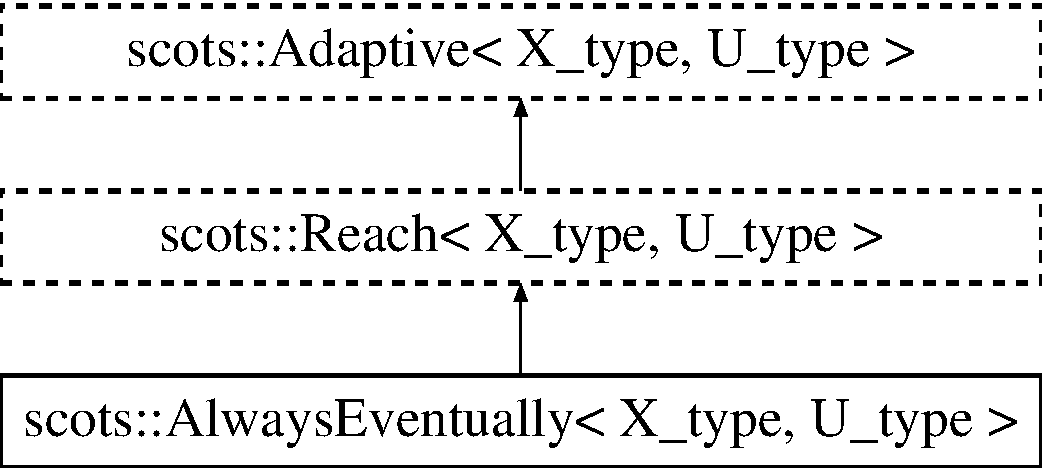
\includegraphics[height=3.000000cm]{classscots_1_1AlwaysEventually}
\end{center}
\end{figure}
\subsection*{Public Member Functions}
\begin{DoxyCompactItemize}
\item 
\hyperlink{classscots_1_1AlwaysEventually_a9a84a1c19b7ca2d26507247e47d3d95a}{Always\+Eventually} (int dimX, double $\ast$lbX, double $\ast$ubX, double $\ast$etaX, double tau, int dimU, double $\ast$lbU, double $\ast$ubU, double $\ast$etaU, double $\ast$eta\+Ratio, double tau\+Ratio, int nint, int num\+Abs, int read\+XX, int read\+Abs, char $\ast$log\+File)
\item 
\hyperlink{classscots_1_1AlwaysEventually_aa3d060f750bf82b5a41afdf7d925c3bb}{$\sim$\+Always\+Eventually} ()
\item 
int \hyperlink{classscots_1_1AlwaysEventually_a2428c979a09a3aa7efeed53059098bbc}{always\+Eventually} (int start\+Abs, int min\+To\+Go\+Coarser, int min\+To\+Be\+Valid, int verbose=1)
\end{DoxyCompactItemize}
\subsection*{Additional Inherited Members}


\subsection{Detailed Description}
\subsubsection*{template$<$class X\+\_\+type, class U\+\_\+type$>$\newline
class scots\+::\+Always\+Eventually$<$ X\+\_\+type, U\+\_\+type $>$}

A class (derived from base \hyperlink{classscots_1_1Adaptive}{Adaptive}) that does adaptive multiscale abstraction-\/based synthesis for an always-\/eventually specification. 

\subsection{Constructor \& Destructor Documentation}
\mbox{\Hypertarget{classscots_1_1AlwaysEventually_a9a84a1c19b7ca2d26507247e47d3d95a}\label{classscots_1_1AlwaysEventually_a9a84a1c19b7ca2d26507247e47d3d95a}} 
\index{scots\+::\+Always\+Eventually@{scots\+::\+Always\+Eventually}!Always\+Eventually@{Always\+Eventually}}
\index{Always\+Eventually@{Always\+Eventually}!scots\+::\+Always\+Eventually@{scots\+::\+Always\+Eventually}}
\subsubsection{\texorpdfstring{Always\+Eventually()}{AlwaysEventually()}}
{\footnotesize\ttfamily template$<$class X\+\_\+type , class U\+\_\+type $>$ \\
\hyperlink{classscots_1_1AlwaysEventually}{scots\+::\+Always\+Eventually}$<$ X\+\_\+type, U\+\_\+type $>$\+::\hyperlink{classscots_1_1AlwaysEventually}{Always\+Eventually} (\begin{DoxyParamCaption}\item[{int}]{dimX,  }\item[{double $\ast$}]{lbX,  }\item[{double $\ast$}]{ubX,  }\item[{double $\ast$}]{etaX,  }\item[{double}]{tau,  }\item[{int}]{dimU,  }\item[{double $\ast$}]{lbU,  }\item[{double $\ast$}]{ubU,  }\item[{double $\ast$}]{etaU,  }\item[{double $\ast$}]{eta\+Ratio,  }\item[{double}]{tau\+Ratio,  }\item[{int}]{nint,  }\item[{int}]{num\+Abs,  }\item[{int}]{read\+XX,  }\item[{int}]{read\+Abs,  }\item[{char $\ast$}]{log\+File }\end{DoxyParamCaption})\hspace{0.3cm}{\ttfamily [inline]}}

Constructor for an \hyperlink{classscots_1_1AlwaysEventually}{Always\+Eventually} object. \mbox{\Hypertarget{classscots_1_1AlwaysEventually_aa3d060f750bf82b5a41afdf7d925c3bb}\label{classscots_1_1AlwaysEventually_aa3d060f750bf82b5a41afdf7d925c3bb}} 
\index{scots\+::\+Always\+Eventually@{scots\+::\+Always\+Eventually}!````~Always\+Eventually@{$\sim$\+Always\+Eventually}}
\index{````~Always\+Eventually@{$\sim$\+Always\+Eventually}!scots\+::\+Always\+Eventually@{scots\+::\+Always\+Eventually}}
\subsubsection{\texorpdfstring{$\sim$\+Always\+Eventually()}{~AlwaysEventually()}}
{\footnotesize\ttfamily template$<$class X\+\_\+type , class U\+\_\+type $>$ \\
\hyperlink{classscots_1_1AlwaysEventually}{scots\+::\+Always\+Eventually}$<$ X\+\_\+type, U\+\_\+type $>$\+::$\sim$\hyperlink{classscots_1_1AlwaysEventually}{Always\+Eventually} (\begin{DoxyParamCaption}{ }\end{DoxyParamCaption})\hspace{0.3cm}{\ttfamily [inline]}}

Deconstructor for an \hyperlink{classscots_1_1AlwaysEventually}{Always\+Eventually} object. 

\subsection{Member Function Documentation}
\mbox{\Hypertarget{classscots_1_1AlwaysEventually_a2428c979a09a3aa7efeed53059098bbc}\label{classscots_1_1AlwaysEventually_a2428c979a09a3aa7efeed53059098bbc}} 
\index{scots\+::\+Always\+Eventually@{scots\+::\+Always\+Eventually}!always\+Eventually@{always\+Eventually}}
\index{always\+Eventually@{always\+Eventually}!scots\+::\+Always\+Eventually@{scots\+::\+Always\+Eventually}}
\subsubsection{\texorpdfstring{always\+Eventually()}{alwaysEventually()}}
{\footnotesize\ttfamily template$<$class X\+\_\+type , class U\+\_\+type $>$ \\
int \hyperlink{classscots_1_1AlwaysEventually}{scots\+::\+Always\+Eventually}$<$ X\+\_\+type, U\+\_\+type $>$\+::always\+Eventually (\begin{DoxyParamCaption}\item[{int}]{start\+Abs,  }\item[{int}]{min\+To\+Go\+Coarser,  }\item[{int}]{min\+To\+Be\+Valid,  }\item[{int}]{verbose = {\ttfamily 1} }\end{DoxyParamCaption})\hspace{0.3cm}{\ttfamily [inline]}}

Writes, should they exist, a sequence of controller and controller domain B\+D\+Ds to directories \textquotesingle{}C\textquotesingle{} and \textquotesingle{}Z\textquotesingle{} respectively that satisfy the Buchi box-\/diamond (aka always-\/eventually) specification. Note\+: of the n resultant controllers in \textquotesingle{}C\textquotesingle{}, the n-\/1th, .., 1st controllers are to reach, and the nth controller is for when the system state is a goal state. 
\begin{DoxyParams}[1]{Parameters}
\mbox{\tt in}  & {\em start\+Abs} & 0-\/index of the abstraction to start with. \\
\hline
\mbox{\tt in}  & {\em min\+To\+Go\+Coarser} & Minimum number of growing fixed point iterations needed before an attempt to go to a coarser abstraction. \\
\hline
\mbox{\tt in}  & {\em min\+To\+Be\+Valid} & Minimum number of growing fixed point iterations needed before a controller is declared valid. \\
\hline
\mbox{\tt in}  & {\em verbose} & If 1, prints additional information during synthesis to the log file. \\
\hline
\end{DoxyParams}
\begin{DoxyReturn}{Returns}
1 if controller(s) satisfying specification is/are synthesized; 0 otherwise. 
\end{DoxyReturn}


The documentation for this class was generated from the following file\+:\begin{DoxyCompactItemize}
\item 
/home/kylehsu/\+S\+C\+O\+T\+S-\/\+Adaptive/bdd/\hyperlink{AlwaysEventually_8hh}{Always\+Eventually.\+hh}\end{DoxyCompactItemize}

\hypertarget{classscots_1_1Compare}{}\section{scots\+:\+:Compare$<$ X\+\_\+type, U\+\_\+type $>$ Class Template Reference}
\label{classscots_1_1Compare}\index{scots\+::\+Compare$<$ X\+\_\+type, U\+\_\+type $>$@{scots\+::\+Compare$<$ X\+\_\+type, U\+\_\+type $>$}}


A class that provides comparison using basic S\+C\+O\+TS.  




{\ttfamily \#include $<$Compare.\+hh$>$}

\subsection*{Public Member Functions}
\begin{DoxyCompactItemize}
\item 
\hyperlink{classscots_1_1Compare_a41fa2b26a7292b46edd3dfc7a6f8c5ee}{Compare} (int dimX, double $\ast$lbX, double $\ast$ubX, double $\ast$etaX, double tau, int dimU, double $\ast$lbU, double $\ast$ubU, double $\ast$etaU, double $\ast$eta\+Ratio, double tau\+Ratio, int nint, int num\+Abs, int read\+Ab, char $\ast$log\+File)
\item 
\hyperlink{classscots_1_1Compare_abcd6b6626afb98b977a1c9d64ef438f2}{$\sim$\+Compare} ()
\item 
void \hyperlink{classscots_1_1Compare_aa96846be5c881576f5add5ce32f7fe8a}{save\+Verify\+Reach} ()
\item 
{\footnotesize template$<$class G\+\_\+type , class I\+\_\+type , class O\+\_\+type $>$ }\\void \hyperlink{classscots_1_1Compare_a4cb70ea51bb4778d92bd134c3b2ffc5e}{initialize\+Reach} (G\+\_\+type addG, I\+\_\+type addI, O\+\_\+type addO)
\item 
void \hyperlink{classscots_1_1Compare_a506b87a62b1adde561d725e9cc1315e9}{reach\+S\+C\+O\+TS} (int early\+Break, int verbose=1)
\item 
void \hyperlink{classscots_1_1Compare_afbc28a076ac3c620d4eae4b8af905877}{always\+Eventually\+S\+C\+O\+TS} ()
\item 
void \hyperlink{classscots_1_1Compare_a9e79295cd6f8c7eed65d29ca2667cff9}{save\+Verify\+Safe} ()
\item 
{\footnotesize template$<$class S\+\_\+type $>$ }\\void \hyperlink{classscots_1_1Compare_aec4ea9d5132711c734141bd9ed060752}{initialize\+Safe} (S\+\_\+type addS)
\item 
void \hyperlink{classscots_1_1Compare_ad54d4ddd0268b4a41e53f19d668ab8b0}{safe\+S\+C\+O\+TS} ()
\item 
{\footnotesize template$<$class sys\+\_\+type , class rad\+\_\+type $>$ }\\void \hyperlink{classscots_1_1Compare_a3bdf985c18d37edf8ee63ea00f6b2635}{compute\+Abstractions} (sys\+\_\+type sys\+Next, rad\+\_\+type rad\+Next)
\item 
{\footnotesize template$<$class msg\+\_\+type $>$ }\\void \hyperlink{classscots_1_1Compare_ae694b20dbe9ceb8db5f80508e7c65488}{error} (msg\+\_\+type msg)
\item 
void \hyperlink{classscots_1_1Compare_a4ed25bd656e43ea3693266843edb88d2}{print\+EtaX} (double $\ast$etaX, int dimX)
\item 
void \hyperlink{classscots_1_1Compare_a9f062bcfa755da8ba004045cb9605ab5}{print\+Tau} (double tau)
\end{DoxyCompactItemize}
\subsection*{Public Attributes}
\begin{DoxyCompactItemize}
\item 
Cudd \hyperlink{classscots_1_1Compare_a330d650aa232026ba22f43aa81974af9}{ddmgr\+\_\+}
\item 
int \hyperlink{classscots_1_1Compare_ad18456a4cc253ae0d300cda74517e64b}{read\+Ab\+\_\+}
\item 
Symbolic\+Set $\ast$ \hyperlink{classscots_1_1Compare_a4d0bb95aefd7ffeda946bd79a8170825}{X\+\_\+}
\item 
Symbolic\+Set $\ast$ \hyperlink{classscots_1_1Compare_a1a7d912c19ff01269353ec705a257ad6}{G\+\_\+}
\item 
Symbolic\+Set $\ast$ \hyperlink{classscots_1_1Compare_a32b383c4e137a371859fdee22c165486}{I\+\_\+}
\item 
Symbolic\+Set $\ast$ \hyperlink{classscots_1_1Compare_a5dd50527db402893630c209d05be4ef0}{O\+\_\+}
\item 
Symbolic\+Set $\ast$ \hyperlink{classscots_1_1Compare_a3f1ba24992e2dfe24358087aeecb5a75}{X2\+\_\+}
\item 
Symbolic\+Set $\ast$ \hyperlink{classscots_1_1Compare_ac341e6c2534e4bb4ab248cc767c33b8d}{U\+\_\+}
\item 
Symbolic\+Set $\ast$ \hyperlink{classscots_1_1Compare_a1ffd2853abc9ab09cfb8983b3664ab1b}{C\+\_\+}
\item 
Symbolic\+Set $\ast$ \hyperlink{classscots_1_1Compare_aeb0830d94286ae12672cf1ea183afb1d}{T\+\_\+}
\item 
Symbolic\+Set $\ast$ \hyperlink{classscots_1_1Compare_a2512f264f83a21365693bbd506b9e7a2}{S\+\_\+}
\item 
Symbolic\+Set $\ast$ \hyperlink{classscots_1_1Compare_ae1a8d5e076e059cda7124581dc3d05ab}{Z\+\_\+}
\item 
Ode\+Solver $\ast$ \hyperlink{classscots_1_1Compare_aa42864e8794631891d01f0367e1db277}{solver\+\_\+}
\item 
Symbolic\+Model\+Growth\+Bound$<$ X\+\_\+type, U\+\_\+type $>$ $\ast$ \hyperlink{classscots_1_1Compare_a0ec2c4c168dc46f79616a393c1cda103}{Ab\+\_\+}
\item 
int \hyperlink{classscots_1_1Compare_ae036e8066fed2391f333c8f64282f12e}{stage\+\_\+}
\end{DoxyCompactItemize}


\subsection{Detailed Description}
\subsubsection*{template$<$class X\+\_\+type, class U\+\_\+type$>$\newline
class scots\+::\+Compare$<$ X\+\_\+type, U\+\_\+type $>$}

A class that provides comparison using basic S\+C\+O\+TS. 

\subsection{Constructor \& Destructor Documentation}
\mbox{\Hypertarget{classscots_1_1Compare_a41fa2b26a7292b46edd3dfc7a6f8c5ee}\label{classscots_1_1Compare_a41fa2b26a7292b46edd3dfc7a6f8c5ee}} 
\index{scots\+::\+Compare@{scots\+::\+Compare}!Compare@{Compare}}
\index{Compare@{Compare}!scots\+::\+Compare@{scots\+::\+Compare}}
\subsubsection{\texorpdfstring{Compare()}{Compare()}}
{\footnotesize\ttfamily template$<$class X\+\_\+type , class U\+\_\+type $>$ \\
\hyperlink{classscots_1_1Compare}{scots\+::\+Compare}$<$ X\+\_\+type, U\+\_\+type $>$\+::\hyperlink{classscots_1_1Compare}{Compare} (\begin{DoxyParamCaption}\item[{int}]{dimX,  }\item[{double $\ast$}]{lbX,  }\item[{double $\ast$}]{ubX,  }\item[{double $\ast$}]{etaX,  }\item[{double}]{tau,  }\item[{int}]{dimU,  }\item[{double $\ast$}]{lbU,  }\item[{double $\ast$}]{ubU,  }\item[{double $\ast$}]{etaU,  }\item[{double $\ast$}]{eta\+Ratio,  }\item[{double}]{tau\+Ratio,  }\item[{int}]{nint,  }\item[{int}]{num\+Abs,  }\item[{int}]{read\+Ab,  }\item[{char $\ast$}]{log\+File }\end{DoxyParamCaption})\hspace{0.3cm}{\ttfamily [inline]}}

Constructor for a \hyperlink{classscots_1_1Compare}{Compare} object. 
\begin{DoxyParams}[1]{Parameters}
\mbox{\tt in}  & {\em dimX} & Dimensionality of the state space. \\
\hline
\mbox{\tt in}  & {\em lbX} & Lowermost grid point of the state space. \\
\hline
\mbox{\tt in}  & {\em ubX} & Uppermost grid point of the state space. \\
\hline
\mbox{\tt in}  & {\em etaX} & Grid spacing of the state space. \\
\hline
\mbox{\tt in}  & {\em tau} & Time step. \\
\hline
\mbox{\tt in}  & {\em dimU} & Dimensionality of the input space. \\
\hline
\mbox{\tt in}  & {\em lbU} & Lowermost grid point of the input space. \\
\hline
\mbox{\tt in}  & {\em ubU} & Uppermost grid point of the input space. \\
\hline
\mbox{\tt in}  & {\em etaU} & Grid spacing of the input space. \\
\hline
\mbox{\tt in}  & {\em eta\+Ratio} & (\hyperlink{Adaptive_8hh}{Adaptive.\+hh}) Ratio between grid spacings of the input space in consecutive abstractions. \\
\hline
\mbox{\tt in}  & {\em tau\+Ratio} & (\hyperlink{Adaptive_8hh}{Adaptive.\+hh}) Ratio between time steps of consecutive abstractions. \\
\hline
\mbox{\tt in}  & {\em nint} & Number of sub-\/intervals in O\+DE solving per time step. \\
\hline
\mbox{\tt in}  & {\em num\+Abs} & (\hyperlink{Adaptive_8hh}{Adaptive.\+hh}) Number of abstractions. \\
\hline
\mbox{\tt in}  & {\em read\+Ab} & Whether transition relation should constructed (0) or read from file (1). \\
\hline
\mbox{\tt in}  & {\em log\+File} & Filename of program log. \\
\hline
\end{DoxyParams}
\mbox{\Hypertarget{classscots_1_1Compare_abcd6b6626afb98b977a1c9d64ef438f2}\label{classscots_1_1Compare_abcd6b6626afb98b977a1c9d64ef438f2}} 
\index{scots\+::\+Compare@{scots\+::\+Compare}!````~Compare@{$\sim$\+Compare}}
\index{````~Compare@{$\sim$\+Compare}!scots\+::\+Compare@{scots\+::\+Compare}}
\subsubsection{\texorpdfstring{$\sim$\+Compare()}{~Compare()}}
{\footnotesize\ttfamily template$<$class X\+\_\+type , class U\+\_\+type $>$ \\
\hyperlink{classscots_1_1Compare}{scots\+::\+Compare}$<$ X\+\_\+type, U\+\_\+type $>$\+::$\sim$\hyperlink{classscots_1_1Compare}{Compare} (\begin{DoxyParamCaption}{ }\end{DoxyParamCaption})\hspace{0.3cm}{\ttfamily [inline]}}

Destructor for a \hyperlink{classscots_1_1Compare}{Compare} object. 

\subsection{Member Function Documentation}
\mbox{\Hypertarget{classscots_1_1Compare_afbc28a076ac3c620d4eae4b8af905877}\label{classscots_1_1Compare_afbc28a076ac3c620d4eae4b8af905877}} 
\index{scots\+::\+Compare@{scots\+::\+Compare}!always\+Eventually\+S\+C\+O\+TS@{always\+Eventually\+S\+C\+O\+TS}}
\index{always\+Eventually\+S\+C\+O\+TS@{always\+Eventually\+S\+C\+O\+TS}!scots\+::\+Compare@{scots\+::\+Compare}}
\subsubsection{\texorpdfstring{always\+Eventually\+S\+C\+O\+T\+S()}{alwaysEventuallySCOTS()}}
{\footnotesize\ttfamily template$<$class X\+\_\+type , class U\+\_\+type $>$ \\
void \hyperlink{classscots_1_1Compare}{scots\+::\+Compare}$<$ X\+\_\+type, U\+\_\+type $>$\+::always\+Eventually\+S\+C\+O\+TS (\begin{DoxyParamCaption}{ }\end{DoxyParamCaption})\hspace{0.3cm}{\ttfamily [inline]}}

Implementation of always-\/eventually using functions in a S\+C\+O\+T\+S\+::\+Fixed\+Point object. For comparison with the \hyperlink{classscots_1_1Adaptive}{Adaptive} version. \mbox{\Hypertarget{classscots_1_1Compare_a3bdf985c18d37edf8ee63ea00f6b2635}\label{classscots_1_1Compare_a3bdf985c18d37edf8ee63ea00f6b2635}} 
\index{scots\+::\+Compare@{scots\+::\+Compare}!compute\+Abstractions@{compute\+Abstractions}}
\index{compute\+Abstractions@{compute\+Abstractions}!scots\+::\+Compare@{scots\+::\+Compare}}
\subsubsection{\texorpdfstring{compute\+Abstractions()}{computeAbstractions()}}
{\footnotesize\ttfamily template$<$class X\+\_\+type , class U\+\_\+type $>$ \\
template$<$class sys\+\_\+type , class rad\+\_\+type $>$ \\
void \hyperlink{classscots_1_1Compare}{scots\+::\+Compare}$<$ X\+\_\+type, U\+\_\+type $>$\+::compute\+Abstractions (\begin{DoxyParamCaption}\item[{sys\+\_\+type}]{sys\+Next,  }\item[{rad\+\_\+type}]{rad\+Next }\end{DoxyParamCaption})\hspace{0.3cm}{\ttfamily [inline]}}

Initializes Symbolic\+Model\+Growth\+Bound objects for each abstraction as well as Ts\+\_\+, T\+Ts\+\_\+ for use in the fixed points. 
\begin{DoxyParams}[1]{Parameters}
\mbox{\tt in}  & {\em sys\+Next} & Function pointer to equation that evolves system state. \\
\hline
\mbox{\tt in}  & {\em rad\+Next} & Function pointer to equation that computes growth bound. \\
\hline
\end{DoxyParams}
\mbox{\Hypertarget{classscots_1_1Compare_ae694b20dbe9ceb8db5f80508e7c65488}\label{classscots_1_1Compare_ae694b20dbe9ceb8db5f80508e7c65488}} 
\index{scots\+::\+Compare@{scots\+::\+Compare}!error@{error}}
\index{error@{error}!scots\+::\+Compare@{scots\+::\+Compare}}
\subsubsection{\texorpdfstring{error()}{error()}}
{\footnotesize\ttfamily template$<$class X\+\_\+type , class U\+\_\+type $>$ \\
template$<$class msg\+\_\+type $>$ \\
void \hyperlink{classscots_1_1Compare}{scots\+::\+Compare}$<$ X\+\_\+type, U\+\_\+type $>$\+::error (\begin{DoxyParamCaption}\item[{msg\+\_\+type}]{msg }\end{DoxyParamCaption})\hspace{0.3cm}{\ttfamily [inline]}}

Throws a logic error along with specified message and closes the log file. 
\begin{DoxyParams}[1]{Parameters}
\mbox{\tt in}  & {\em msg} & Error message to log to file. \\
\hline
\end{DoxyParams}
\mbox{\Hypertarget{classscots_1_1Compare_a4cb70ea51bb4778d92bd134c3b2ffc5e}\label{classscots_1_1Compare_a4cb70ea51bb4778d92bd134c3b2ffc5e}} 
\index{scots\+::\+Compare@{scots\+::\+Compare}!initialize\+Reach@{initialize\+Reach}}
\index{initialize\+Reach@{initialize\+Reach}!scots\+::\+Compare@{scots\+::\+Compare}}
\subsubsection{\texorpdfstring{initialize\+Reach()}{initializeReach()}}
{\footnotesize\ttfamily template$<$class X\+\_\+type , class U\+\_\+type $>$ \\
template$<$class G\+\_\+type , class I\+\_\+type , class O\+\_\+type $>$ \\
void \hyperlink{classscots_1_1Compare}{scots\+::\+Compare}$<$ X\+\_\+type, U\+\_\+type $>$\+::initialize\+Reach (\begin{DoxyParamCaption}\item[{G\+\_\+type}]{addG,  }\item[{I\+\_\+type}]{addI,  }\item[{O\+\_\+type}]{addO }\end{DoxyParamCaption})\hspace{0.3cm}{\ttfamily [inline]}}

Initializes objects specific to the following specifications\+: always-\/eventually, reach-\/while-\/avoid. 
\begin{DoxyParams}[1]{Parameters}
\mbox{\tt in}  & {\em addG} & Function pointer specifying the points that should be added to the goal set. \\
\hline
\mbox{\tt in}  & {\em addI} & Function pointer specifying the points that should be added to the initial set. \\
\hline
\mbox{\tt in}  & {\em addO} & Function pointer specifying the points that should be added to the obstacle set. \\
\hline
\end{DoxyParams}
\mbox{\Hypertarget{classscots_1_1Compare_aec4ea9d5132711c734141bd9ed060752}\label{classscots_1_1Compare_aec4ea9d5132711c734141bd9ed060752}} 
\index{scots\+::\+Compare@{scots\+::\+Compare}!initialize\+Safe@{initialize\+Safe}}
\index{initialize\+Safe@{initialize\+Safe}!scots\+::\+Compare@{scots\+::\+Compare}}
\subsubsection{\texorpdfstring{initialize\+Safe()}{initializeSafe()}}
{\footnotesize\ttfamily template$<$class X\+\_\+type , class U\+\_\+type $>$ \\
template$<$class S\+\_\+type $>$ \\
void \hyperlink{classscots_1_1Compare}{scots\+::\+Compare}$<$ X\+\_\+type, U\+\_\+type $>$\+::initialize\+Safe (\begin{DoxyParamCaption}\item[{S\+\_\+type}]{addS }\end{DoxyParamCaption})\hspace{0.3cm}{\ttfamily [inline]}}

Initializes objects specific to the following specifications\+: safe. 
\begin{DoxyParams}[1]{Parameters}
\mbox{\tt in}  & {\em addS} & Function pointer specifying the points that should be added to the potential safe set. \\
\hline
\end{DoxyParams}
\mbox{\Hypertarget{classscots_1_1Compare_a4ed25bd656e43ea3693266843edb88d2}\label{classscots_1_1Compare_a4ed25bd656e43ea3693266843edb88d2}} 
\index{scots\+::\+Compare@{scots\+::\+Compare}!print\+EtaX@{print\+EtaX}}
\index{print\+EtaX@{print\+EtaX}!scots\+::\+Compare@{scots\+::\+Compare}}
\subsubsection{\texorpdfstring{print\+Eta\+X()}{printEtaX()}}
{\footnotesize\ttfamily template$<$class X\+\_\+type , class U\+\_\+type $>$ \\
void \hyperlink{classscots_1_1Compare}{scots\+::\+Compare}$<$ X\+\_\+type, U\+\_\+type $>$\+::print\+EtaX (\begin{DoxyParamCaption}\item[{double $\ast$}]{etaX,  }\item[{int}]{dimX }\end{DoxyParamCaption})\hspace{0.3cm}{\ttfamily [inline]}}

Prints information regarding the abstractions\textquotesingle{} grid parameters to the log file. \mbox{\Hypertarget{classscots_1_1Compare_a9f062bcfa755da8ba004045cb9605ab5}\label{classscots_1_1Compare_a9f062bcfa755da8ba004045cb9605ab5}} 
\index{scots\+::\+Compare@{scots\+::\+Compare}!print\+Tau@{print\+Tau}}
\index{print\+Tau@{print\+Tau}!scots\+::\+Compare@{scots\+::\+Compare}}
\subsubsection{\texorpdfstring{print\+Tau()}{printTau()}}
{\footnotesize\ttfamily template$<$class X\+\_\+type , class U\+\_\+type $>$ \\
void \hyperlink{classscots_1_1Compare}{scots\+::\+Compare}$<$ X\+\_\+type, U\+\_\+type $>$\+::print\+Tau (\begin{DoxyParamCaption}\item[{double}]{tau }\end{DoxyParamCaption})\hspace{0.3cm}{\ttfamily [inline]}}

Prints information regarding the time sampling parameter to the log file. \mbox{\Hypertarget{classscots_1_1Compare_a506b87a62b1adde561d725e9cc1315e9}\label{classscots_1_1Compare_a506b87a62b1adde561d725e9cc1315e9}} 
\index{scots\+::\+Compare@{scots\+::\+Compare}!reach\+S\+C\+O\+TS@{reach\+S\+C\+O\+TS}}
\index{reach\+S\+C\+O\+TS@{reach\+S\+C\+O\+TS}!scots\+::\+Compare@{scots\+::\+Compare}}
\subsubsection{\texorpdfstring{reach\+S\+C\+O\+T\+S()}{reachSCOTS()}}
{\footnotesize\ttfamily template$<$class X\+\_\+type , class U\+\_\+type $>$ \\
void \hyperlink{classscots_1_1Compare}{scots\+::\+Compare}$<$ X\+\_\+type, U\+\_\+type $>$\+::reach\+S\+C\+O\+TS (\begin{DoxyParamCaption}\item[{int}]{early\+Break,  }\item[{int}]{verbose = {\ttfamily 1} }\end{DoxyParamCaption})\hspace{0.3cm}{\ttfamily [inline]}}

Implementation of reachability using only a scots\+::\+Fixed\+Point object. For comparison with the \hyperlink{classscots_1_1Adaptive}{Adaptive} version. 
\begin{DoxyParams}[1]{Parameters}
\mbox{\tt in}  & {\em early\+Break} & If 1, the synthesis ends as soon as I meets the domain of C. \\
\hline
\mbox{\tt in}  & {\em verbose} & If 1, prints additional information during synthesis to the log file. \\
\hline
\end{DoxyParams}
\mbox{\Hypertarget{classscots_1_1Compare_ad54d4ddd0268b4a41e53f19d668ab8b0}\label{classscots_1_1Compare_ad54d4ddd0268b4a41e53f19d668ab8b0}} 
\index{scots\+::\+Compare@{scots\+::\+Compare}!safe\+S\+C\+O\+TS@{safe\+S\+C\+O\+TS}}
\index{safe\+S\+C\+O\+TS@{safe\+S\+C\+O\+TS}!scots\+::\+Compare@{scots\+::\+Compare}}
\subsubsection{\texorpdfstring{safe\+S\+C\+O\+T\+S()}{safeSCOTS()}}
{\footnotesize\ttfamily template$<$class X\+\_\+type , class U\+\_\+type $>$ \\
void \hyperlink{classscots_1_1Compare}{scots\+::\+Compare}$<$ X\+\_\+type, U\+\_\+type $>$\+::safe\+S\+C\+O\+TS (\begin{DoxyParamCaption}{ }\end{DoxyParamCaption})\hspace{0.3cm}{\ttfamily [inline]}}

Implementation of safety using functions in a S\+C\+O\+T\+S\+::\+Fixed\+Point object. For comparison with the \hyperlink{classscots_1_1Adaptive}{Adaptive} version. \mbox{\Hypertarget{classscots_1_1Compare_aa96846be5c881576f5add5ce32f7fe8a}\label{classscots_1_1Compare_aa96846be5c881576f5add5ce32f7fe8a}} 
\index{scots\+::\+Compare@{scots\+::\+Compare}!save\+Verify\+Reach@{save\+Verify\+Reach}}
\index{save\+Verify\+Reach@{save\+Verify\+Reach}!scots\+::\+Compare@{scots\+::\+Compare}}
\subsubsection{\texorpdfstring{save\+Verify\+Reach()}{saveVerifyReach()}}
{\footnotesize\ttfamily template$<$class X\+\_\+type , class U\+\_\+type $>$ \\
void \hyperlink{classscots_1_1Compare}{scots\+::\+Compare}$<$ X\+\_\+type, U\+\_\+type $>$\+::save\+Verify\+Reach (\begin{DoxyParamCaption}{ }\end{DoxyParamCaption})\hspace{0.3cm}{\ttfamily [inline]}}

Saves and prints to console some information related to the reachability/always-\/eventually specification. \mbox{\Hypertarget{classscots_1_1Compare_a9e79295cd6f8c7eed65d29ca2667cff9}\label{classscots_1_1Compare_a9e79295cd6f8c7eed65d29ca2667cff9}} 
\index{scots\+::\+Compare@{scots\+::\+Compare}!save\+Verify\+Safe@{save\+Verify\+Safe}}
\index{save\+Verify\+Safe@{save\+Verify\+Safe}!scots\+::\+Compare@{scots\+::\+Compare}}
\subsubsection{\texorpdfstring{save\+Verify\+Safe()}{saveVerifySafe()}}
{\footnotesize\ttfamily template$<$class X\+\_\+type , class U\+\_\+type $>$ \\
void \hyperlink{classscots_1_1Compare}{scots\+::\+Compare}$<$ X\+\_\+type, U\+\_\+type $>$\+::save\+Verify\+Safe (\begin{DoxyParamCaption}{ }\end{DoxyParamCaption})\hspace{0.3cm}{\ttfamily [inline]}}

Saves and prints to log file some information related to the safety specification. 

\subsection{Member Data Documentation}
\mbox{\Hypertarget{classscots_1_1Compare_a0ec2c4c168dc46f79616a393c1cda103}\label{classscots_1_1Compare_a0ec2c4c168dc46f79616a393c1cda103}} 
\index{scots\+::\+Compare@{scots\+::\+Compare}!Ab\+\_\+@{Ab\+\_\+}}
\index{Ab\+\_\+@{Ab\+\_\+}!scots\+::\+Compare@{scots\+::\+Compare}}
\subsubsection{\texorpdfstring{Ab\+\_\+}{Ab\_}}
{\footnotesize\ttfamily template$<$class X\+\_\+type , class U\+\_\+type $>$ \\
Symbolic\+Model\+Growth\+Bound$<$X\+\_\+type, U\+\_\+type$>$$\ast$ \hyperlink{classscots_1_1Compare}{scots\+::\+Compare}$<$ X\+\_\+type, U\+\_\+type $>$\+::Ab\+\_\+}

Abstraction containing the transition relation. \mbox{\Hypertarget{classscots_1_1Compare_a1ffd2853abc9ab09cfb8983b3664ab1b}\label{classscots_1_1Compare_a1ffd2853abc9ab09cfb8983b3664ab1b}} 
\index{scots\+::\+Compare@{scots\+::\+Compare}!C\+\_\+@{C\+\_\+}}
\index{C\+\_\+@{C\+\_\+}!scots\+::\+Compare@{scots\+::\+Compare}}
\subsubsection{\texorpdfstring{C\+\_\+}{C\_}}
{\footnotesize\ttfamily template$<$class X\+\_\+type , class U\+\_\+type $>$ \\
Symbolic\+Set$\ast$ \hyperlink{classscots_1_1Compare}{scots\+::\+Compare}$<$ X\+\_\+type, U\+\_\+type $>$\+::C\+\_\+}

Controller. \mbox{\Hypertarget{classscots_1_1Compare_a330d650aa232026ba22f43aa81974af9}\label{classscots_1_1Compare_a330d650aa232026ba22f43aa81974af9}} 
\index{scots\+::\+Compare@{scots\+::\+Compare}!ddmgr\+\_\+@{ddmgr\+\_\+}}
\index{ddmgr\+\_\+@{ddmgr\+\_\+}!scots\+::\+Compare@{scots\+::\+Compare}}
\subsubsection{\texorpdfstring{ddmgr\+\_\+}{ddmgr\_}}
{\footnotesize\ttfamily template$<$class X\+\_\+type , class U\+\_\+type $>$ \\
Cudd \hyperlink{classscots_1_1Compare}{scots\+::\+Compare}$<$ X\+\_\+type, U\+\_\+type $>$\+::ddmgr\+\_\+}

A single manager object common to all B\+D\+Ds used in the program. \mbox{\Hypertarget{classscots_1_1Compare_a1a7d912c19ff01269353ec705a257ad6}\label{classscots_1_1Compare_a1a7d912c19ff01269353ec705a257ad6}} 
\index{scots\+::\+Compare@{scots\+::\+Compare}!G\+\_\+@{G\+\_\+}}
\index{G\+\_\+@{G\+\_\+}!scots\+::\+Compare@{scots\+::\+Compare}}
\subsubsection{\texorpdfstring{G\+\_\+}{G\_}}
{\footnotesize\ttfamily template$<$class X\+\_\+type , class U\+\_\+type $>$ \\
Symbolic\+Set$\ast$ \hyperlink{classscots_1_1Compare}{scots\+::\+Compare}$<$ X\+\_\+type, U\+\_\+type $>$\+::G\+\_\+}

Instance of $\ast$\+X\+\_\+ containing goal states. \mbox{\Hypertarget{classscots_1_1Compare_a32b383c4e137a371859fdee22c165486}\label{classscots_1_1Compare_a32b383c4e137a371859fdee22c165486}} 
\index{scots\+::\+Compare@{scots\+::\+Compare}!I\+\_\+@{I\+\_\+}}
\index{I\+\_\+@{I\+\_\+}!scots\+::\+Compare@{scots\+::\+Compare}}
\subsubsection{\texorpdfstring{I\+\_\+}{I\_}}
{\footnotesize\ttfamily template$<$class X\+\_\+type , class U\+\_\+type $>$ \\
Symbolic\+Set$\ast$ \hyperlink{classscots_1_1Compare}{scots\+::\+Compare}$<$ X\+\_\+type, U\+\_\+type $>$\+::I\+\_\+}

Instance of $\ast$\+X\+\_\+ containing initial states. \mbox{\Hypertarget{classscots_1_1Compare_a5dd50527db402893630c209d05be4ef0}\label{classscots_1_1Compare_a5dd50527db402893630c209d05be4ef0}} 
\index{scots\+::\+Compare@{scots\+::\+Compare}!O\+\_\+@{O\+\_\+}}
\index{O\+\_\+@{O\+\_\+}!scots\+::\+Compare@{scots\+::\+Compare}}
\subsubsection{\texorpdfstring{O\+\_\+}{O\_}}
{\footnotesize\ttfamily template$<$class X\+\_\+type , class U\+\_\+type $>$ \\
Symbolic\+Set$\ast$ \hyperlink{classscots_1_1Compare}{scots\+::\+Compare}$<$ X\+\_\+type, U\+\_\+type $>$\+::O\+\_\+}

Instance of $\ast$\+X\+\_\+ containing unsafe (obstacle) states. \mbox{\Hypertarget{classscots_1_1Compare_ad18456a4cc253ae0d300cda74517e64b}\label{classscots_1_1Compare_ad18456a4cc253ae0d300cda74517e64b}} 
\index{scots\+::\+Compare@{scots\+::\+Compare}!read\+Ab\+\_\+@{read\+Ab\+\_\+}}
\index{read\+Ab\+\_\+@{read\+Ab\+\_\+}!scots\+::\+Compare@{scots\+::\+Compare}}
\subsubsection{\texorpdfstring{read\+Ab\+\_\+}{readAb\_}}
{\footnotesize\ttfamily template$<$class X\+\_\+type , class U\+\_\+type $>$ \\
int \hyperlink{classscots_1_1Compare}{scots\+::\+Compare}$<$ X\+\_\+type, U\+\_\+type $>$\+::read\+Ab\+\_\+}

Whether transition relation is computed or read from file. \mbox{\Hypertarget{classscots_1_1Compare_a2512f264f83a21365693bbd506b9e7a2}\label{classscots_1_1Compare_a2512f264f83a21365693bbd506b9e7a2}} 
\index{scots\+::\+Compare@{scots\+::\+Compare}!S\+\_\+@{S\+\_\+}}
\index{S\+\_\+@{S\+\_\+}!scots\+::\+Compare@{scots\+::\+Compare}}
\subsubsection{\texorpdfstring{S\+\_\+}{S\_}}
{\footnotesize\ttfamily template$<$class X\+\_\+type , class U\+\_\+type $>$ \\
Symbolic\+Set$\ast$ \hyperlink{classscots_1_1Compare}{scots\+::\+Compare}$<$ X\+\_\+type, U\+\_\+type $>$\+::S\+\_\+}

Instance of $\ast$\+X\+\_\+ containing possible safe states. \mbox{\Hypertarget{classscots_1_1Compare_aa42864e8794631891d01f0367e1db277}\label{classscots_1_1Compare_aa42864e8794631891d01f0367e1db277}} 
\index{scots\+::\+Compare@{scots\+::\+Compare}!solver\+\_\+@{solver\+\_\+}}
\index{solver\+\_\+@{solver\+\_\+}!scots\+::\+Compare@{scots\+::\+Compare}}
\subsubsection{\texorpdfstring{solver\+\_\+}{solver\_}}
{\footnotesize\ttfamily template$<$class X\+\_\+type , class U\+\_\+type $>$ \\
Ode\+Solver$\ast$ \hyperlink{classscots_1_1Compare}{scots\+::\+Compare}$<$ X\+\_\+type, U\+\_\+type $>$\+::solver\+\_\+}

O\+DE solver (Runge-\/\+Katta approximation) for an abstraction time step. \mbox{\Hypertarget{classscots_1_1Compare_ae036e8066fed2391f333c8f64282f12e}\label{classscots_1_1Compare_ae036e8066fed2391f333c8f64282f12e}} 
\index{scots\+::\+Compare@{scots\+::\+Compare}!stage\+\_\+@{stage\+\_\+}}
\index{stage\+\_\+@{stage\+\_\+}!scots\+::\+Compare@{scots\+::\+Compare}}
\subsubsection{\texorpdfstring{stage\+\_\+}{stage\_}}
{\footnotesize\ttfamily template$<$class X\+\_\+type , class U\+\_\+type $>$ \\
int \hyperlink{classscots_1_1Compare}{scots\+::\+Compare}$<$ X\+\_\+type, U\+\_\+type $>$\+::stage\+\_\+}

Helps ensure user calls methods in correct order. \mbox{\Hypertarget{classscots_1_1Compare_aeb0830d94286ae12672cf1ea183afb1d}\label{classscots_1_1Compare_aeb0830d94286ae12672cf1ea183afb1d}} 
\index{scots\+::\+Compare@{scots\+::\+Compare}!T\+\_\+@{T\+\_\+}}
\index{T\+\_\+@{T\+\_\+}!scots\+::\+Compare@{scots\+::\+Compare}}
\subsubsection{\texorpdfstring{T\+\_\+}{T\_}}
{\footnotesize\ttfamily template$<$class X\+\_\+type , class U\+\_\+type $>$ \\
Symbolic\+Set$\ast$ \hyperlink{classscots_1_1Compare}{scots\+::\+Compare}$<$ X\+\_\+type, U\+\_\+type $>$\+::T\+\_\+}

Transition relation. \mbox{\Hypertarget{classscots_1_1Compare_ac341e6c2534e4bb4ab248cc767c33b8d}\label{classscots_1_1Compare_ac341e6c2534e4bb4ab248cc767c33b8d}} 
\index{scots\+::\+Compare@{scots\+::\+Compare}!U\+\_\+@{U\+\_\+}}
\index{U\+\_\+@{U\+\_\+}!scots\+::\+Compare@{scots\+::\+Compare}}
\subsubsection{\texorpdfstring{U\+\_\+}{U\_}}
{\footnotesize\ttfamily template$<$class X\+\_\+type , class U\+\_\+type $>$ \\
Symbolic\+Set$\ast$ \hyperlink{classscots_1_1Compare}{scots\+::\+Compare}$<$ X\+\_\+type, U\+\_\+type $>$\+::U\+\_\+}

The input space abstraction. \mbox{\Hypertarget{classscots_1_1Compare_a3f1ba24992e2dfe24358087aeecb5a75}\label{classscots_1_1Compare_a3f1ba24992e2dfe24358087aeecb5a75}} 
\index{scots\+::\+Compare@{scots\+::\+Compare}!X2\+\_\+@{X2\+\_\+}}
\index{X2\+\_\+@{X2\+\_\+}!scots\+::\+Compare@{scots\+::\+Compare}}
\subsubsection{\texorpdfstring{X2\+\_\+}{X2\_}}
{\footnotesize\ttfamily template$<$class X\+\_\+type , class U\+\_\+type $>$ \\
Symbolic\+Set$\ast$ \hyperlink{classscots_1_1Compare}{scots\+::\+Compare}$<$ X\+\_\+type, U\+\_\+type $>$\+::X2\+\_\+}

The \char`\"{}post\char`\"{} state space. \mbox{\Hypertarget{classscots_1_1Compare_a4d0bb95aefd7ffeda946bd79a8170825}\label{classscots_1_1Compare_a4d0bb95aefd7ffeda946bd79a8170825}} 
\index{scots\+::\+Compare@{scots\+::\+Compare}!X\+\_\+@{X\+\_\+}}
\index{X\+\_\+@{X\+\_\+}!scots\+::\+Compare@{scots\+::\+Compare}}
\subsubsection{\texorpdfstring{X\+\_\+}{X\_}}
{\footnotesize\ttfamily template$<$class X\+\_\+type , class U\+\_\+type $>$ \\
Symbolic\+Set$\ast$ \hyperlink{classscots_1_1Compare}{scots\+::\+Compare}$<$ X\+\_\+type, U\+\_\+type $>$\+::X\+\_\+}

State space. \mbox{\Hypertarget{classscots_1_1Compare_ae1a8d5e076e059cda7124581dc3d05ab}\label{classscots_1_1Compare_ae1a8d5e076e059cda7124581dc3d05ab}} 
\index{scots\+::\+Compare@{scots\+::\+Compare}!Z\+\_\+@{Z\+\_\+}}
\index{Z\+\_\+@{Z\+\_\+}!scots\+::\+Compare@{scots\+::\+Compare}}
\subsubsection{\texorpdfstring{Z\+\_\+}{Z\_}}
{\footnotesize\ttfamily template$<$class X\+\_\+type , class U\+\_\+type $>$ \\
Symbolic\+Set$\ast$ \hyperlink{classscots_1_1Compare}{scots\+::\+Compare}$<$ X\+\_\+type, U\+\_\+type $>$\+::Z\+\_\+}

Instance of $\ast$\+X\+\_\+ containing winning states. 

The documentation for this class was generated from the following file\+:\begin{DoxyCompactItemize}
\item 
/home/kylehsu/\+S\+C\+O\+T\+S-\/\+Adaptive/bdd/\hyperlink{Compare_8hh}{Compare.\+hh}\end{DoxyCompactItemize}

\hypertarget{classscots_1_1Reach}{}\section{scots\+:\+:Reach$<$ X\+\_\+type, U\+\_\+type $>$ Class Template Reference}
\label{classscots_1_1Reach}\index{scots\+::\+Reach$<$ X\+\_\+type, U\+\_\+type $>$@{scots\+::\+Reach$<$ X\+\_\+type, U\+\_\+type $>$}}


A class (derived from base \hyperlink{classscots_1_1Adaptive}{Adaptive}) that does adaptive multiscale abstraction-\/based synthesis for a reach specification.  




{\ttfamily \#include $<$Reach.\+hh$>$}

Inheritance diagram for scots\+:\+:Reach$<$ X\+\_\+type, U\+\_\+type $>$\+:\begin{figure}[H]
\begin{center}
\leavevmode
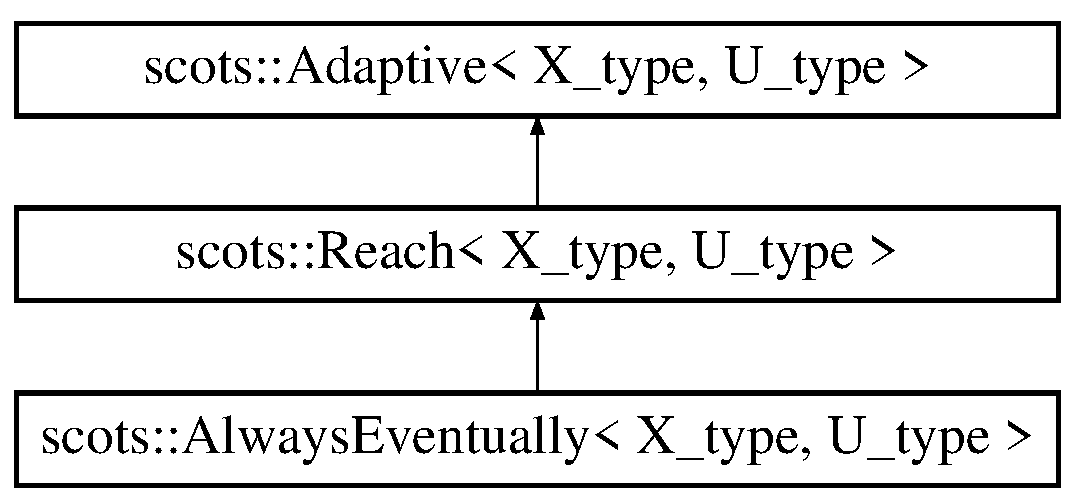
\includegraphics[height=3.000000cm]{classscots_1_1Reach}
\end{center}
\end{figure}
\subsection*{Public Member Functions}
\begin{DoxyCompactItemize}
\item 
\hyperlink{classscots_1_1Reach_a8da1e1c12f4d050f7006fafddb2c3307}{Reach} (\hyperlink{classscots_1_1System}{System} $\ast$system, double $\ast$eta\+Ratio, double tau\+Ratio, int nint, int num\+Abs, int read\+XX, int read\+Abs, char $\ast$log\+File)
\item 
\hyperlink{classscots_1_1Reach_a05425187c9015158f5495904c34342d0}{$\sim$\+Reach} ()
\item 
void \hyperlink{classscots_1_1Reach_a6787ba675345efb35d5b5dcd720cf389}{mu} (int min\+To\+Go\+Coarser, int min\+To\+Be\+Valid, int early\+Break, int verbose, int $\ast$cur\+Abs, int $\ast$iter, int $\ast$just\+Coarsed, int $\ast$iter\+Cur\+Abs, int $\ast$reached, int $\ast$stop)
\item 
int \hyperlink{classscots_1_1Reach_aae2c35919866a8235f822542a4bb3dfe}{reach} (int start\+Abs, int min\+To\+Go\+Coarser, int min\+To\+Be\+Valid, int early\+Break, int verbose=1)
\item 
{\footnotesize template$<$class G\+\_\+type , class I\+\_\+type $>$ }\\void \hyperlink{classscots_1_1Reach_ad49c77293343ad0ce4f36c9deee45f00}{initialize\+Reach} (G\+\_\+type addG, I\+\_\+type addI)
\item 
void \hyperlink{classscots_1_1Reach_ada9bf5083703b737976effb85de28c4b}{save\+CZ} (int cur\+Abs)
\item 
void \hyperlink{classscots_1_1Reach_ab9c39fa2834a0a8f08abe48838ae1c41}{save\+Verify} ()
\end{DoxyCompactItemize}
\subsection*{Public Attributes}
\begin{DoxyCompactItemize}
\item 
vector$<$ Symbolic\+Set $\ast$ $>$ \hyperlink{classscots_1_1Reach_af3fd5ddf192d97ec5dc650ad57e6c485}{Gs\+\_\+}
\item 
vector$<$ Symbolic\+Set $\ast$ $>$ \hyperlink{classscots_1_1Reach_a3366767e4a2edbb8c683e0a74a709b10}{Is\+\_\+}
\item 
vector$<$ Symbolic\+Set $\ast$ $>$ \hyperlink{classscots_1_1Reach_a2f484ac1e7bd5a451b409c373149369c}{valid\+Zs\+\_\+}
\item 
vector$<$ Symbolic\+Set $\ast$ $>$ \hyperlink{classscots_1_1Reach_ade8c2425a8ff0cc7d7ed017412b6aa29}{valid\+Cs\+\_\+}
\item 
vector$<$ Symbolic\+Set $\ast$ $>$ \hyperlink{classscots_1_1Reach_a42e41806d2c3308e41de9b21afae2206}{final\+Cs\+\_\+}
\item 
vector$<$ Symbolic\+Set $\ast$ $>$ \hyperlink{classscots_1_1Reach_ae607710b3da219ec741f8609f870bafd}{final\+Zs\+\_\+}
\end{DoxyCompactItemize}


\subsection{Detailed Description}
\subsubsection*{template$<$class X\+\_\+type, class U\+\_\+type$>$\newline
class scots\+::\+Reach$<$ X\+\_\+type, U\+\_\+type $>$}

A class (derived from base \hyperlink{classscots_1_1Adaptive}{Adaptive}) that does adaptive multiscale abstraction-\/based synthesis for a reach specification. 

\subsection{Constructor \& Destructor Documentation}
\mbox{\Hypertarget{classscots_1_1Reach_a8da1e1c12f4d050f7006fafddb2c3307}\label{classscots_1_1Reach_a8da1e1c12f4d050f7006fafddb2c3307}} 
\index{scots\+::\+Reach@{scots\+::\+Reach}!Reach@{Reach}}
\index{Reach@{Reach}!scots\+::\+Reach@{scots\+::\+Reach}}
\subsubsection{\texorpdfstring{Reach()}{Reach()}}
{\footnotesize\ttfamily template$<$class X\+\_\+type , class U\+\_\+type $>$ \\
\hyperlink{classscots_1_1Reach}{scots\+::\+Reach}$<$ X\+\_\+type, U\+\_\+type $>$\+::\hyperlink{classscots_1_1Reach}{Reach} (\begin{DoxyParamCaption}\item[{\hyperlink{classscots_1_1System}{System} $\ast$}]{system,  }\item[{double $\ast$}]{eta\+Ratio,  }\item[{double}]{tau\+Ratio,  }\item[{int}]{nint,  }\item[{int}]{num\+Abs,  }\item[{int}]{read\+XX,  }\item[{int}]{read\+Abs,  }\item[{char $\ast$}]{log\+File }\end{DoxyParamCaption})\hspace{0.3cm}{\ttfamily [inline]}}

Constructor for a \hyperlink{classscots_1_1Reach}{Reach} object. \mbox{\Hypertarget{classscots_1_1Reach_a05425187c9015158f5495904c34342d0}\label{classscots_1_1Reach_a05425187c9015158f5495904c34342d0}} 
\index{scots\+::\+Reach@{scots\+::\+Reach}!````~Reach@{$\sim$\+Reach}}
\index{````~Reach@{$\sim$\+Reach}!scots\+::\+Reach@{scots\+::\+Reach}}
\subsubsection{\texorpdfstring{$\sim$\+Reach()}{~Reach()}}
{\footnotesize\ttfamily template$<$class X\+\_\+type , class U\+\_\+type $>$ \\
\hyperlink{classscots_1_1Reach}{scots\+::\+Reach}$<$ X\+\_\+type, U\+\_\+type $>$\+::$\sim$\hyperlink{classscots_1_1Reach}{Reach} (\begin{DoxyParamCaption}{ }\end{DoxyParamCaption})\hspace{0.3cm}{\ttfamily [inline]}}

Deconstructor for a \hyperlink{classscots_1_1Reach}{Reach} object. 

\subsection{Member Function Documentation}
\mbox{\Hypertarget{classscots_1_1Reach_ad49c77293343ad0ce4f36c9deee45f00}\label{classscots_1_1Reach_ad49c77293343ad0ce4f36c9deee45f00}} 
\index{scots\+::\+Reach@{scots\+::\+Reach}!initialize\+Reach@{initialize\+Reach}}
\index{initialize\+Reach@{initialize\+Reach}!scots\+::\+Reach@{scots\+::\+Reach}}
\subsubsection{\texorpdfstring{initialize\+Reach()}{initializeReach()}}
{\footnotesize\ttfamily template$<$class X\+\_\+type , class U\+\_\+type $>$ \\
template$<$class G\+\_\+type , class I\+\_\+type $>$ \\
void \hyperlink{classscots_1_1Reach}{scots\+::\+Reach}$<$ X\+\_\+type, U\+\_\+type $>$\+::initialize\+Reach (\begin{DoxyParamCaption}\item[{G\+\_\+type}]{addG,  }\item[{I\+\_\+type}]{addI }\end{DoxyParamCaption})\hspace{0.3cm}{\ttfamily [inline]}}

Initializes objects specific to the following specifications\+: always-\/eventually, reach-\/while-\/avoid. 
\begin{DoxyParams}[1]{Parameters}
\mbox{\tt in}  & {\em addG} & Function pointer specifying the points that should be added to the goal set. \\
\hline
\mbox{\tt in}  & {\em addI} & Function pointer specifying the points that should be added to the initial set. \\
\hline
\end{DoxyParams}
\mbox{\Hypertarget{classscots_1_1Reach_a6787ba675345efb35d5b5dcd720cf389}\label{classscots_1_1Reach_a6787ba675345efb35d5b5dcd720cf389}} 
\index{scots\+::\+Reach@{scots\+::\+Reach}!mu@{mu}}
\index{mu@{mu}!scots\+::\+Reach@{scots\+::\+Reach}}
\subsubsection{\texorpdfstring{mu()}{mu()}}
{\footnotesize\ttfamily template$<$class X\+\_\+type , class U\+\_\+type $>$ \\
void \hyperlink{classscots_1_1Reach}{scots\+::\+Reach}$<$ X\+\_\+type, U\+\_\+type $>$\+::mu (\begin{DoxyParamCaption}\item[{int}]{min\+To\+Go\+Coarser,  }\item[{int}]{min\+To\+Be\+Valid,  }\item[{int}]{early\+Break,  }\item[{int}]{verbose,  }\item[{int $\ast$}]{cur\+Abs,  }\item[{int $\ast$}]{iter,  }\item[{int $\ast$}]{just\+Coarsed,  }\item[{int $\ast$}]{iter\+Cur\+Abs,  }\item[{int $\ast$}]{reached,  }\item[{int $\ast$}]{stop }\end{DoxyParamCaption})\hspace{0.3cm}{\ttfamily [inline]}}

One iteration in an adaptive minimal fixed point. 
\begin{DoxyParams}[1]{Parameters}
\mbox{\tt in}  & {\em min\+To\+Go\+Coarser} & Minimum number of iterations at an abstraction (not coarsest) before attemping to project to the next coarser abstraction. \\
\hline
\mbox{\tt in}  & {\em min\+To\+Be\+Valid} & Minimum number of iterations at an abstraction (not finest) after having gone coarser before a controller is declared valid and saved as a backup. \\
\hline
\mbox{\tt in}  & {\em early\+Break} & Whether the fixed point should end as soon as a strategy exists for the initial state. \\
\hline
\mbox{\tt in}  & {\em verbose} & Whether messages detailing the steps of the algorithm should be printed to the log file. \\
\hline
\mbox{\tt in,out}  & {\em cur\+Abs} & 0-\/index of the abstraction under consideration for the current iteration. \\
\hline
\mbox{\tt in,out}  & {\em iter} & Counter for the total number of iterations of the minimal fixed point. \\
\hline
\mbox{\tt in,out}  & {\em just\+Coarsed} & Status of the abstraction under consideration. \\
\hline
\mbox{\tt in,out}  & {\em iter\+Cur\+Abs} & Counter for the consecutive number of iterations for the current abstraction. \\
\hline
\mbox{\tt in,out}  & {\em reached} & Whether the initial state has been declared winning. \\
\hline
\mbox{\tt in,out}  & {\em stop} & Whether the fixed point should end. \\
\hline
\end{DoxyParams}
\mbox{\Hypertarget{classscots_1_1Reach_aae2c35919866a8235f822542a4bb3dfe}\label{classscots_1_1Reach_aae2c35919866a8235f822542a4bb3dfe}} 
\index{scots\+::\+Reach@{scots\+::\+Reach}!reach@{reach}}
\index{reach@{reach}!scots\+::\+Reach@{scots\+::\+Reach}}
\subsubsection{\texorpdfstring{reach()}{reach()}}
{\footnotesize\ttfamily template$<$class X\+\_\+type , class U\+\_\+type $>$ \\
int \hyperlink{classscots_1_1Reach}{scots\+::\+Reach}$<$ X\+\_\+type, U\+\_\+type $>$\+::reach (\begin{DoxyParamCaption}\item[{int}]{start\+Abs,  }\item[{int}]{min\+To\+Go\+Coarser,  }\item[{int}]{min\+To\+Be\+Valid,  }\item[{int}]{early\+Break,  }\item[{int}]{verbose = {\ttfamily 1} }\end{DoxyParamCaption})\hspace{0.3cm}{\ttfamily [inline]}}

Writes, should they exist, a sequence of controller and controller domain B\+D\+Ds to directories \textquotesingle{}C\textquotesingle{} and \textquotesingle{}Z\textquotesingle{} respectively that satisfy the reachability specification. 
\begin{DoxyParams}[1]{Parameters}
\mbox{\tt in}  & {\em start\+Abs} & 0-\/index of the abstraction to start with. \\
\hline
\mbox{\tt in}  & {\em min\+To\+Go\+Coarser} & Minimum number of growing fixed point iterations needed before an attempt to go to a coarser abstraction. \\
\hline
\mbox{\tt in}  & {\em min\+To\+Be\+Valid} & Minimum number of growing fixed point iterations needed before a controller is declared valid. \\
\hline
\mbox{\tt in}  & {\em early\+Break} & If 1, the synthesis ends as soon as I meets the domain of C. \\
\hline
\mbox{\tt in}  & {\em verbose} & If 1, prints additional information during synthesis to the log file.\\
\hline
\end{DoxyParams}
\begin{DoxyReturn}{Returns}
1 if controller(s) satisfying specification is/are synthesized; 0 otherwise. 
\end{DoxyReturn}
\mbox{\Hypertarget{classscots_1_1Reach_ada9bf5083703b737976effb85de28c4b}\label{classscots_1_1Reach_ada9bf5083703b737976effb85de28c4b}} 
\index{scots\+::\+Reach@{scots\+::\+Reach}!save\+CZ@{save\+CZ}}
\index{save\+CZ@{save\+CZ}!scots\+::\+Reach@{scots\+::\+Reach}}
\subsubsection{\texorpdfstring{save\+C\+Z()}{saveCZ()}}
{\footnotesize\ttfamily template$<$class X\+\_\+type , class U\+\_\+type $>$ \\
void \hyperlink{classscots_1_1Reach}{scots\+::\+Reach}$<$ X\+\_\+type, U\+\_\+type $>$\+::save\+CZ (\begin{DoxyParamCaption}\item[{int}]{cur\+Abs }\end{DoxyParamCaption})\hspace{0.3cm}{\ttfamily [inline]}}

Saves a snapshot of a controller and its domain into the sequence of final controllers and controller domains. 
\begin{DoxyParams}[1]{Parameters}
\mbox{\tt in}  & {\em cur\+Abs} & 0-\/index of the abstraction which the controller and controller domain that should be saved belong to. \\
\hline
\end{DoxyParams}
\mbox{\Hypertarget{classscots_1_1Reach_ab9c39fa2834a0a8f08abe48838ae1c41}\label{classscots_1_1Reach_ab9c39fa2834a0a8f08abe48838ae1c41}} 
\index{scots\+::\+Reach@{scots\+::\+Reach}!save\+Verify@{save\+Verify}}
\index{save\+Verify@{save\+Verify}!scots\+::\+Reach@{scots\+::\+Reach}}
\subsubsection{\texorpdfstring{save\+Verify()}{saveVerify()}}
{\footnotesize\ttfamily template$<$class X\+\_\+type , class U\+\_\+type $>$ \\
void \hyperlink{classscots_1_1Reach}{scots\+::\+Reach}$<$ X\+\_\+type, U\+\_\+type $>$\+::save\+Verify (\begin{DoxyParamCaption}{ }\end{DoxyParamCaption})\hspace{0.3cm}{\ttfamily [inline]}}

Saves and prints to log file some information related to the reachability/always-\/eventually specification. 

\subsection{Member Data Documentation}
\mbox{\Hypertarget{classscots_1_1Reach_a42e41806d2c3308e41de9b21afae2206}\label{classscots_1_1Reach_a42e41806d2c3308e41de9b21afae2206}} 
\index{scots\+::\+Reach@{scots\+::\+Reach}!final\+Cs\+\_\+@{final\+Cs\+\_\+}}
\index{final\+Cs\+\_\+@{final\+Cs\+\_\+}!scots\+::\+Reach@{scots\+::\+Reach}}
\subsubsection{\texorpdfstring{final\+Cs\+\_\+}{finalCs\_}}
{\footnotesize\ttfamily template$<$class X\+\_\+type , class U\+\_\+type $>$ \\
vector$<$Symbolic\+Set$\ast$$>$ \hyperlink{classscots_1_1Reach}{scots\+::\+Reach}$<$ X\+\_\+type, U\+\_\+type $>$\+::final\+Cs\+\_\+}

Sequence of controllers that satisfy the specification. \mbox{\Hypertarget{classscots_1_1Reach_ae607710b3da219ec741f8609f870bafd}\label{classscots_1_1Reach_ae607710b3da219ec741f8609f870bafd}} 
\index{scots\+::\+Reach@{scots\+::\+Reach}!final\+Zs\+\_\+@{final\+Zs\+\_\+}}
\index{final\+Zs\+\_\+@{final\+Zs\+\_\+}!scots\+::\+Reach@{scots\+::\+Reach}}
\subsubsection{\texorpdfstring{final\+Zs\+\_\+}{finalZs\_}}
{\footnotesize\ttfamily template$<$class X\+\_\+type , class U\+\_\+type $>$ \\
vector$<$Symbolic\+Set$\ast$$>$ \hyperlink{classscots_1_1Reach}{scots\+::\+Reach}$<$ X\+\_\+type, U\+\_\+type $>$\+::final\+Zs\+\_\+}

Sequence of domains of final\+Cs\+\_\+. \mbox{\Hypertarget{classscots_1_1Reach_af3fd5ddf192d97ec5dc650ad57e6c485}\label{classscots_1_1Reach_af3fd5ddf192d97ec5dc650ad57e6c485}} 
\index{scots\+::\+Reach@{scots\+::\+Reach}!Gs\+\_\+@{Gs\+\_\+}}
\index{Gs\+\_\+@{Gs\+\_\+}!scots\+::\+Reach@{scots\+::\+Reach}}
\subsubsection{\texorpdfstring{Gs\+\_\+}{Gs\_}}
{\footnotesize\ttfamily template$<$class X\+\_\+type , class U\+\_\+type $>$ \\
vector$<$Symbolic\+Set$\ast$$>$ \hyperlink{classscots_1_1Reach}{scots\+::\+Reach}$<$ X\+\_\+type, U\+\_\+type $>$\+::Gs\+\_\+}

Instance of $\ast$\+Xs\+\_\+\mbox{[}i\mbox{]} containing goal states. \mbox{\Hypertarget{classscots_1_1Reach_a3366767e4a2edbb8c683e0a74a709b10}\label{classscots_1_1Reach_a3366767e4a2edbb8c683e0a74a709b10}} 
\index{scots\+::\+Reach@{scots\+::\+Reach}!Is\+\_\+@{Is\+\_\+}}
\index{Is\+\_\+@{Is\+\_\+}!scots\+::\+Reach@{scots\+::\+Reach}}
\subsubsection{\texorpdfstring{Is\+\_\+}{Is\_}}
{\footnotesize\ttfamily template$<$class X\+\_\+type , class U\+\_\+type $>$ \\
vector$<$Symbolic\+Set$\ast$$>$ \hyperlink{classscots_1_1Reach}{scots\+::\+Reach}$<$ X\+\_\+type, U\+\_\+type $>$\+::Is\+\_\+}

Instance of $\ast$\+Xs\+\_\+\mbox{[}i\mbox{]} containing initial states. \mbox{\Hypertarget{classscots_1_1Reach_ade8c2425a8ff0cc7d7ed017412b6aa29}\label{classscots_1_1Reach_ade8c2425a8ff0cc7d7ed017412b6aa29}} 
\index{scots\+::\+Reach@{scots\+::\+Reach}!valid\+Cs\+\_\+@{valid\+Cs\+\_\+}}
\index{valid\+Cs\+\_\+@{valid\+Cs\+\_\+}!scots\+::\+Reach@{scots\+::\+Reach}}
\subsubsection{\texorpdfstring{valid\+Cs\+\_\+}{validCs\_}}
{\footnotesize\ttfamily template$<$class X\+\_\+type , class U\+\_\+type $>$ \\
vector$<$Symbolic\+Set$\ast$$>$ \hyperlink{classscots_1_1Reach}{scots\+::\+Reach}$<$ X\+\_\+type, U\+\_\+type $>$\+::valid\+Cs\+\_\+}

Controllers that act as savepoints. \mbox{\Hypertarget{classscots_1_1Reach_a2f484ac1e7bd5a451b409c373149369c}\label{classscots_1_1Reach_a2f484ac1e7bd5a451b409c373149369c}} 
\index{scots\+::\+Reach@{scots\+::\+Reach}!valid\+Zs\+\_\+@{valid\+Zs\+\_\+}}
\index{valid\+Zs\+\_\+@{valid\+Zs\+\_\+}!scots\+::\+Reach@{scots\+::\+Reach}}
\subsubsection{\texorpdfstring{valid\+Zs\+\_\+}{validZs\_}}
{\footnotesize\ttfamily template$<$class X\+\_\+type , class U\+\_\+type $>$ \\
vector$<$Symbolic\+Set$\ast$$>$ \hyperlink{classscots_1_1Reach}{scots\+::\+Reach}$<$ X\+\_\+type, U\+\_\+type $>$\+::valid\+Zs\+\_\+}

Contains winning states that act as savepoints. 

The documentation for this class was generated from the following file\+:\begin{DoxyCompactItemize}
\item 
/home/kylehsu/\+S\+C\+O\+T\+S-\/\+Adaptive/bdd/\hyperlink{Reach_8hh}{Reach.\+hh}\end{DoxyCompactItemize}

\hypertarget{classscots_1_1Safe}{}\section{scots\+:\+:Safe$<$ X\+\_\+type, U\+\_\+type $>$ Class Template Reference}
\label{classscots_1_1Safe}\index{scots\+::\+Safe$<$ X\+\_\+type, U\+\_\+type $>$@{scots\+::\+Safe$<$ X\+\_\+type, U\+\_\+type $>$}}


A class (derived from base \hyperlink{classscots_1_1Adaptive}{Adaptive}) that does adaptive multiscale abstraction-\/based synthesis for a safe specification.  




{\ttfamily \#include $<$Safe.\+hh$>$}

Inheritance diagram for scots\+:\+:Safe$<$ X\+\_\+type, U\+\_\+type $>$\+:\begin{figure}[H]
\begin{center}
\leavevmode
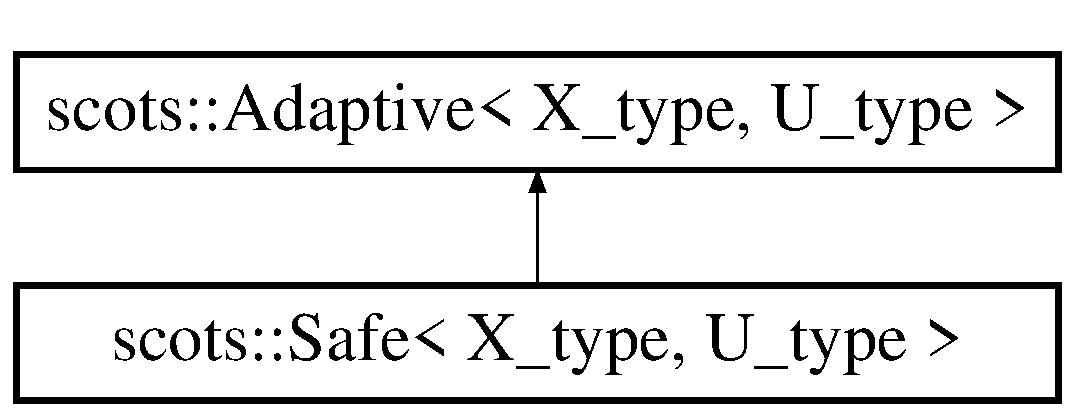
\includegraphics[height=3.000000cm]{classscots_1_1Safe}
\end{center}
\end{figure}
\subsection*{Public Member Functions}
\begin{DoxyCompactItemize}
\item 
\hyperlink{classscots_1_1Safe_ab2fd1008342b2ecccadceff25d349b6a}{Safe} (\hyperlink{classscots_1_1System}{System} $\ast$system, double $\ast$eta\+Ratio, double tau\+Ratio, int nint, int num\+Abs, int read\+XX, int read\+Abs, char $\ast$log\+File)
\item 
void \hyperlink{classscots_1_1Safe_ac9f2578f6b74602510ca5db4b2ef31b9}{nu} (int cur\+Abs)
\item 
void \hyperlink{classscots_1_1Safe_af5ea22ef6bd1f86dd1a6f7ef6e590492}{safe} ()
\item 
{\footnotesize template$<$class S\+\_\+type $>$ }\\void \hyperlink{classscots_1_1Safe_a8255c8172548f64907fedaddfcae9519}{initialize\+Safe} (S\+\_\+type addS)
\item 
void \hyperlink{classscots_1_1Safe_ab6866ae8860c91feb49467556f0a8598}{save\+Verify} ()
\end{DoxyCompactItemize}
\subsection*{Public Attributes}
\begin{DoxyCompactItemize}
\item 
vector$<$ Symbolic\+Set $\ast$ $>$ \hyperlink{classscots_1_1Safe_a4c272a1e134f26e88c74a08c2703d934}{Ss\+\_\+}
\item 
vector$<$ Symbolic\+Set $\ast$ $>$ \hyperlink{classscots_1_1Safe_a30e38b9a75a8bf34efb2512465ea9468}{inf\+Zs\+\_\+}
\end{DoxyCompactItemize}


\subsection{Detailed Description}
\subsubsection*{template$<$class X\+\_\+type, class U\+\_\+type$>$\newline
class scots\+::\+Safe$<$ X\+\_\+type, U\+\_\+type $>$}

A class (derived from base \hyperlink{classscots_1_1Adaptive}{Adaptive}) that does adaptive multiscale abstraction-\/based synthesis for a safe specification. 

\subsection{Constructor \& Destructor Documentation}
\mbox{\Hypertarget{classscots_1_1Safe_ab2fd1008342b2ecccadceff25d349b6a}\label{classscots_1_1Safe_ab2fd1008342b2ecccadceff25d349b6a}} 
\index{scots\+::\+Safe@{scots\+::\+Safe}!Safe@{Safe}}
\index{Safe@{Safe}!scots\+::\+Safe@{scots\+::\+Safe}}
\subsubsection{\texorpdfstring{Safe()}{Safe()}}
{\footnotesize\ttfamily template$<$class X\+\_\+type , class U\+\_\+type $>$ \\
\hyperlink{classscots_1_1Safe}{scots\+::\+Safe}$<$ X\+\_\+type, U\+\_\+type $>$\+::\hyperlink{classscots_1_1Safe}{Safe} (\begin{DoxyParamCaption}\item[{\hyperlink{classscots_1_1System}{System} $\ast$}]{system,  }\item[{double $\ast$}]{eta\+Ratio,  }\item[{double}]{tau\+Ratio,  }\item[{int}]{nint,  }\item[{int}]{num\+Abs,  }\item[{int}]{read\+XX,  }\item[{int}]{read\+Abs,  }\item[{char $\ast$}]{log\+File }\end{DoxyParamCaption})\hspace{0.3cm}{\ttfamily [inline]}}

Constructor for a \hyperlink{classscots_1_1Safe}{Safe} object. 

\subsection{Member Function Documentation}
\mbox{\Hypertarget{classscots_1_1Safe_a8255c8172548f64907fedaddfcae9519}\label{classscots_1_1Safe_a8255c8172548f64907fedaddfcae9519}} 
\index{scots\+::\+Safe@{scots\+::\+Safe}!initialize\+Safe@{initialize\+Safe}}
\index{initialize\+Safe@{initialize\+Safe}!scots\+::\+Safe@{scots\+::\+Safe}}
\subsubsection{\texorpdfstring{initialize\+Safe()}{initializeSafe()}}
{\footnotesize\ttfamily template$<$class X\+\_\+type , class U\+\_\+type $>$ \\
template$<$class S\+\_\+type $>$ \\
void \hyperlink{classscots_1_1Safe}{scots\+::\+Safe}$<$ X\+\_\+type, U\+\_\+type $>$\+::initialize\+Safe (\begin{DoxyParamCaption}\item[{S\+\_\+type}]{addS }\end{DoxyParamCaption})\hspace{0.3cm}{\ttfamily [inline]}}

Initializes objects specific to the following specifications\+: safe. 
\begin{DoxyParams}[1]{Parameters}
\mbox{\tt in}  & {\em addS} & Function pointer specifying the points that should be added to the potential safe set. \\
\hline
\end{DoxyParams}
\mbox{\Hypertarget{classscots_1_1Safe_ac9f2578f6b74602510ca5db4b2ef31b9}\label{classscots_1_1Safe_ac9f2578f6b74602510ca5db4b2ef31b9}} 
\index{scots\+::\+Safe@{scots\+::\+Safe}!nu@{nu}}
\index{nu@{nu}!scots\+::\+Safe@{scots\+::\+Safe}}
\subsubsection{\texorpdfstring{nu()}{nu()}}
{\footnotesize\ttfamily template$<$class X\+\_\+type , class U\+\_\+type $>$ \\
void \hyperlink{classscots_1_1Safe}{scots\+::\+Safe}$<$ X\+\_\+type, U\+\_\+type $>$\+::nu (\begin{DoxyParamCaption}\item[{int}]{cur\+Abs }\end{DoxyParamCaption})\hspace{0.3cm}{\ttfamily [inline]}}

\hyperlink{classscots_1_1Adaptive}{Adaptive} maximal fixed point. \mbox{\Hypertarget{classscots_1_1Safe_af5ea22ef6bd1f86dd1a6f7ef6e590492}\label{classscots_1_1Safe_af5ea22ef6bd1f86dd1a6f7ef6e590492}} 
\index{scots\+::\+Safe@{scots\+::\+Safe}!safe@{safe}}
\index{safe@{safe}!scots\+::\+Safe@{scots\+::\+Safe}}
\subsubsection{\texorpdfstring{safe()}{safe()}}
{\footnotesize\ttfamily template$<$class X\+\_\+type , class U\+\_\+type $>$ \\
void \hyperlink{classscots_1_1Safe}{scots\+::\+Safe}$<$ X\+\_\+type, U\+\_\+type $>$\+::safe (\begin{DoxyParamCaption}{ }\end{DoxyParamCaption})\hspace{0.3cm}{\ttfamily [inline]}}

Writes, should they exist, controllers of specified abstractions that together satisfy a safety specification. \mbox{\Hypertarget{classscots_1_1Safe_ab6866ae8860c91feb49467556f0a8598}\label{classscots_1_1Safe_ab6866ae8860c91feb49467556f0a8598}} 
\index{scots\+::\+Safe@{scots\+::\+Safe}!save\+Verify@{save\+Verify}}
\index{save\+Verify@{save\+Verify}!scots\+::\+Safe@{scots\+::\+Safe}}
\subsubsection{\texorpdfstring{save\+Verify()}{saveVerify()}}
{\footnotesize\ttfamily template$<$class X\+\_\+type , class U\+\_\+type $>$ \\
void \hyperlink{classscots_1_1Safe}{scots\+::\+Safe}$<$ X\+\_\+type, U\+\_\+type $>$\+::save\+Verify (\begin{DoxyParamCaption}{ }\end{DoxyParamCaption})\hspace{0.3cm}{\ttfamily [inline]}}

Saves and prints to log file some information related to the safety specification. 

\subsection{Member Data Documentation}
\mbox{\Hypertarget{classscots_1_1Safe_a30e38b9a75a8bf34efb2512465ea9468}\label{classscots_1_1Safe_a30e38b9a75a8bf34efb2512465ea9468}} 
\index{scots\+::\+Safe@{scots\+::\+Safe}!inf\+Zs\+\_\+@{inf\+Zs\+\_\+}}
\index{inf\+Zs\+\_\+@{inf\+Zs\+\_\+}!scots\+::\+Safe@{scots\+::\+Safe}}
\subsubsection{\texorpdfstring{inf\+Zs\+\_\+}{infZs\_}}
{\footnotesize\ttfamily template$<$class X\+\_\+type , class U\+\_\+type $>$ \\
vector$<$Symbolic\+Set$\ast$$>$ \hyperlink{classscots_1_1Safe}{scots\+::\+Safe}$<$ X\+\_\+type, U\+\_\+type $>$\+::inf\+Zs\+\_\+}

Instance of $\ast$\+Xs\+\_\+\mbox{[}i\mbox{]} containing projection of convergence of previous maximal fixed points. \mbox{\Hypertarget{classscots_1_1Safe_a4c272a1e134f26e88c74a08c2703d934}\label{classscots_1_1Safe_a4c272a1e134f26e88c74a08c2703d934}} 
\index{scots\+::\+Safe@{scots\+::\+Safe}!Ss\+\_\+@{Ss\+\_\+}}
\index{Ss\+\_\+@{Ss\+\_\+}!scots\+::\+Safe@{scots\+::\+Safe}}
\subsubsection{\texorpdfstring{Ss\+\_\+}{Ss\_}}
{\footnotesize\ttfamily template$<$class X\+\_\+type , class U\+\_\+type $>$ \\
vector$<$Symbolic\+Set$\ast$$>$ \hyperlink{classscots_1_1Safe}{scots\+::\+Safe}$<$ X\+\_\+type, U\+\_\+type $>$\+::Ss\+\_\+}

Instance of $\ast$\+Xs\+\_\+\mbox{[}i\mbox{]} containing safe states. 

The documentation for this class was generated from the following file\+:\begin{DoxyCompactItemize}
\item 
/home/kylehsu/\+S\+C\+O\+T\+S-\/\+Adaptive/bdd/Safe.\+hh\end{DoxyCompactItemize}

\chapter{File Documentation}
\hypertarget{Adaptive_8hh}{}\section{/home/kylehsu/\+S\+C\+O\+T\+S-\/\+Adaptive/bdd/\+Adaptive.hh File Reference}
\label{Adaptive_8hh}\index{/home/kylehsu/\+S\+C\+O\+T\+S-\/\+Adaptive/bdd/\+Adaptive.\+hh@{/home/kylehsu/\+S\+C\+O\+T\+S-\/\+Adaptive/bdd/\+Adaptive.\+hh}}
{\ttfamily \#include $<$cstdio$>$}\newline
{\ttfamily \#include $<$vector$>$}\newline
{\ttfamily \#include \char`\"{}Symbolic\+Model\+Growth\+Bound.\+hh\char`\"{}}\newline
{\ttfamily \#include \char`\"{}Fixed\+Point.\+hh\char`\"{}}\newline
{\ttfamily \#include \char`\"{}Profile.\+hh\char`\"{}}\newline
{\ttfamily \#include \char`\"{}Helper.\+hh\char`\"{}}\newline
\subsection*{Classes}
\begin{DoxyCompactItemize}
\item 
class \hyperlink{classscots_1_1Adaptive}{scots\+::\+Adaptive$<$ X\+\_\+type, U\+\_\+type $>$}
\begin{DoxyCompactList}\small\item\em A class that does abstraction-\/based synthesis with adaptive time-\/ and state space-\/gridding. \end{DoxyCompactList}\end{DoxyCompactItemize}


\subsection{Detailed Description}
Contains the Adaptive class. 
\hypertarget{AlwaysEventually_8hh}{}\section{/home/kylehsu/\+S\+C\+O\+T\+S-\/\+Adaptive/bdd/\+Always\+Eventually.hh File Reference}
\label{AlwaysEventually_8hh}\index{/home/kylehsu/\+S\+C\+O\+T\+S-\/\+Adaptive/bdd/\+Always\+Eventually.\+hh@{/home/kylehsu/\+S\+C\+O\+T\+S-\/\+Adaptive/bdd/\+Always\+Eventually.\+hh}}
{\ttfamily \#include \char`\"{}Reach.\+hh\char`\"{}}\newline
\subsection*{Classes}
\begin{DoxyCompactItemize}
\item 
class \hyperlink{classscots_1_1AlwaysEventually}{scots\+::\+Always\+Eventually$<$ X\+\_\+type, U\+\_\+type $>$}
\begin{DoxyCompactList}\small\item\em A class (derived from base \hyperlink{classscots_1_1Adaptive}{Adaptive}) that does adaptive multiscale abstraction-\/based synthesis for an always-\/eventually specification. \end{DoxyCompactList}\end{DoxyCompactItemize}


\subsection{Detailed Description}
Contains the Always\+Eventually class. 
\hypertarget{Compare_8hh}{}\section{/home/kylehsu/\+S\+C\+O\+T\+S-\/\+Adaptive/bdd/\+Compare.hh File Reference}
\label{Compare_8hh}\index{/home/kylehsu/\+S\+C\+O\+T\+S-\/\+Adaptive/bdd/\+Compare.\+hh@{/home/kylehsu/\+S\+C\+O\+T\+S-\/\+Adaptive/bdd/\+Compare.\+hh}}
{\ttfamily \#include $<$cstdio$>$}\newline
{\ttfamily \#include $<$vector$>$}\newline
{\ttfamily \#include \char`\"{}Symbolic\+Model\+Growth\+Bound.\+hh\char`\"{}}\newline
{\ttfamily \#include \char`\"{}Fixed\+Point.\+hh\char`\"{}}\newline
{\ttfamily \#include \char`\"{}Runge\+Kutta4.\+hh\char`\"{}}\newline
{\ttfamily \#include \char`\"{}Profile.\+hh\char`\"{}}\newline
{\ttfamily \#include \char`\"{}Tic\+Toc.\+hh\char`\"{}}\newline
{\ttfamily \#include \char`\"{}Helper.\+hh\char`\"{}}\newline
\subsection*{Classes}
\begin{DoxyCompactItemize}
\item 
class \hyperlink{classscots_1_1Compare}{scots\+::\+Compare$<$ X\+\_\+type, U\+\_\+type $>$}
\begin{DoxyCompactList}\small\item\em A class that provides comparison using basic S\+C\+O\+TS. \end{DoxyCompactList}\end{DoxyCompactItemize}


\subsection{Detailed Description}
Contains the Compare class. 
\hypertarget{Reach_8hh}{}\section{/home/kylehsu/\+S\+C\+O\+T\+S-\/\+Adaptive/bdd/\+Reach.hh File Reference}
\label{Reach_8hh}\index{/home/kylehsu/\+S\+C\+O\+T\+S-\/\+Adaptive/bdd/\+Reach.\+hh@{/home/kylehsu/\+S\+C\+O\+T\+S-\/\+Adaptive/bdd/\+Reach.\+hh}}
{\ttfamily \#include \char`\"{}Adaptive.\+hh\char`\"{}}\newline
\subsection*{Classes}
\begin{DoxyCompactItemize}
\item 
class \hyperlink{classscots_1_1Reach}{scots\+::\+Reach$<$ X\+\_\+type, U\+\_\+type $>$}
\begin{DoxyCompactList}\small\item\em A class (derived from base \hyperlink{classscots_1_1Adaptive}{Adaptive}) that does adaptive multiscale abstraction-\/based synthesis for a reach specification. \end{DoxyCompactList}\end{DoxyCompactItemize}


\subsection{Detailed Description}
Contains the Reach class.

Contains the Safe class. 
\hypertarget{Helper_8hh}{}\section{/home/kylehsu/\+S\+C\+O\+T\+S-\/\+Adaptive/utils/\+Helper.hh File Reference}
\label{Helper_8hh}\index{/home/kylehsu/\+S\+C\+O\+T\+S-\/\+Adaptive/utils/\+Helper.\+hh@{/home/kylehsu/\+S\+C\+O\+T\+S-\/\+Adaptive/utils/\+Helper.\+hh}}
{\ttfamily \#include $<$dirent.\+h$>$}\newline
{\ttfamily \#include $<$sys/stat.\+h$>$}\newline
{\ttfamily \#include $<$sys/types.\+h$>$}\newline
{\ttfamily \#include $<$string$>$}\newline
{\ttfamily \#include \char`\"{}Symbolic\+Set.\+hh\char`\"{}}\newline
\subsection*{Functions}
\begin{DoxyCompactItemize}
\item 
{\footnotesize template$<$class dir\+\_\+type $>$ }\\void \hyperlink{Helper_8hh_a54c684ce784017d4c61e9fc7a179be67}{helper\+::check\+Make\+Dir} (dir\+\_\+type dir\+Name)
\item 
{\footnotesize template$<$class array\+\_\+type $>$ }\\void \hyperlink{Helper_8hh_ad3a9b9a5d8b46962dae72719f691201c}{helper\+::print\+Array} (array\+\_\+type array, int size)
\item 
{\footnotesize template$<$class vec\+\_\+type , class prefix\+\_\+type $>$ }\\void \hyperlink{Helper_8hh_afea778bfb31cba93e003c382413c36b2}{helper\+::save\+Vec} (vec\+\_\+type vec, prefix\+\_\+type vec\+Prefix)
\item 
{\footnotesize template$<$class vec\+\_\+type $>$ }\\void \hyperlink{Helper_8hh_a4cfbf4be07fc1d320df3c06ab77ff469}{helper\+::delete\+Vec} (vec\+\_\+type vec)
\item 
{\footnotesize template$<$class vec\+\_\+type , class prefix\+\_\+type $>$ }\\void \hyperlink{Helper_8hh_a33cb7ae024bddfc7874b8aaa80d46f4b}{helper\+::print\+Vec} (vec\+\_\+type vec, prefix\+\_\+type vec\+Prefix)
\item 
{\footnotesize template$<$class vec\+\_\+type $>$ }\\void \hyperlink{Helper_8hh_a204cd701ae182be7b10e2017e259285b}{helper\+::delete\+Vec\+Array} (vec\+\_\+type vec)
\end{DoxyCompactItemize}


\subsection{Detailed Description}
Contains helper functions. 

\subsection{Function Documentation}
\mbox{\Hypertarget{Helper_8hh_file_a54c684ce784017d4c61e9fc7a179be67}\label{Helper_8hh_file_a54c684ce784017d4c61e9fc7a179be67}} 
\index{Helper.\+hh@{Helper.\+hh}!check\+Make\+Dir@{check\+Make\+Dir}}
\index{check\+Make\+Dir@{check\+Make\+Dir}!Helper.\+hh@{Helper.\+hh}}
\subsubsection{\texorpdfstring{check\+Make\+Dir()}{checkMakeDir()}}
{\footnotesize\ttfamily template$<$class dir\+\_\+type $>$ \\
void helper\+::check\+Make\+Dir (\begin{DoxyParamCaption}\item[{dir\+\_\+type}]{dir\+Name }\end{DoxyParamCaption})}

Ensures that a specified subdirectory exists. 
\begin{DoxyParams}[1]{Parameters}
\mbox{\tt in}  & {\em dir\+Name} & Name of the desired subdirectory. \\
\hline
\end{DoxyParams}
\mbox{\Hypertarget{Helper_8hh_file_a4cfbf4be07fc1d320df3c06ab77ff469}\label{Helper_8hh_file_a4cfbf4be07fc1d320df3c06ab77ff469}} 
\index{Helper.\+hh@{Helper.\+hh}!delete\+Vec@{delete\+Vec}}
\index{delete\+Vec@{delete\+Vec}!Helper.\+hh@{Helper.\+hh}}
\subsubsection{\texorpdfstring{delete\+Vec()}{deleteVec()}}
{\footnotesize\ttfamily template$<$class vec\+\_\+type $>$ \\
void helper\+::delete\+Vec (\begin{DoxyParamCaption}\item[{vec\+\_\+type}]{vec }\end{DoxyParamCaption})}

Frees a vector\textquotesingle{}s objects from heap memory. 
\begin{DoxyParams}[1]{Parameters}
\mbox{\tt in}  & {\em vec} & Vector of objects. \\
\hline
\end{DoxyParams}
\mbox{\Hypertarget{Helper_8hh_file_a204cd701ae182be7b10e2017e259285b}\label{Helper_8hh_file_a204cd701ae182be7b10e2017e259285b}} 
\index{Helper.\+hh@{Helper.\+hh}!delete\+Vec\+Array@{delete\+Vec\+Array}}
\index{delete\+Vec\+Array@{delete\+Vec\+Array}!Helper.\+hh@{Helper.\+hh}}
\subsubsection{\texorpdfstring{delete\+Vec\+Array()}{deleteVecArray()}}
{\footnotesize\ttfamily template$<$class vec\+\_\+type $>$ \\
void helper\+::delete\+Vec\+Array (\begin{DoxyParamCaption}\item[{vec\+\_\+type}]{vec }\end{DoxyParamCaption})}

Frees a vector\textquotesingle{}s arrays from heap memory. 
\begin{DoxyParams}[1]{Parameters}
\mbox{\tt in}  & {\em vec} & Vector of arrays. \\
\hline
\end{DoxyParams}
\mbox{\Hypertarget{Helper_8hh_file_ad3a9b9a5d8b46962dae72719f691201c}\label{Helper_8hh_file_ad3a9b9a5d8b46962dae72719f691201c}} 
\index{Helper.\+hh@{Helper.\+hh}!print\+Array@{print\+Array}}
\index{print\+Array@{print\+Array}!Helper.\+hh@{Helper.\+hh}}
\subsubsection{\texorpdfstring{print\+Array()}{printArray()}}
{\footnotesize\ttfamily template$<$class array\+\_\+type $>$ \\
void helper\+::print\+Array (\begin{DoxyParamCaption}\item[{array\+\_\+type}]{array,  }\item[{int}]{size }\end{DoxyParamCaption})}

Prints the contents of an array to a log file. 
\begin{DoxyParams}[1]{Parameters}
\mbox{\tt in}  & {\em array} & Array. \\
\hline
\mbox{\tt in}  & {\em size} & Number of elements. \\
\hline
\end{DoxyParams}
\mbox{\Hypertarget{Helper_8hh_file_a33cb7ae024bddfc7874b8aaa80d46f4b}\label{Helper_8hh_file_a33cb7ae024bddfc7874b8aaa80d46f4b}} 
\index{Helper.\+hh@{Helper.\+hh}!print\+Vec@{print\+Vec}}
\index{print\+Vec@{print\+Vec}!Helper.\+hh@{Helper.\+hh}}
\subsubsection{\texorpdfstring{print\+Vec()}{printVec()}}
{\footnotesize\ttfamily template$<$class vec\+\_\+type , class prefix\+\_\+type $>$ \\
void helper\+::print\+Vec (\begin{DoxyParamCaption}\item[{vec\+\_\+type}]{vec,  }\item[{prefix\+\_\+type}]{vec\+Prefix }\end{DoxyParamCaption})}

Prints a vector\textquotesingle{}s Symbolic\+Sets to the console. 
\begin{DoxyParams}[1]{Parameters}
\mbox{\tt in}  & {\em vec} & Vector of Symbolic\+Sets. \\
\hline
\mbox{\tt in}  & {\em vec\+Prefix} & Name of a Symbolic\+Set. \\
\hline
\end{DoxyParams}
\mbox{\Hypertarget{Helper_8hh_file_afea778bfb31cba93e003c382413c36b2}\label{Helper_8hh_file_afea778bfb31cba93e003c382413c36b2}} 
\index{Helper.\+hh@{Helper.\+hh}!save\+Vec@{save\+Vec}}
\index{save\+Vec@{save\+Vec}!Helper.\+hh@{Helper.\+hh}}
\subsubsection{\texorpdfstring{save\+Vec()}{saveVec()}}
{\footnotesize\ttfamily template$<$class vec\+\_\+type , class prefix\+\_\+type $>$ \\
void helper\+::save\+Vec (\begin{DoxyParamCaption}\item[{vec\+\_\+type}]{vec,  }\item[{prefix\+\_\+type}]{vec\+Prefix }\end{DoxyParamCaption})}

Writes a vector of Symbolic\+Sets into a subdirectory. 
\begin{DoxyParams}[1]{Parameters}
\mbox{\tt in}  & {\em vec} & Vector of Symbolic\+Sets. \\
\hline
\mbox{\tt in}  & {\em vec\+Prefix} & Subdirectory name + \textquotesingle{}/\textquotesingle{} + filename prefix. \\
\hline
\end{DoxyParams}

%--- End generated contents ---

% Index
\backmatter
\newpage
\phantomsection
\clearemptydoublepage
\addcontentsline{toc}{chapter}{Index}
\printindex

\end{document}
